%%%%%%%%%%%%%%%%%%%%%%
%usenix
%\documentclass[letterpaper,twocolumn,10pt]{article}
%\usepackage{usenix2019,epsfig,endnotes}
%%%%%%%%%%%%%%%%%%%%%%
%CCS
%\documentclass[sigconf, anonymous]{acmart}

% remove reference format for submission
%\settopmatter{printacmref=false}

% remove copyright box for submission
%\renewcommand\footnotetextcopyrightpermission[1]{}

% control headers 
%\fancyhf{} 
%\fancyhead[C]{Anonymous submission \#9999 to ACM CCS 2019} % TODO: replace 9999 with your paper number
%\fancyfoot[C]{\thepage}

%\setcopyright{none} % No copyright notice required for submissions
%\acmConference[Anonymous Submission to ACM CCS 2019]{ACM Conference on Computer and Communications Security}{Due 5 February 2019}{London, UK}
%\acmYear{2019}

%%%%%%%%%%%%%%%%%%%%%%

%S&P
\documentclass[conference]{IEEEtran}

\newif\ifdraft
%\drafttrue

\usepackage{xcolor}
\usepackage{graphicx,pifont}
\usepackage{adjustbox}
\usepackage{caption}
\usepackage{subcaption}
\usepackage{mathtools}
\usepackage{mathrsfs}
\usepackage{xspace}
\usepackage{url}
\usepackage{pifont}
\usepackage{listings}
\usepackage{multirow, bigdelim}
\usepackage{wasysym}
\usepackage{array}
\usepackage[mode=buildnew]{standalone}
\usepackage{rotating}
\usepackage{graphicx}
\usepackage{tikz}
\usetikzlibrary{positioning}
\usetikzlibrary{shapes,arrows}

%\usepackage[font={small}]{caption}
%\usepackage{enumitem}
\usepackage{cite}
%\usepackage{flushend}
\usepackage{hyperref}
%\usepackage{caption}



%% Compacting 
%%
%\usepackage[
%all=normal,floats=tight
%,paragraphs=tight
%,wordspacing=tight
%,mathspacing=tight
%,mathdisplays=tight
%]{savetrees}
%\usepackage[compact]{titlesec}


\lstset{
  basicstyle=\ttfamily,
  numbers=left, xleftmargin=2em,frame=single,framexleftmargin=1.5em,
  %numberstyle=\tiny,
  columns=fullflexible,
  showstringspaces=false,
  commentstyle=\color{gray}\upshape
}

\lstdefinelanguage{HTML}
{
  morestring=[b]",
  morestring=[s]{>}{<},
  morecomment=[s]{<?}{?>},
  stringstyle=\color{black},
  identifierstyle=\color{darkblue},
  keywordstyle=\color{blue},
  morekeywords={form,input,encrypted,Input}
}

\colorlet{punct}{red!70!black}
\definecolor{background}{HTML}{EEEEEE}
\definecolor{delim}{RGB}{20,105,176}
\colorlet{numb}{magenta!20!black}

\lstdefinelanguage{json}{
    basicstyle=\small\ttfamily,
    numbers=left,
    numberstyle=\scriptsize,
    stepnumber=1,
    numbersep=8pt,
    showstringspaces=false,
    breaklines=true,
    frame=lines,
    backgroundcolor=\color{background},
    morekeywords={formId, formName, signature, ui, dim, id, type, label, text, trigger, domain, sizeH, sizeW, size_x, size_y, enable, uiGap, size},
    literate=
     *{0}{{{\color{numb}0}}}{1}
      {1}{{{\color{numb}1}}}{1}
      {2}{{{\color{numb}2}}}{1}
      {3}{{{\color{numb}3}}}{1}
      {4}{{{\color{numb}4}}}{1}
      {5}{{{\color{numb}5}}}{1}
      {6}{{{\color{numb}6}}}{1}
      {7}{{{\color{numb}7}}}{1}
      {8}{{{\color{numb}8}}}{1}
      {9}{{{\color{numb}9}}}{1}
      {:}{{{\color{punct}{:}}}}{1}
      {,}{{{\color{punct}{,}}}}{1}
      {\{}{{{\color{delim}{\{}}}}{1}
      {\}}{{{\color{delim}{\}}}}}{1}
      {[}{{{\color{delim}{[}}}}{1}
      {]}{{{\color{delim}{]}}}}{1},
}

\renewcommand\lstlistingname{Specification}

\let\oldding\ding% Store old \ding in \oldding
\renewcommand{\ding}[2][1]{\scalebox{#1}{\oldding{#2}}}% Scale \oldding via optional argument

\newcommand{\zero}{\ding[1.2]{171}\xspace}
\newcommand{\one}{\ding[1.2]{172}\xspace}
\newcommand{\two}{\ding[1.2]{173}\xspace}
\newcommand{\three}{\ding[1.2]{174}\xspace}
\newcommand{\four}{\ding[1.2]{175}\xspace}
\newcommand{\five}{\ding[1.2]{176}\xspace}
\newcommand{\six}{\ding[1.2]{177}\xspace}
\newcommand{\seven}{\ding[1.2]{178}\xspace}
\newcommand{\eight}{\ding[1.2]{179}\xspace}
\newcommand{\nine}{\ding[1.2]{180}\xspace}
\newcommand{\ten}{\ding[1.2]{181}\xspace}

\usepackage{color, colortbl}
\definecolor{gray}{rgb}{0.4,0.4,0.4}
\definecolor{darkblue}{rgb}{0.0,0.0,0.6}
\definecolor{cyan}{rgb}{0.0,0.6,0.6}
%\definecolor{Gray}{gray}{0.1}

\definecolor{Gray}{rgb}{0.88, 0.88, 0.88}
\definecolor{HGray}{rgb}{0.7, 0.7, 0.7}
%\definecolor{HGray}{gray}{0.8}

\newcommand{\yes}{\CIRCLE} 
\newcommand{\no}{\Circle} 
\newcommand{\yesNope}{\LEFTcircle} 


\newcommand{\red}[1]{\textcolor{red}{#1}} 

\newcommand{\ad}[1]{\textcolor{red}{Aritra: #1}}
\newcommand{\srdjan}[1]{\textcolor{brown}{Srdjan: #1}}
\newcommand{\todo}[1]{\textcolor{red}{TODO: #1}}
\newcommand{\tocite}{\textcolor{blue}{[cite]}}

%\widowpenalty 200000
%\clubpenalty 200000
%\usepackage[compact]{titlesec}

\newcommand{\name}{\textsc{GuardIOn}\xspace}
\newcommand{\tool}{\name}
\newcommand{\device}{\textsc{Bridge}\xspace}
\newcommand{\pop}{proof-of-pointer\xspace}
\newcommand{\Pop}{Proof-of-pointer\xspace}

\newcommand{\poa}{proof-of-action\xspace}
\newcommand{\Poa}{Proof-of-action\xspace}

\newcommand{\poui}{proof-of-UI\xspace}
\newcommand{\Poui}{Proof-of-UI\xspace}
\newcommand{\server}{\textsc{Server}\xspace}

\newcommand{\toolname}{\name\xspace}

\newcommand{\usb}{USB\xspace}
\newcommand{\bluetooth}{Bluetooth\xspace}
\newcommand{\webusb}{WebUSB\xspace}
\newcommand{\html}{HTML\xspace}
\newcommand{\webbt}{WebBluetooth\xspace}
\newcommand{\http}{HTTP\xspace}
\newcommand{\https}{HTTPS\xspace}
\newcommand{\tls}{TLS\xspace}
\newcommand{\ssl}{\texttt{SSl}\xspace}
\newcommand{\onSelect}{\texttt{onSelect()}\xspace}

%\newcommand{\myparagraph}[1]{{\scshape \bfseries #1.}}
\newcommand{\myparagraph}[1]{\textbf{#1.}}

\newcommand{\webrtc}{\texttt{WebRTC}\xspace}
\newcommand{\js}{JavaScript\xspace}

\newcommand{\mytab}{~~~}
\newcommand{\java}{\textsc{Java}\xspace}

\definecolor{Gray}{gray}{0.85}
\definecolor{LightCyan}{rgb}{0.88,1,1}

\newcommand\MyLBrace[2]{%
  \left.\rule{0pt}{#1}\right\}\text{#2}}



\DeclareGraphicsExtensions{.pdf,.jpeg,.png,.jpg}


%------------------------------------------------------------------------------
%                                Space savers.
%------------------------------------------------------------------------------

% This mylist environment indents items, and saves less space than the above.
\newcounter{myctr}
\newenvironment{mylist}{\begin{list}{(\textbf{\roman{myctr}})}
{\usecounter{myctr}
\setlength{\topsep}{1mm}\setlength{\itemsep}{0.5mm}
\setlength{\parsep}{0.5mm}
\setlength{\itemindent}{1mm}\setlength{\partopsep}{0mm}
\setlength{\labelwidth}{-2mm}
\setlength{\leftmargin}{1mm}}}{\end{list}}

% Space saving List environment for itemizing.
\newenvironment{mybullet}{\begin{list}{$\bullet$}
{\setlength{\topsep}{1mm}\setlength{\itemsep}{0.5mm}
\setlength{\parsep}{0.5mm}
\setlength{\itemindent}{0mm}\setlength{\partopsep}{0mm}
\setlength{\labelwidth}{-2mm}
\setlength{\leftmargin}{0mm}}}{\end{list}}


\graphicspath{{images/}}

\begin{document}

\title{\name: Root-of-Trust for IO \\ in Compromised Platforms}

\author{
    \IEEEauthorblockN{Aritra Dhar}
    \IEEEauthorblockA{ETH Zurich}
    \and
    \IEEEauthorblockN{Enis Ulqinaku}
    \IEEEauthorblockA{ETH Zurich}
    \and
    \IEEEauthorblockN{Kari Kostiainen}
    \IEEEauthorblockA{ETH Zurich}
    \and
    \IEEEauthorblockN{Srdjan Capkun}
    \IEEEauthorblockA{ETH Zurich}
}


\IEEEoverridecommandlockouts
\makeatletter\def\@IEEEpubidpullup{6.5\baselineskip}\makeatother
\IEEEpubid{\parbox{\columnwidth}{
    Network and Distributed Systems Security (NDSS) Symposium 2020\\
    23-26 February 2020, San Diego, CA, USA\\
    ISBN 1-891562-61-4\\
    https://dx.doi.org/10.14722/ndss.2020.23xxx\\
    www.ndss-symposium.org
}
\hspace{\columnsep}\makebox[\columnwidth]{}}

\maketitle

\begin{abstract}
 

Security and safety-critical remote applications such as e-voting, online banking, industrial control systems and medical devices rely upon user interaction that is typically performed through web applications. Trusted path to such remote systems is critical in the presence of an attacker that controls the computer that the user operates. Such an attacker can observe and modify any IO data without being detected by the user or the server. We investigate the security of previous research proposals and observe several drawbacks that make them vulnerable to attacks. Based on these observations we identify novel requirements for secure IO operation in the presence of a compromised host.
  
As a solution, we propose \name, a system that ensures IO integrity using a trusted low-TCB device that sits between the attacker-controlled host and the IO devices. \name intercepts the display signal and user inputs from the keyboard and mouse, and overlays secure UI on top of the HDMI frames generated by the untrusted host. The guiding design principles of \name are: (i) integrity of user input and output cannot be considered separately, (ii) all user input modalities need to be protected simultaneously, and (iii) integrity protection should not rely on error prone user tasks like checking the presence of security indicators. By following these guidelines, \name achieves strong protection for IO integrity. We also propose an extension of \name for IO confidentiality and implement a plug-and-play prototype and evaluate its performance. 


\end{abstract}



\section{Introduction}
\label{sec:intro}

Human interaction with computers is one of the most fundamental components in today's complex systems, and interfaces are crucial for such interactions. In a traditional setting, a user accesses a computer or host system, most commonly a PC to configure remote end systems such as a web server. These web servers can host a range of applications and provide a web-based user interface (UI) that the user uses to communicate with the end services. Figure~\ref{fig:motivation} illustrates four such application interfaces such as critical infrastructures, automation systems, financial transaction, and many more day to day services. All such applications rely on human input and proper understanding of output from the server. Hence, the correctness of the input and output is of uttermost importance. And most of these systems are hosted remotely and provide a web-based UI. The sheer complexity of modern operating systems, software and hardware components has proven that host systems largely remain vulnerable to attacks. 
A compromised host threatens the integrity and the confidentiality of any interaction between the user and a remote server. It can easily alter the data transferred from the user to the remote server or trick the user to perform unintended actions, or observe any sensitive communication going through.

\begin{figure}[t]
\centering
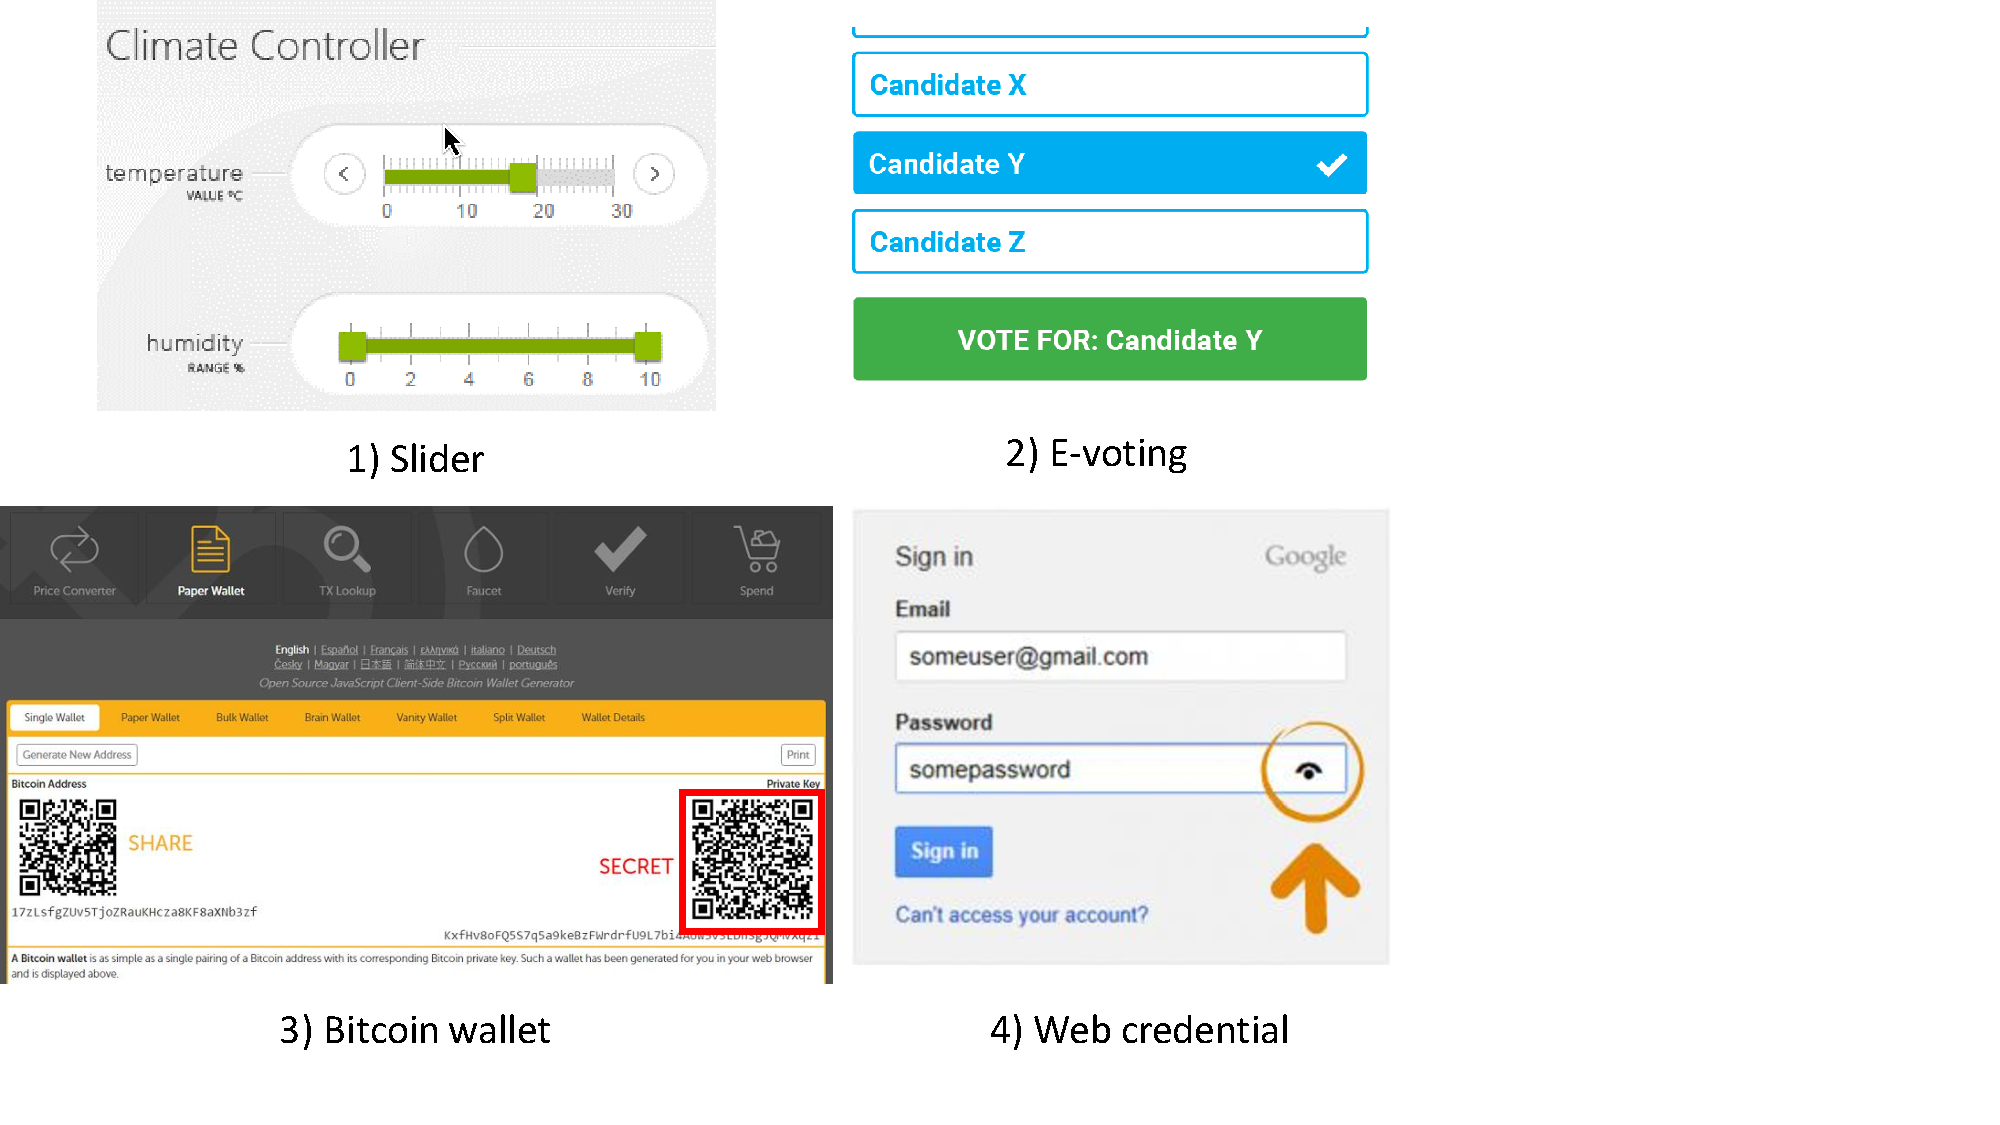
\includegraphics[trim={0 1cm 10cm 0}, clip, width=\linewidth]{motivation.pdf}
\caption{\textbf{Motivating examples.} 1) Pointer based UI elements that sets parameters to remote safety-critical device, 2) E-voting where the voting privacy and integrity is critical, 3) Financial transactions such as bitcoin wallet that shows sensitive information such as the user's private key and 4) web applications that provide an option for the user to reveal credentials.}
\spacesave
\label{fig:motivation}
\centering
\end{figure}


IO operation between the user and a remote server in the presence of an untrusted host is a long-standing problem. \emph{Trusted path} provides a secure channel between the user (HID) and the end-point where end-point is typically a trustworthy application running on the host. Trusted path ensures that input from the user is reached to the intended application, and all the outputs are generated by the legitimate application. Trusted path to the local host is a well-researched area where many solutions focus on using trusted software components such as a trusted hypervisor. In work done by Zhou et al.~\cite{zhou2012building}, the authors proposed a generic trusted path on $x86$ systems in pure hypervisor-based design. SGXIO~\cite{weiser2017sgxio} employed both the hypervisor and trusted execution environment (TEE) such as Intel SGX. Hypervisor requires too much TCB and often impractical in the real world scenario as most of the existing hypervisor offers very limited set of features.

However, when we consider an untrusted host, trusted path to the local host does not provide any advantage. In such an attacker model, it is crucial to ensure a trusted path from the user to a trusted remote server. Remote trusted path variant is non-trivial as typically all the IO operations are mediated by the operating system, device drivers, etc. To solve this problem, solutions typically rely on trusted external devices. Transaction confirmation devices~\cite{filyanov2011uni,weigold2011secure} allow the user to review her input data on a trusted device that is physically separated from the untrusted host but suffers from poor usability and is only limited to simple inputs. Bump in the Ether~\cite{McCPerRei2006} and IntegriKey~\cite{IntegriKey} uses external embedded devices to sign input parameters. However, such solutions ignore the view of the user context/view; hence, the attacker can execute UI manipulation attacks to trick the user into providing an incorrect input.

Out of the numerous works, Fidelius~\cite{Fidelius} provides the most comprehensive solution to protect keyboard inputs from a compromised browser using \red{additional devices and a} \js \red{interpreter} that runs inside an SGX enclave. Fidelius uses overlays on display, specifically on the input text boxes to hide sensitive user input from the browser. But Fidelius suffers from both security and functional issues. Fidelius does not provide output integrity, such as the integrity of the layout of the UI and the labels. This allows the attacker to change instruction on the screen to influence user such as changing the unit of an input value to a safety-critical device. The attacker can even trick the user into putting additional information that may compromise the integrity of the input data. Apart from such fundamental security problems, Fidelius is also vulnerable to  microarchitectural attacks on SGX enclaves~\cite{van2018foreshadow} that extracts the attestation keys, relay attack~\cite{dhar2018proximitee} that relays all user data to the attacker's platform, etc.
Also, Fidelius relies on an overlaid information bar that works as a passive security indicator. Several research works~\cite{egelman2008you,sobey2008exploring} show that in real-world, passive security indicators do not provide adequate security, and suffer from user habituation. From the functional point of view, Fidelius only supports keyboard input and text box as input UI.
 
 
\myparagraph{Our contribution} The shortcomings of the previous works provide the groundwork of our paper which shows that without output integrity, input integrity is not achievable. \name is built upon the idea of delivering input integrity by first ensuring output integrity. \name also eliminates the need for security indicator to eliminate the risk of user habituation. \name leverages a trusted low-TCB auxiliary device that we call \device that works as a generic IO hub between all user IO devices and the untrusted host. \device does not have any explicit network capability to communicate with the trusted remote server. Instead, the \device uses the host as an untrusted transport. \device ensures output integrity and confidentiality by sending an encoded UI to the host that only the \device can decode, and overlay on the display signal. The overlay is possible as the \device intercepts the display signal between the host and the monitor. The \device generated overlay ensures that the host can neither observe nor manipulate any output information; hence, it can not trick the user. The \device analyzes the intercepted HDMI frames to understand the correct user context, such as if the user moved her mouse over a specific UI element and click there. The \device also intercepts the mouse and keyboard signal and match them with the display signal that is received from the untrusted host. If both the input and output co-relates, the \device signs all the input and send them to the remote server. The signed input from the \device ensures input integrity and authenticity. \device is a fully plug-and-play device that is compatible with any host system regardless of their architecture and OS. We now summarize the contributions of \name as: 

%In our design of \name, the \device acts as the \emph{root-of-trust} as the mere fact of connecting all the IO devices to the \device ensures the IO security. 


\begin{mybullet}
  \item The primary contribution of this paper is to have the concrete understanding of the securing of user IO between the user and  a remote server that the related research works lack. Input integrity can only be achieved if output integrity is ensured. (Section~\ref{sec:approach})
  \item We describe the design of \name, a system that provides a remote trusted path from the server to the user, in an attacker-controlled environment. The design of \name leverages a small, low-TCB auxiliary device that acts as a \emph{root-of-trust} for the IO. \name protects the integrity and confidentiality of the UI, specifically the integrity of mouse pointer activities and of keyboard input integrity and confidentiality. \name is further designed to avoid user habituation. Unlike transaction confirmation devices, \name can be used to protect complex IO interaction that are common in today's web forms e.g., radio-button, drop-down menu etc. (refer to Section~\ref{sec:systemDesign} \&~\ref{sec:confidentiality}).
  \item We analyze the security of our solution in depth and argue why \name achieves IO integrity. We also discuss potential side channel leakages that may undermine the confidentiality of IO (refer to Section~\ref{sec:securityAnalysis}). 
  \item We also provide an prototype implementation of \name that is practical and easy to use (refer to Section~\ref{sec:prototype} \&~\ref{sec:eval}).
\end{mybullet}


\myparagraph{Organization of the paper} The organization of this paper is as the following. Section~\ref{sec:problemStatement} provides the detailed motivation, problem statement, state-of-the-art and the goals of this paper. Section~\ref{sec:approach} provides the system \& attacker model, challenges and a brief overview of our solution. We discussed the technical details of \name in Section~\ref{sec:systemDesign}. Section~\ref{sec:securityAnalysis} provides in-depth security analysis of \name. Section~\ref{sec:prototype} and~\ref{sec:eval} provide details of \name prototype implementation and corresponding evaluation. Finally, Section~\ref{sec:relatedWorks} and~\ref{sec:conclusion} provides the related research works and concludes the paper respectively.

%%%%%%%%%%%%%%%%%%%%%%%%%%%%%%%%%%%%%%
     %\myparagraph{State of the art} A trusted path provides roughly provide a set of four security properties to the communication channel between the user and the end system. Ensuring that the user performs intended actions to the remote server, typically, requires to assure that the user gets authentic output from the server. \emph{Output integrity} ensures that the information from the server reaches to the user in the intended form. For example, a user configuring a safety-critical device remotely bases her inputs in the current state of the system. As illustrated in the Figure~\ref{fig:motivation}, a compromised host could trick the user into performing unintended actions by providing incorrect feedback about the actual status. \emph{Output confidentiality} enables applications that require that the trusted paths offer a mechanism for the remote server to show secret information to the user. Figure~\ref{fig:motivation} illustrates such cases when a web server delivers a private key of a crypto-wallet to the user which should be kept hidden to the untrusted host.

%Once that output security is achieved, the trusted paths should guarantee that the remote servers accept only inputs generated by the honest user - \emph{Input integrity}. This feature is critical for the integrity of user actions in case of a compromised host. As shown in Figure~\ref{fig:motivation}, the user submits her inputs, and the remote server assures that a malicious host has not altered the user's original inputs. \emph{Input confidentiality} provides stricter security guarantees. Other applications (e.g., e-voting) require a higher level of security, the inputs should be sent to the server as generated by the user---input integrity---and preferably the host should not have access to inputs. Note that, to provide input security, trusted paths should guarantee at first output security.


%Trusted path is in focus in several recent research works. Several ways could be employed to realize the trusted path. For example, Filyanov et. al~\cite{filyanov2011uni} proposed transaction confirmation device that requires the user to use a separate device to confirm the input parameters. This allows the user to review her input data on a separate trusted device that is physically separated from the untrusted host. Trusted execution environments (TEE) such as Intel SGX, ARM TrustZone, TPM, Intel TXT, etc. provide isolated code execution, and can be used to achieve trusted path. Previous research works such as Intel SGX and trusted hypervisor-based SGXIO~\cite{weiser2017sgxio}, Intel SGX based ProximiTEE~\cite{dhar2018proximitee}, TPM and TXT based trusted path~\cite{filyanov2011uni}, and ARM TrustZone based trusted path~\cite{sun2015trustotp} are the example of trusted path construction based on TEEs. All of these solutions require specialized platforms with processors that support such infrastructure. VButton~\cite{li2018vbutton} uses ARM TrustZone to overlay buttons on the mobile devices that confirm if the user taps on a specific button. Processor-TEE such as Intel SGX primarily provides execution privacy and code integrity. In most of the cases, IO is still mediated by the OS. InContext~\cite{huang2012clickjacking} presents different clickjacking attacks variants and their solution by ensuring context (both temporal and visual) and pointer integrity in the trusted browser setting. Trusted hypervisors and secure micro-kernels are also choices for contrasting Trusted path. Sel4~\cite{klein2009sel4} is a functional hypervisor that is formally verified and has a kernel size of only $8400$ lines of code. In work done by Zhou et al.~\cite{zhou2012building}, the authors proposed a generic trusted path on $x86$ systems in pure hypervisor-based design. Examples of other hypervisor-based works can be found in systems such as Overshadow~\cite{Overshadow}, Virtual ghost~\cite{criswell2014virtual}, Inktag~\cite{hofmann2013inktag}, TrustVisor~\cite{mccune2010trustvisor}, Splitting interfaces~\cite{ta2006splitting}, $SP^3$~\cite{yang2008using}, etc.

%In spite of numerous existing research works on trusted path, none of the existing system provides an end-to-end secure trusted path that works on generic input devices, handles complex UI and user interactions, and introduces minimal or no changes to the existing systems and user's behaviour. This leads to the realization of our proposed solution, \name.


 
%\section{Background: Secure Web UI}
\label{sec:background}

The modern web browser provides a comprehensive set of mechanisms that protect users from malicious websites and \js, assuming that both the browser and the OS are trusted. W3C UI security specification \cite{w3c_spec} dictates such mechanisms. One known attack is the hidden element attack where the malicious \js renders an button-like object (could be a Facebook like) on top of another (could be a link to a malicious website) \red{where the former is transparent to click}. This tricks the user into clicking on the overlaid button, but the user is redirected to a malicious website. There exist several security policy directives to prevent such attacks. For example, \texttt{input-protection} directive enforces several input protection heuristics to protect users. \emph{Obstruction check} enables the browser to take screenshots of the screen area and to check if there is any overlaid element. Another heuristic is \emph{timing attacks countermeasure} where the browser maintains a list called \texttt{Display Change List} that contains all UI changes on the DOM tree. Using this list, the browser checks if there is any UI change on the security sensitive UIs. Developers can define \texttt{input-protection-clip} in the HTML which defines a rectangular screen area whose intersection with the bounding rectangle of the whole document's body should be used as the reference area in the screenshot comparison.

InContext~\cite{huang2012clickjacking} presents different clickjacking attacks variants and possible solutions to ensure context (both temporal and visual) and pointer integrity. In a clickjacking attack, a malicious \js renders a legitimate looking cursor on the browser. This fake cursor tricks the user into following that while the real cursor is on a sensitive UI element. InContext proposes a way to mitigate this attack by attracting the user attention when the actual cursor is on a security-sensitive UI. Focusing user attention could be done by several means. Lightbox mechanism allows the browser to gray out the rest of the part of the screen except the security-sensitive UI element when the real cursor enters the UI. Freezing makes the portion of the frame suspended when the user enters the sensitive UI. %The browser also enforces a time delay of clicking on a sensitive button to allow a cool-down period.  
\section{Problem Statement}
\label{sec:problemStatement}

In this section, we motivate our work in the context of securing user's IO to remote servers. We also describe selected existing literature that tackles the relevant problem, and we discuss how those works lack proper solution and how our solution is different from them. Lastly, we explain the goals of our work.

\subsection{Motivation: Secure IO with Remote Safety-critical System}

A user communicates with a remote server through a host, which gives the host access to the plaintext IO data that is exchanged between the user and the remote server. The host consists of large and complex system software such as the modern operating systems, device drivers, etc., applications such as browser, and diverse set of hardware components expose the host to a large attack surface. An adversary that controls the user's host can alter user intentions, i.e., it can perform arbitrary actions on behalf of the user, modify the input parameters, or show wrong information to the user. Such an adversary is very powerful and difficult to be detected or prevented by a remote server. The consequences of such attacks might be severe when safety-critical applications are targeted. The attacker can pass the wrong input to a remote safety-critical system such as a medical device, power plant, etc.

Trusted execution environments (TEEs) enable remote trust into the code executing on the processor, effectively eliminating the need to trust more significant code base (motherboard, memory modules, OS and other applications). Processor TEE such as Intel SGX relies on the OS to mediate all the user IO. Hence, the problem of isolating user's input and output remains. Therefore, service providers typically operate with the assumption that the data they receive is genuine (generated by the user) and not altered by a compromised host. However, system-level TEEs such as ARM TrustZone makes the job of securing the IO easier as one can implement privileged code like IO drivers inside the trusted environment. This is not possible in TEE architectures like SGX. But such a mechanism is limited to ARM platforms, making them infeasible for \emph{x86} platforms. Despite such features, usability issues such as security indicators, relying on secure boot, etc. to ensure IO integrity and confidentiality remain.


\begin{figure}[t]
\centering
%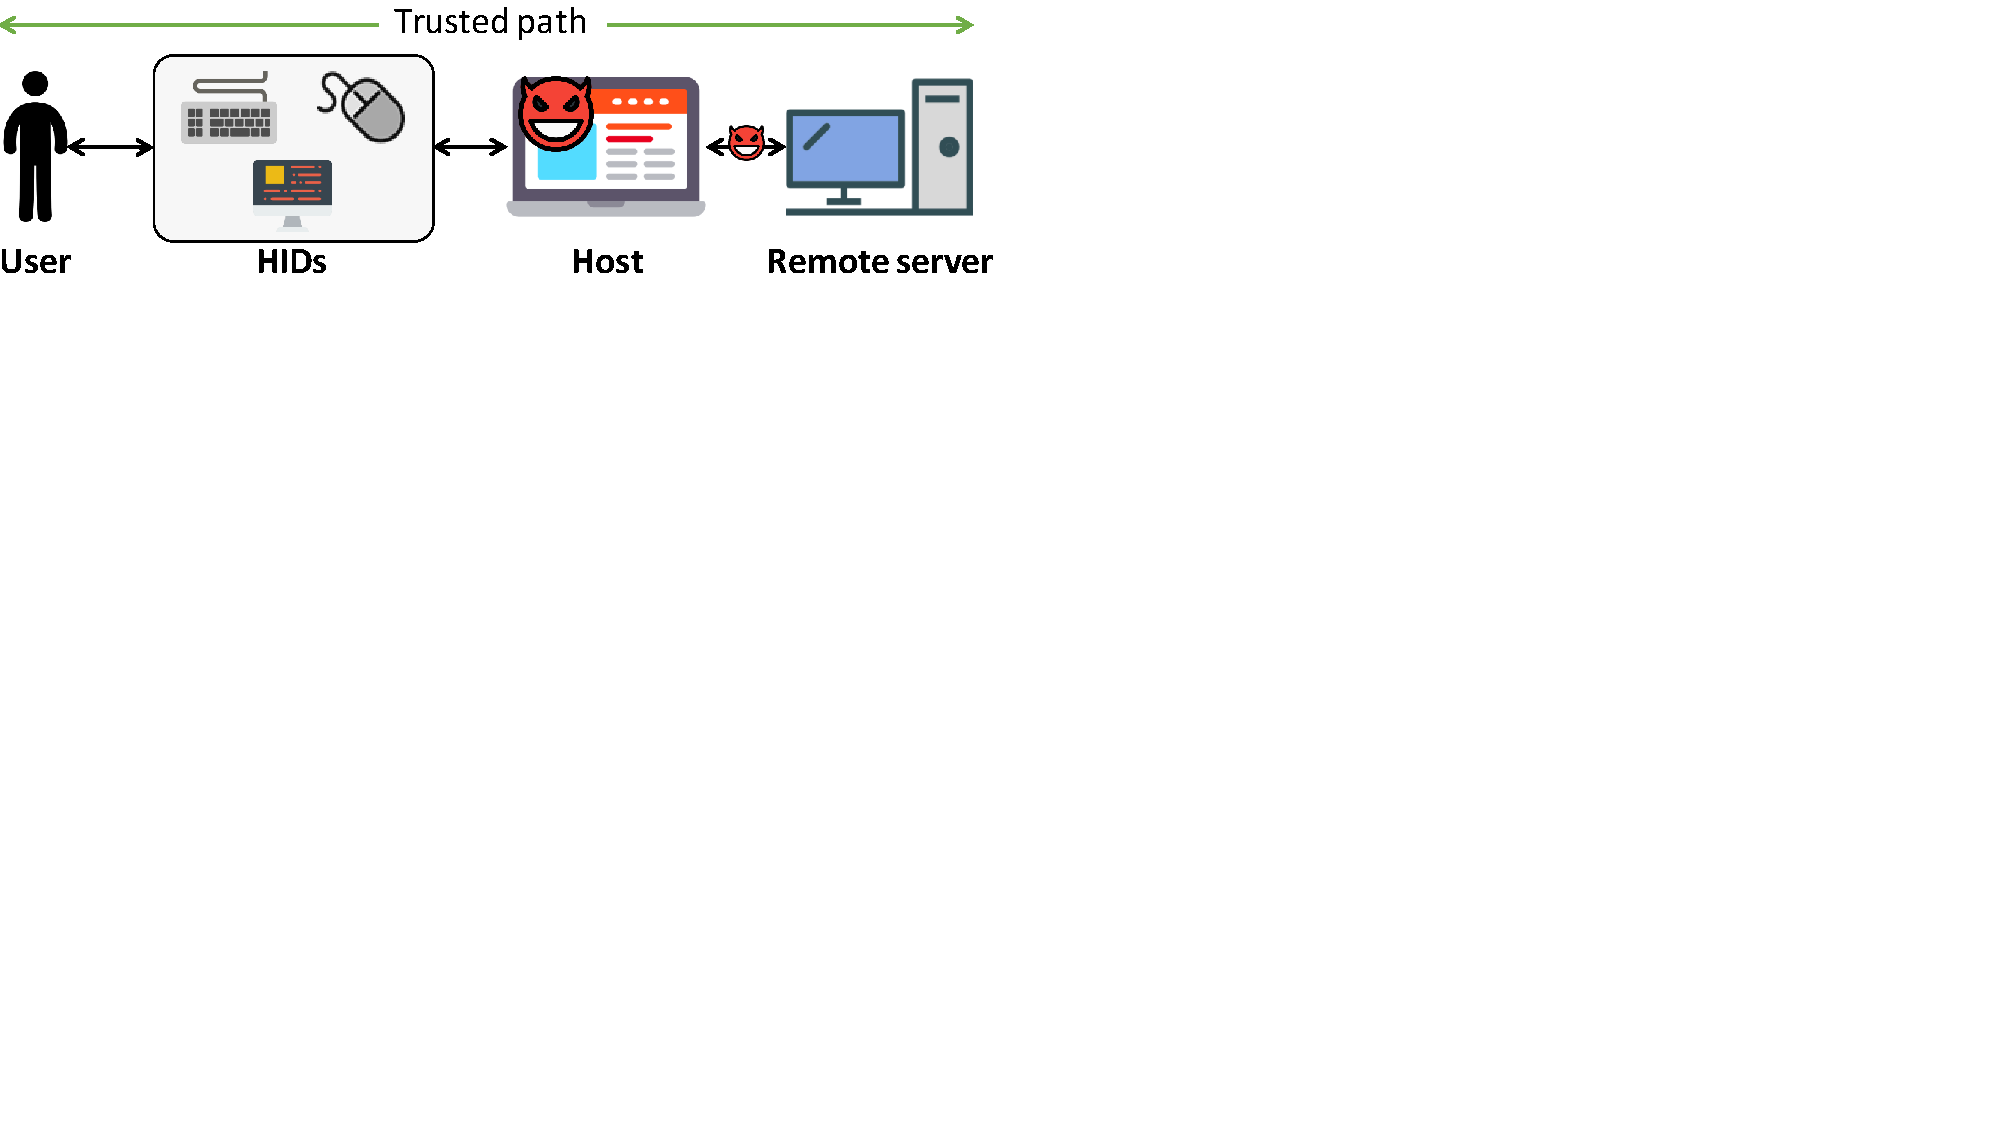
\includegraphics[trim={0 14cm 17cm 0}, clip, width=0.9\linewidth]{systemModel.pdf}
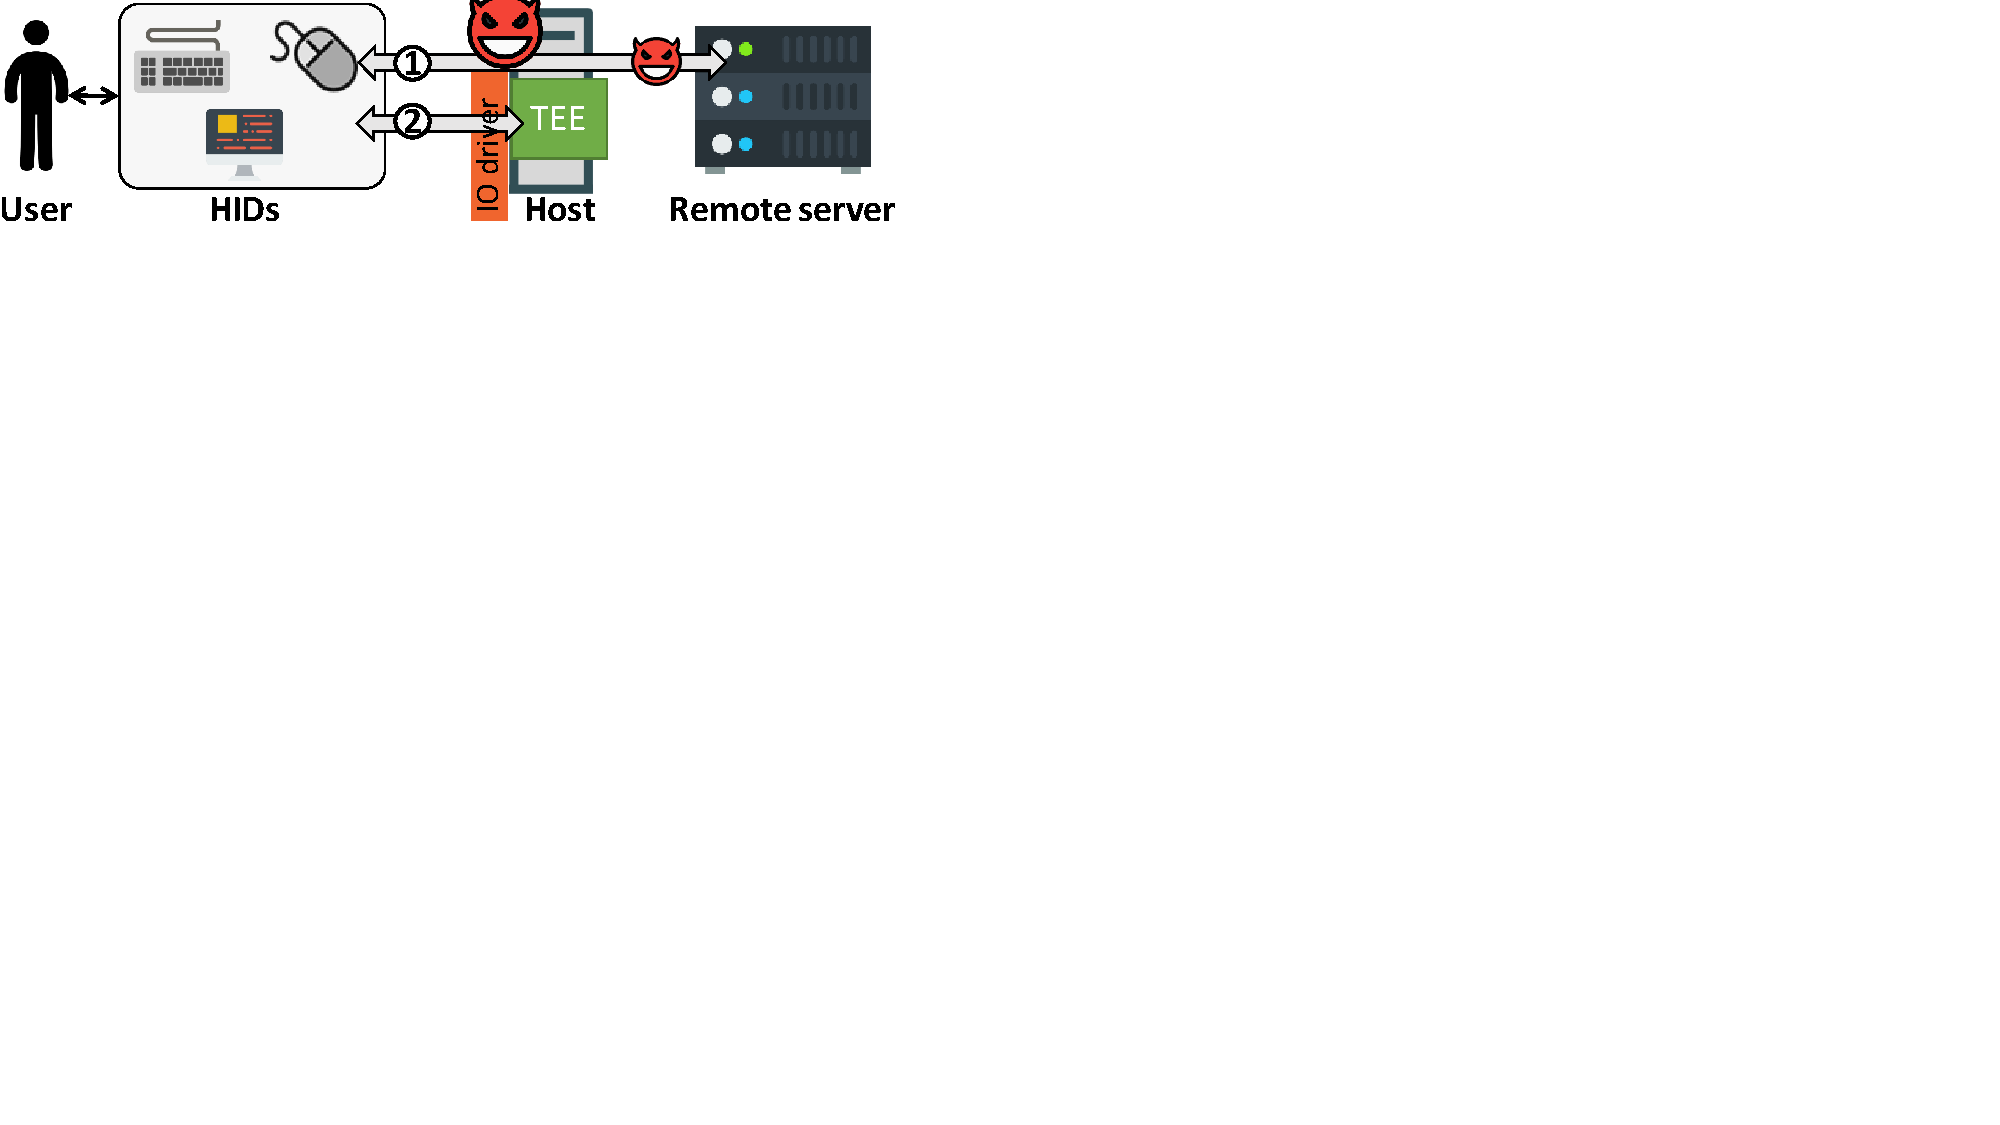
\includegraphics[trim={0 15cm 18cm 0}, clip, width=0.9\linewidth]{systemModel_all.pdf}
\caption{\textbf{Trusted path.} The figures shows the system and the attacker model of the trusted path. We generally consider two trusted path scenarios, \one trusted path to a remote server, and \two trusted path to a trusted execution environment (TEE) such as the Intel SGX.}
\spacesave
\label{fig:trustedPath}
\centering 
\end{figure}

In a traditional settings. a \emph{Trusted path} provides a secure channel between the user and a trusted application running on the location host. Trusted path allows the user to ensure that her input is reaching to the intended application rather than a malicious one and the output is generated by the legitimate application. However, in the setting where the local host is fully compromised, trusted path to the local host does not provide any advantage, except is the local host supports TEE and runs an isolated enclaves on the local host. However, establishing a trusted path to a remote server is non-trivial as the IO data is mediated by the untrusted operating system. Figure~\ref{fig:trustedPath} shows two different scenarios where the trusted path extends from user IO devices to \one a remote server, and \two a local enclave. %In principle, a trusted path solves the general security problem of the IO data. 
%But practically establishing a trusted path in general IO devices is a nontrivial problem specifically if one considers the plethora of complex UI objects and input methods as well as different security and functional properties that a solution should satisfy. 
In this paper, we primarily target the trusted path problem to a remote server (such as a remote PLC, web server or remotely accessible medical device, etc.) accessing from a commodity $x86$ host.

\iffalse
\subsection{Security Properties}

A \emph{Trusted path} provides confidentiality and integrity to the IO data exchanged between the users and the end systems. In principle, a trusted path solve the general security problem of the IO data. But practically establishing a trusted path in general IO devices is a nontrivial problem specifically if one considers the plethora of complex UI objects and input methods as well as different security and functional properties that a solution should satisfy. We list these properties below. 


\begin{mylist}
  \item \textbf{Input integrity and confidentiality.} These properties define that any input that is coming from the user input devices are fully protected in two ways: i) the input issued by the user reaches to the remote end-point as it was generated by the user - \emph{integrity}, and ii) in specific application scenarios, the attacker-controlled host is entirely oblivious about the input from the user - \emph{confidentiality}. The trusted path system should consider a wide range of input devices, such as keyboard, mouse, touch, etc. We consider any sort of input action by the user that may include moving the mouse or using the keyboard navigation keys to select a specific item in a list.
  
  
  \item \textbf{Output integrity and confidentiality.} Similar to the input integrity, output integrity ensures that information that is sent by the remote endpoint is presented to the user as it was meant to be. One example of output integrity is the integrity of the UI elements. Such property ensures that the host system renders the UI elements faithfully as they were sent by the remote system. Output confidentiality ensures that the information sent by the remote server can not be accessed by the attacker-controlled host. 
  
 %  \item \textbf{Usability.} The trusted path should neither change the typical user interaction with a computer nor should require extensive changes into the existing systems.

  As discussed on the Section~\ref{sec:securityAnalysis}, ensuring output integrity is essential for providing input integrity against advanced attackers that trick the user into sending non-legitimate data to the server. For example, the user wants to send a number \texttt{10} to the server, but the malicious host shows on screen \texttt{100} and fools the user into believing he mistyped a \texttt{0}. The user deletes one \texttt{0} and sees \texttt{10} on the screen---as he intended initially---and submits the data, however, on the server arrives just \texttt{1}. 
  
  Providing output integrity is a challenging task even on systems that have a trusted component that overlays parts of the HDMI frames generated by the untrusted host. Previous works~\cite{huang2012clickjacking} show that when a trusted component and an untrusted one share a screen, the attacker can still manipulate the user to commit unintentional actions to the trusted UI if the system is not designed properly. In our solution we want to guarantee that the user is aware of the UI elements (trusted or untrusted) that she interacts with, therefore preventing related attacks.
  \end{mylist}

\fi




\subsection{Existing Solutions and their drawbacks}

\iffalse
\begin{figure}[t]
\footnotesize
    \centering
    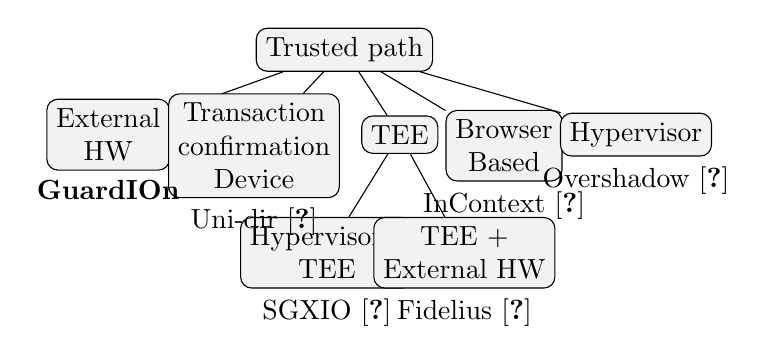
\begin{tikzpicture}[
solved/.style={rectangle,draw,fill=purple!40, rounded corners, align=center},
not/.style={rectangle, draw,fill=orange!60, rounded corners, align=center},
neutral/.style={rectangle, draw, rounded corners, align=center, fill=black!5}
]]
    \node[neutral](root) {Trusted path}
    child { node[neutral, yshift=12pt] (hw) {External\\ HW}}
    child { node[neutral, yshift=8pt, xshift=10pt] (tc) {Transaction\\ confirmation\\ Device}}  
    child { node[neutral, yshift=12pt, xshift=20pt] (tee) {TEE}
      child { node[neutral, yshift=0pt, xshift=-5pt] (teehv) {Hypervisor+\\TEE}}
      child { node[neutral, yshift=0pt, xshift=2pt] (teehw) {TEE + \\ External HW} } }
      child { node[neutral, yshift=8pt, xshift=15pt] (br) {Browser\\ Based}}   
     child { node[neutral, yshift=12pt, xshift=20pt] (hv) {Hypervisor}}  ;
    
    \node[below=0cm of hw] {\textbf{\name}};
    \node[below=0cm of tc] {Uni-dir~\cite{filyanov2011uni}};
    \node[below=0cm of hv] {Overshadow~\cite{Overshadow}};
    \node[below=0cm of teehv] {SGXIO~\cite{weiser2017sgxio}};
    \node[below=0cm of teehw] {Fidelius~\cite{Fidelius}};
     \node[below=0cm of br] {InContext~\cite{blake1998authenticated}};    
    \end{tikzpicture}
    
   \caption{\textbf{Summarization of existing trusted path solutions} by their approach. A detailed description of the related works is discussed in Table~\ref{tab:relatedWorks}.}
     \label{fig:relatedWorksTree}
\end{figure}
\fi

\newcommand{\relatedWorkTree}
{\begin{figure}[t]
\footnotesize
    \centering
    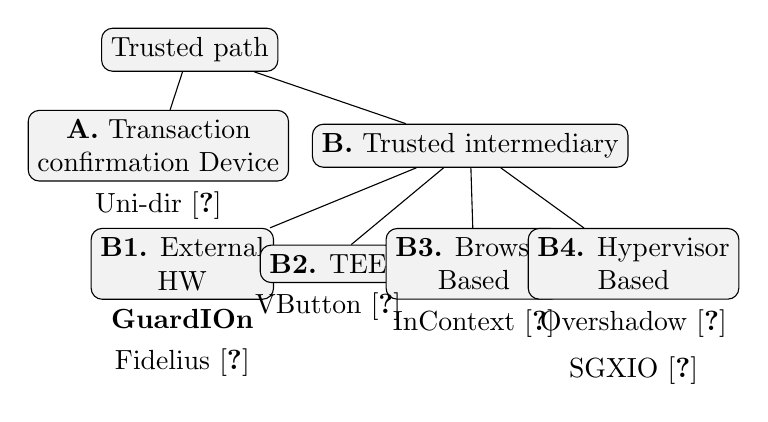
\begin{tikzpicture}[
solved/.style={rectangle,draw,fill=purple!40, rounded corners, align=center},
not/.style={rectangle, draw,fill=orange!60, rounded corners, align=center},
neutral/.style={rectangle, draw, rounded corners, align=center, fill=black!5}
]]
    \node[neutral, xshift=10pt](root) {Trusted path}
    child { node[neutral, yshift=8pt, xshift=10pt] (tc) {\textbf{A.} Transaction\\ confirmation Device}}  
    child { node[neutral, yshift=8pt, xshift=80pt] (td) {\textbf{B.} Trusted intermediary}
        child { node[neutral, yshift=0pt, xshift=-40pt] (hw) {\textbf{B1.} External\\ HW}}
        child { node[neutral, yshift=0pt, xshift=-30pt] (tee) {\textbf{B2.} TEE}}
      child { node[neutral, yshift=0pt, xshift=-20pt] (br) {\textbf{B3.} Browser\\ Based}}   
     child { node[neutral, yshift=0pt, xshift=-5pt] (hv) {\textbf{B4.} Hypervisor\\ Based}} 
    }    ; 
      

    \node[below=0cm of hw](gurdion) {\textbf{\name}};
    \node[below=0cm of tee] {VButton~\cite{li2018vbutton}};
    \node[below=0cm of tc] {Uni-dir~\cite{filyanov2011uni}};
    \node[below=0cm of hv](os) {Overshadow~\cite{Overshadow}};
    \node[below=0cm of os] {SGXIO~\cite{weiser2017sgxio}};
    \node[below=0cm of gurdion] {Fidelius~\cite{Fidelius}};
     \node[below=0cm of br] {InContext~\cite{blake1998authenticated}};

    
    \end{tikzpicture}
    
   \caption{\textbf{Summarization of existing trusted path solutions} by their approach. A detailed description of the related works is discussed in Table~\ref{tab:relatedWorks} in Appendix~\ref{appendix:sec:summaryResearch}.}\spacesave
     \label{fig:relatedWorksTree}
\end{figure}
}

There exist two broad categories of existing solutions that try to solve the problem of trusted paths for IO devices in the presence of a compromised host: A) Solutions where unprotected user interaction first happens and then a trusted component (transaction confirmation device) is used to double check that manipulation did not happen, and B) Solutions where a trusted component that can capture user's input/output and then securely mediate it to the destination. The trusted component can be a browser, hypervisor, external hardware, etc. %But all of these solutions targeted for different problem settings and models. 
Figure~\ref{fig:relatedWorksTree} provides a board classification of the related works and illustrates where our proposed work stands concerning them. %We can generally classify the work into two broad categories based on the trusted path approaches transaction confirmation device and existence of other trusted components.

\myparagraph{A. Transaction confirmation devices} In their paper, Filyanov et. al~\cite{filyanov2011uni} proposed transaction confirmation device that requires the user to use a separate device to confirm the input parameters. The transaction confirmation suffers from three significant drawbacks. The first drawback is risk of \emph{user habituation}. Transaction confirmation device introduces lots of cognitive load over the user and may force the user to confirm their action without even looking to the input data. The second \emph{usability}, i.e., interacting with a small device can be cumbersome. Such user action makes the transaction confirmation device impractical in day-to-day interactions. Finally \emph{simple UI}, i.e., transaction confirmation is not practical/suitable for complex interaction, rather simple text-based inputs. 

%In contrary, \name supports generic input devices and supports complex user interfaces and user interactions. Moreover, the complete automated nature of \name does not introduce any cognitive load on the user, making the system less susceptible to user error.

\relatedWorkTree

\myparagraph{B1. External hardware-based solution}  Also known as the bump in the wire~\cite{McCPerRei2006}. Fidelius~\cite{Fidelius} uses raspberry pi's and Intel SGX to create a secure channel between the keyboard and the display device. By doing so, Fidelius provides secure input and display for the character-based device - keyboard. Additionally, Fidelius uses overlays to hide the keyboard input from the compromised host so that the input is only visible to the user. Fidelius only tackles keyboard-based input and utilizes SGX that separates Fidelius and \name in terms of the trust assumption. Systems such as ZTIC~\cite{weigold2011secure} uses external device with display and smartcard attachment to confirm inputs. Android OS also provide similar~\cite{android_confirm} mechanism to confirm protected transactions.
%None of these works looked into complex user interactions such as mouse movement or complex user interfaces. 


\myparagraph{B2. Trusted Execution Environments} TEEs specifically system TEEs such as ARM TrustZone is used in the literature to implement a trusted path between the IO devices and the users. %Several TEEs such as Intel SGX, ARM TrustZone, TPM, Intel TXT, etc. can be used to achieve such functionality.  
VButton~\cite{li2018vbutton} leverages ARM TrustZone to overlay buttons on the mobile device to confirm if the user taps on a specific button. Our solution is fundamentally different from VButtion as i) VButtion is specifically tuned for mobile devices, employing ARM TrustZone whereas our solution is more generic and targets specifically PCs, and ii) mouse input is significantly different than touch-based input as mouse input involves continuous movement where the touch or taps are discrete events. In this paper, we concentrate on the non-specialized hardware platform where compatible TEE technologies such as ARM TrustZone may not be available, e.g., x86 architecture. 
%Intel SGX based trusted path such as BastionSGX~\cite{BASTION-SGX} implements a trusted Bluetooth application inside an Intel SGX enclave to establish a trusted path between the keyboard and mouse and the SGX. But lack of output integrity makes the system unreliable as the paper failed to address how to transfer the mouse data reliably to the user and the remote server. 

\myparagraph{B3. Browser-based solutions} InContext~\cite{huang2012clickjacking} presents different clickjacking attacks variants and their solution by ensuring context (both temporal and visual) and pointer integrity. The trust model is significantly different from our work as it assumes that the browser and the OS are trusted. This makes the InConext i) not directly compatible with the attacker model that \name targets, and ii) targets a specific attack scenario (clickjacking vs. generic trusted path).


\myparagraph{B4. Trusted hypervisor-based solutions} Trusted hypervisors and secure micro-kernels are also alternatives to achieve Trusted path. In work done by Zhou et al.~\cite{zhou2012building}, the authors proposed a generic trusted path on $x86$ systems in pure hypervisor-based design. Solutions such as SGXIO~\cite{weiser2017sgxio}  combine a TEE and a hypervisor to mitigate the shortcomings of TEEs like SGX (i.e., the IO operations are handled by the OS). One major drawback of such solutions is the trust assumption that involves a full hypervisor. One can argue that a hypervisor that provides a rich set of functionalities has code base size of an OS. Second, most of the minimal hypervisor also does not offer common usable features such as rich IO, UI, etc., making them impractical for day-to-day usage in consumer devices. %\name avoids such extensive trust assumptions and assumes that the entire host is in control of the attacker.

%There exist several works that use TEE and hypervisor simultaneously to mitigate the shortcomings of TEEs like SGX (i.e., the IO operations are handled by the OS). Existing research such as SGXIO~\cite{weiser2017sgxio} requires the IO drives to be implemented inside the TEE or using trusted hypervisor that extends the size of the TCB significantly. Moreover, TEE requires trust assumption on the processors and additional code bases. One such example is Intel SGX where the trust model includes the physical processor package, SGX SDK, quoting enclave, launch enclave and Intel attestation service. Our proposed solution avoids such extensive trust assumptions and assumes that the entire platform is in control of the attacker.



%In summary, even though, there exist several research works that look into the problem of the trusted path, none of them provide a complete, secure, practical and usable trusted path solution. In our knowledge, \name incorporates all the features together for the first time: complex user interactions and UI elements, generic IO devices and low overhead on the user interactions. All of these are achieved in the smallest trust assumption.  

%Note that the majority of the previous works achieve some form of trusted path specifically for keyboard-based input. However supporting mouse and touch-based input, complex and generic user interfaces and protected users' action (such as the movement of the mouse pointer, gestures, etc.) in a security-sensitive application (such as e-voting) is not a trivial task. Without proper analysis of every frame that the host system produces, it is not possible to track user intention. In our knowledge, our proposed solution is the first to provide such security properties including the confidentiality of user input (e.g., mouse movement). Moreover, we want to achieve this in the absence of any TEE as the trust model of our scenario is significantly different.

%Detailed description of the related research is described in Table~\ref{tab:relatedWorks} in Appendix~\ref{sec:summaryResearch}.

\subsection{Goals}
\label{sec:problemStatement:goals}

In the above, we discussed several solutions and research works that solve the problem of constructing a trusted path in different ways. What makes our solution different from them is the specific attacker model and the end goals that it targets.
%We do not assume trust in the OS, particular drivers, TEEs, hypervisors, etc. As all of these techniques as mentioned earlier require trust on a large code base. Instead, our proposed solution solves the problem of building an efficient, trusted path using an off-the-shelf microcontroller and single board computers that require a bare-minimum trust assumption. The most distinguishing factor is the type of IOs our proposed system targets to protect, namely mouse/touch inputs and sophisticated user interfaces. Existing research works primarily targets character-based input devices such as keyboards, and the methods cannot be trivially applied to mouse/touch-based inputs or complex UI elements. 
The general goals of this paper are the following:

\begin{mylist}
  \item  \textbf{Rich set of IO security features.} Most of the existing trusted path solutions focus on a minimal set of feature (e.g., only support for keyboard). The primary goal of \name is to be compatible with generic IO device (such as a keyboard, mouse, touch screen, display, etc. in x86 architecture), and to provide integrity and confidentiality to all IO. 
  
  \item  \textbf{Small trust assumption.} Our goal is to provide the aforementioned rich set of IO and security features with minimal trust assumption that does not rely on a specialized hypervisor or a trusted OS. %Rather \name only trust a plug-and-play small-TCB trusted device that is made out of off-the-shelf components.  
  
  \item \textbf{Easy to deploy.} Our goal is also to provide a solution that comes with low deployment overhead such as a plug-and-play device that uses off-the-shelf components and the solution is compatible with any platform (OS, processor architecture, etc.). 
  
  \item \textbf{Usage safety.} Moreover, our goal is not to change the way users interacts with UI elements and imposing no or minimal cognitive load such as eliminating the need to see an external device to confirm a transaction, looking to a security indicator and confirming actions, etc. By doing so, we do not risk user habituation. 

\end{mylist}

In the following section what follows is the \name's design and how \name achieves these goals.

\section{\name Approach Overview}
\label{sec:approach}


\begin{figure}[t]
\centering
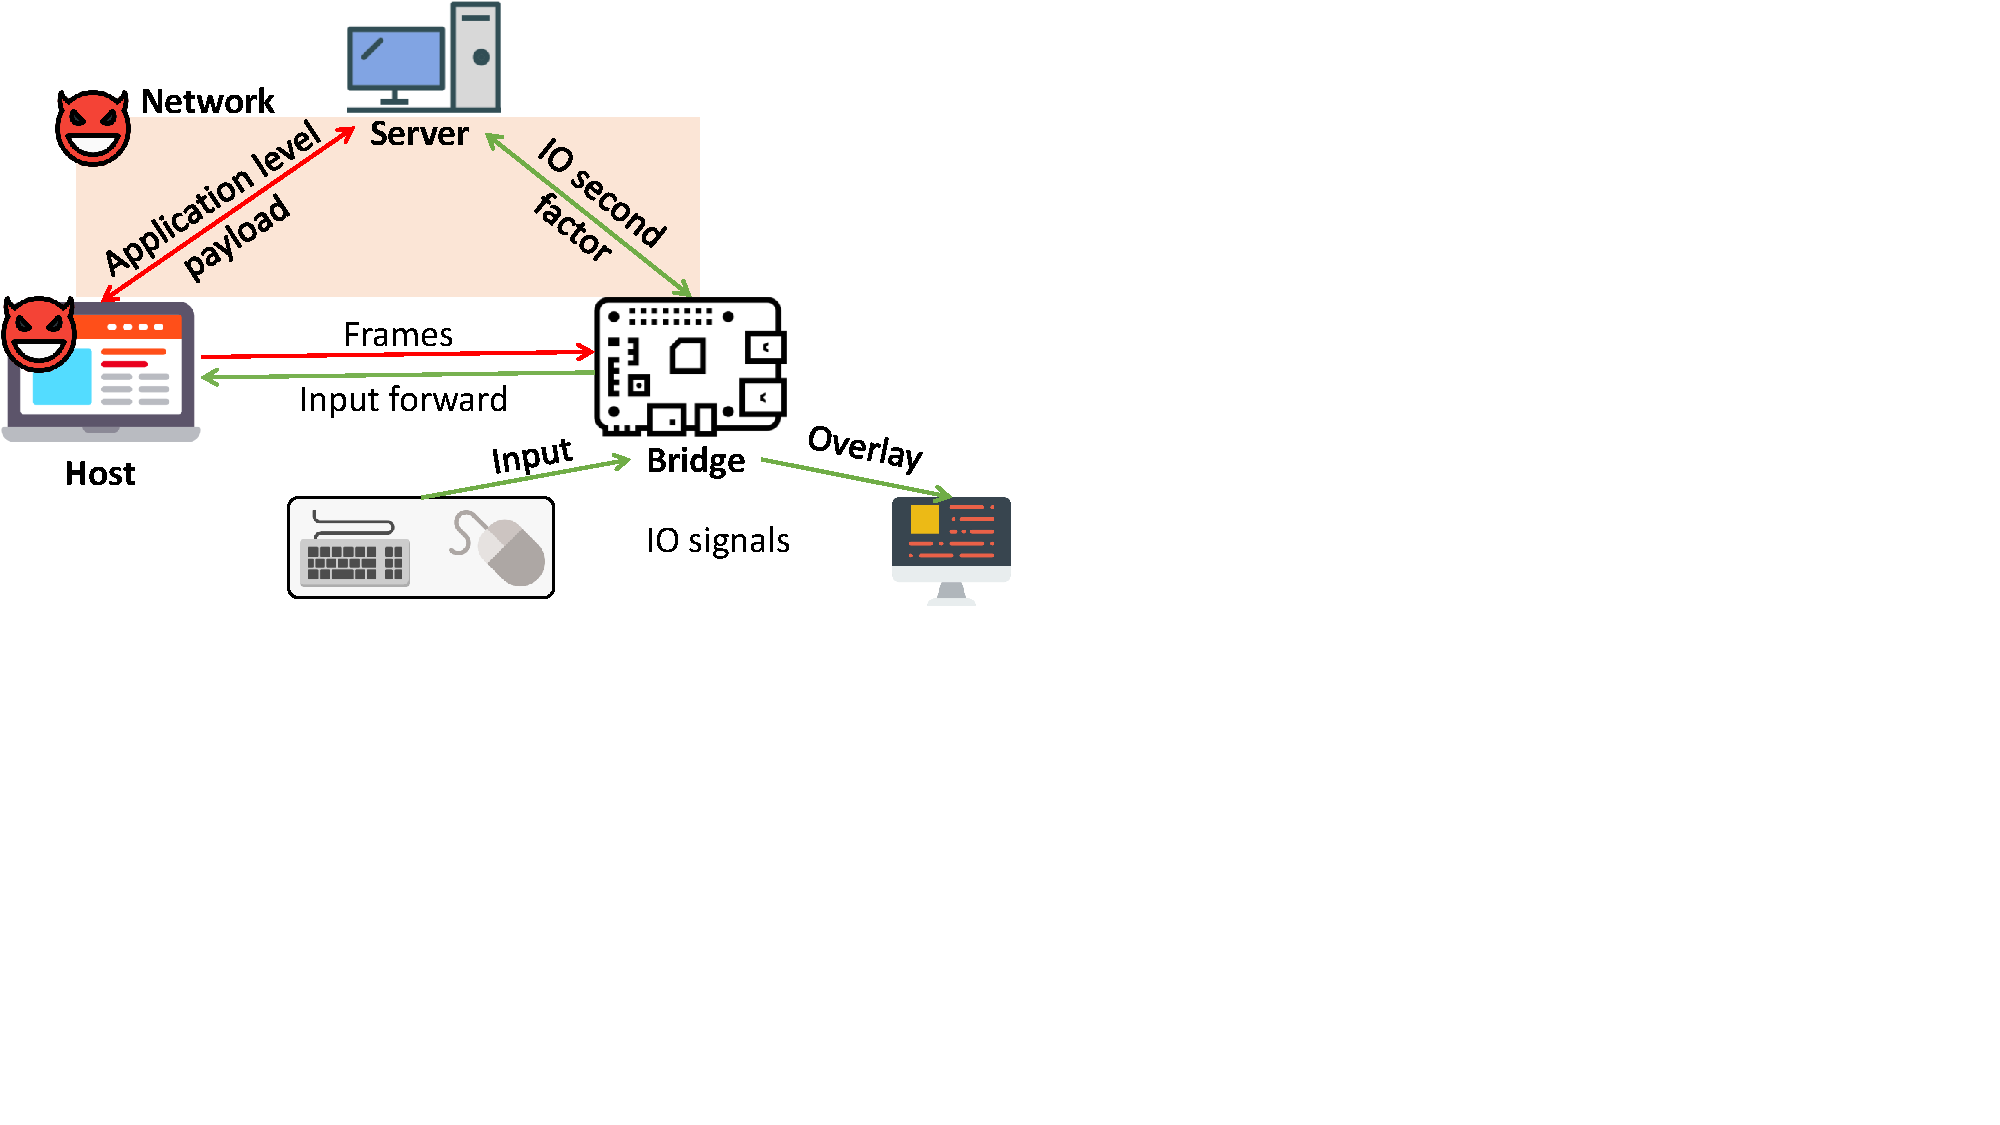
\includegraphics[trim={0 6cm 17cm 0}, clip, width=0.85\linewidth]{approachOverview.pdf}
\caption{\textbf{High-level approach overview of our solution.}  The \device connects the IO devices and the attacker-controlled host. }
\label{fig:approachOverview}
\centering
\end{figure}


In this section, we describe an overview of our proposed solution. As described in the problem statement discussed in Section~\ref{sec:problemStatement}, our proposed solution provides a trusted path between the user IO device and the remote server by utilizing a trusted embedded device as a mediator between all the IO devices and the untrusted host. We call this device: \device. The approach, on the high-level, uses the concept of the \emph{bump in the wire}~\cite{McCPerRei2006} to provide integrity and privacy to the user IO actions. The overall approach is illustrated in Figure~\ref{fig:approachOverview}. On a high level, the remote server and the \device establish a secure channel using the untrusted host as a transport. Note that the \device does not have any network capabilities, instead uses the host as an untrusted transport. The server also adds a small JavaScript snippet that allows the \device and the remote server to communicate. This eliminates any need for additional hardware/software aids on the user's machine.

We first define the system and attacker model, then outline the challenges and the brief outline of our proposed solution.

%Given the problem statement discussed in Section~\ref{sec:problemStatement}, we first define the attacker model we consider in our proposed system.


\subsection{System and Attacker Model}

We consider a system model where the user wants to send the input to a safety-critical remote end-system. The model is depicted in Figure~\ref{fig:approachOverview} that shows the compromised host, remote server and the user IO devices. 

We assume that the attacker compromises the host system completely (OS, installed applications and hardware). The attacker also controls the network. We assume that the attacker is a probabilistic polynomial time (PPT) algorithm that can not break crypto. Figure~\ref{fig:systemModel} shows the components of the system that are controlled by the attacker, i.e., the host and the network communication channel between the host and the remote server.

We only assume that the monitor, keyboard, mouse (in a word all the IO devices that we need to protect from the malicious host) and the \device are trusted, which is not unrealistic. The monitor, keyboard, and mouse have hardly any complex hardware. The TCB\footnote{Is this the TCB of the system or IO devices?} is very small.

\iffalse
\begin{figure}[t]
\centering
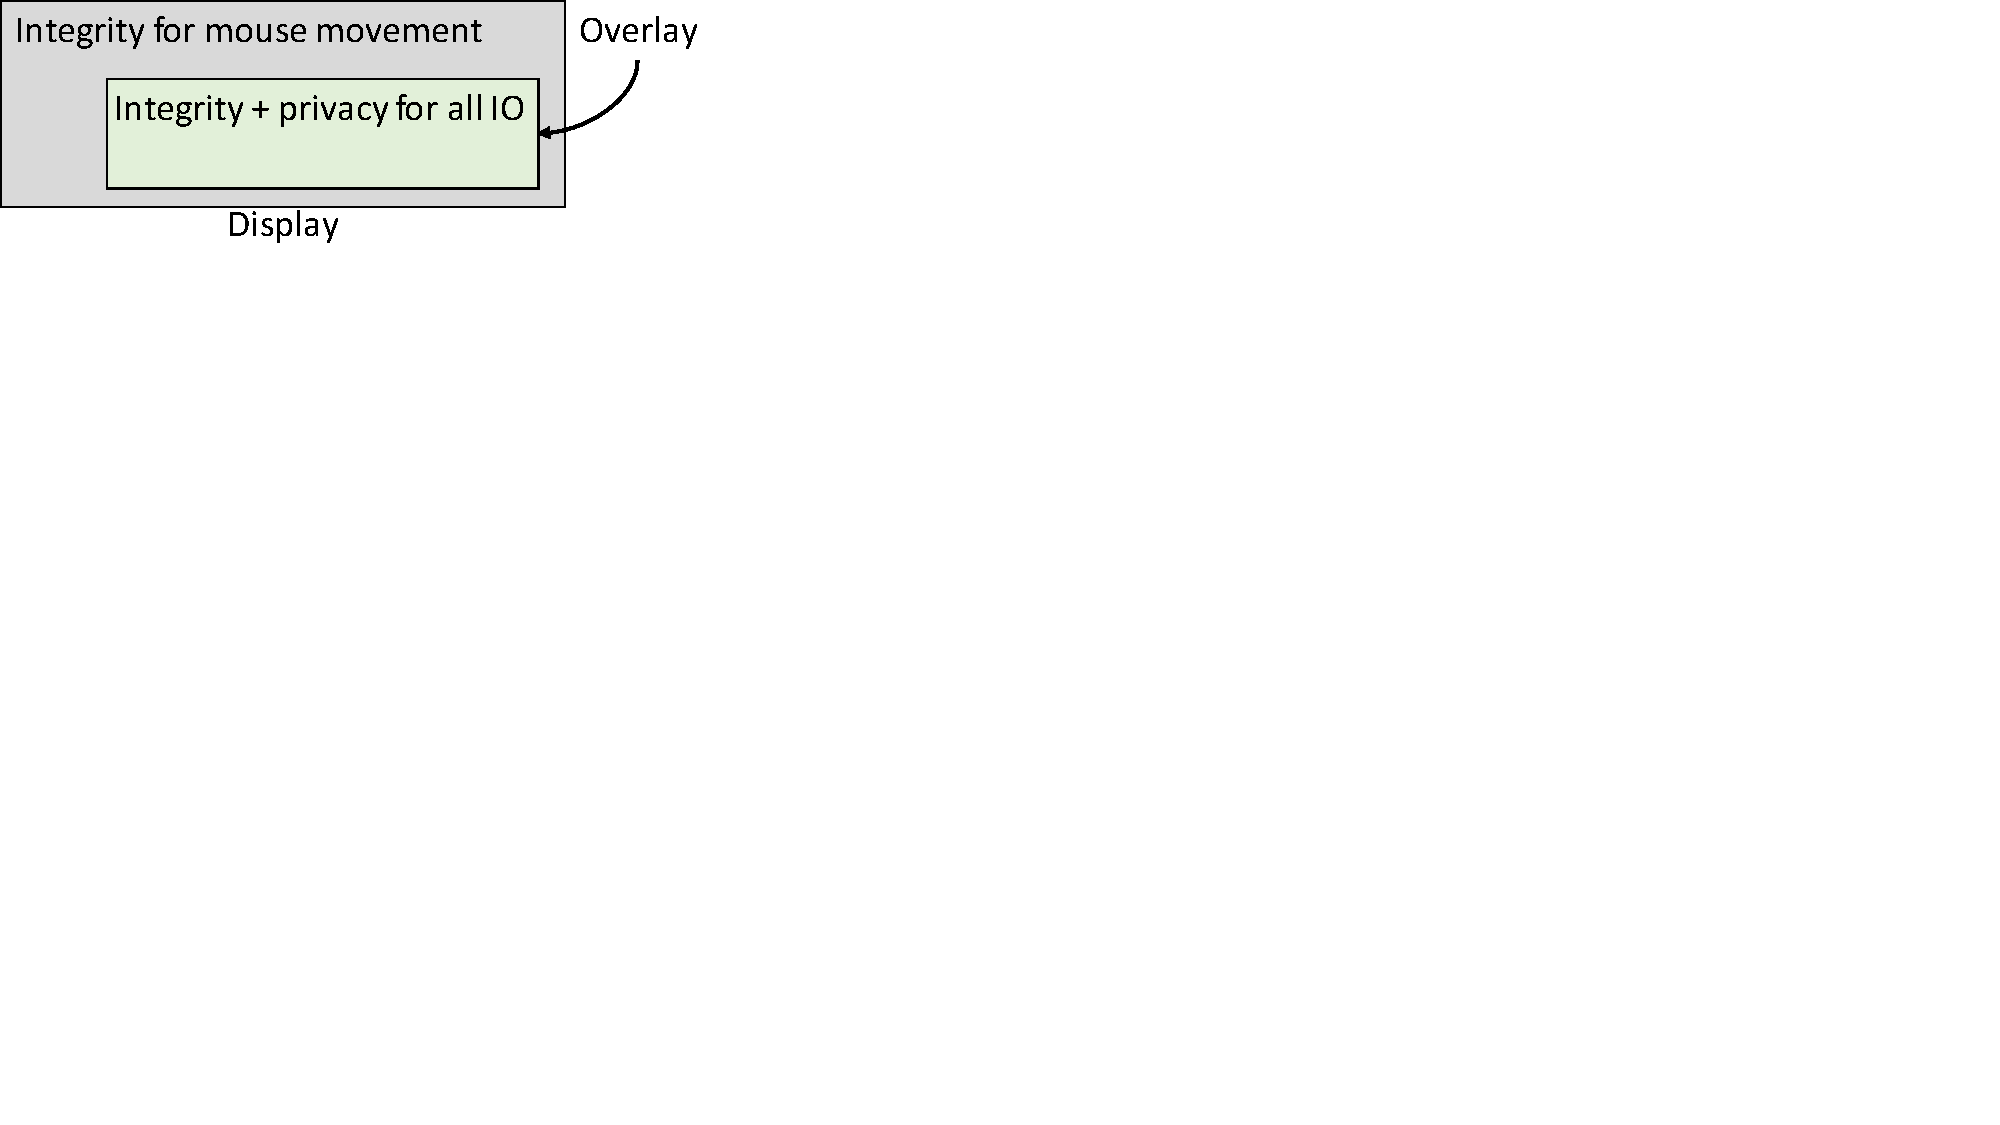
\includegraphics[trim={0 13cm 21.7cm 0}, clip, width=0.65\linewidth]{screenPartition.pdf}
\caption{\textbf{\device's pointer tracking, pointer \& UI overlay, and security properties.} Our proposed method provides two layers of protection for IO to the user. 1. In all the parts of the screen, the \device provide pointer integrity (the gray part). 2. The green part of the screen where the \device overlays on the HDMI stream where the \device provide integrity and privacy (privacy is dependent on the application requirements) for the IO.}
\label{fig:screenPartition}
\centering
\end{figure}
\fi



\subsection{High-level Description of the System}

\begin{figure}[t]
\centering
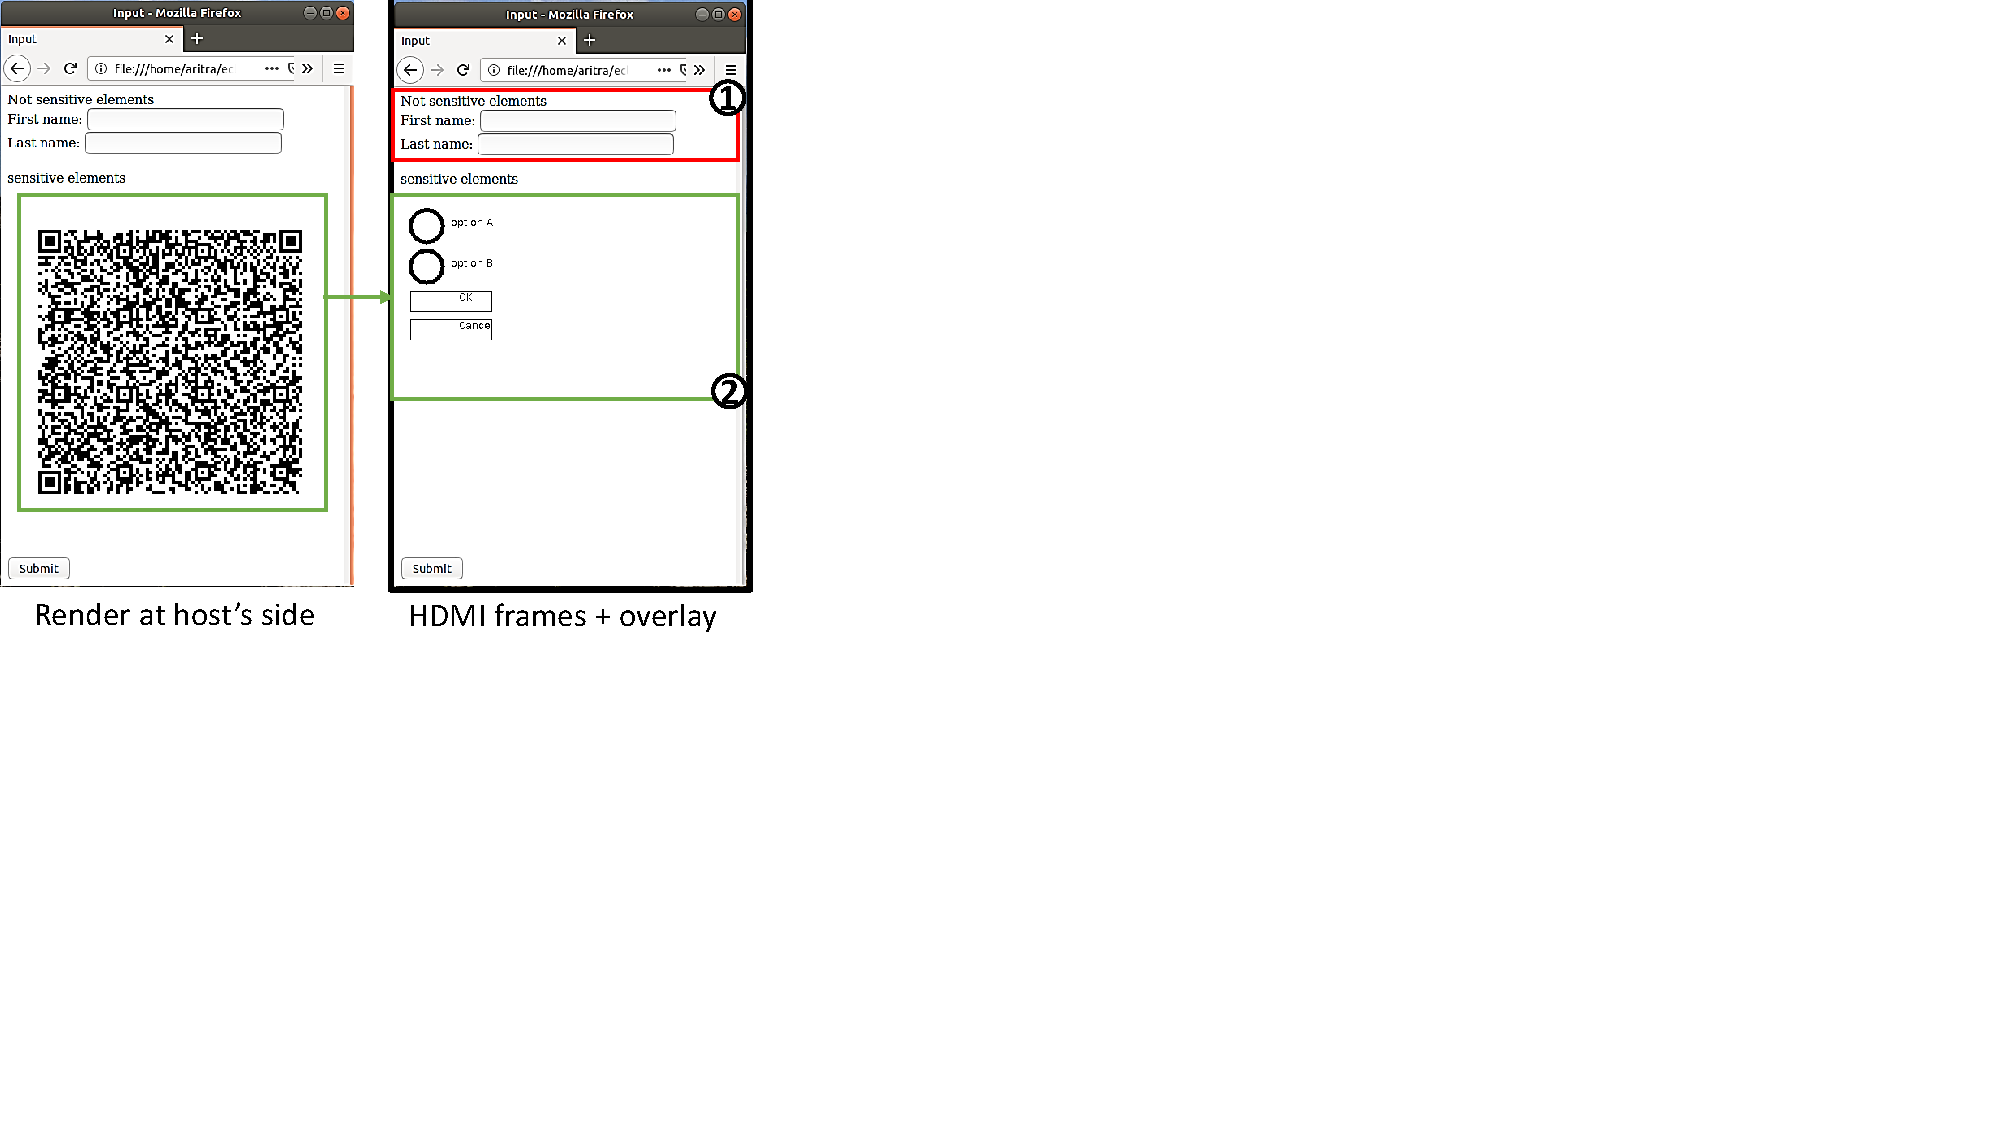
\includegraphics[trim={0 11cm 20cm 0}, clip, width=0.8\linewidth]{overlayScreenShot.pdf}
\caption{\textbf{\device generated UI overlay} that our solution use to hide the sensitive UI elements and inputs from the attacker-controlled host. Any input in the UI overlay is signed by the \device, hence the integrity of the user input is preserved.}
\label{fig:screenshot_1}
\centering
\end{figure}

\myparagraph{Components} \name assumes that IO devices (mouse, keyboard, and display) are connected to a trusted component called \device. This setup allows the trusted \device to receive raw inputs from the user and show overlays on display. The goal of \name is to keep the code running on the \device minimal and at the same time support a wide variety of applications. Thus, we avoid running any application, such as browsers, on the trusted component to keep the TCB very small.

\myparagraph{Key idea} The key idea of \name is to introduce \emph{root-of-trust} for the IO devices that provides trusted path to remote servers. This is achieved by the \device that provides proof for integrity and confidentiality for all user IO. Thus making the IO devices trustworthy to the users. The \device operates in two modes: passive and active. In the passive mode, the \device serves as a relaying device that forwards mouse and keyboard inputs to the host. Similarly, the \device relays the HDMI frames from the host to the display. Hence, the user experience is not affected when interacting with regular applications. On the active mode, \device has two functionalities: i) intercepts the inputs generated by the user, and ii) render overlays on the HDMI frame that is displayed on the screen. 
The first functionality guarantees that the user inputs arrive directly to a trusted component (\device); therefore, the compromised host cannot manipulate them. The second functionality allows the \device to show trusted information on the screen such as input elements, or data sent from the remote server.

During the initialization phase, the \device and the remote server share a key that is used to encrypt/sign the communication between each other. The remote server signs the sensitive elements that should be protected and delivers them to the untrusted host. The application running on the host encodes the sensitive elements into the HDMI frame. The \device captures the frames, decodes the sensitive elements, verifies their signatures, and then renders elements into an overlay. In this way, the device guarantees that the user is presented with the legitimate elements sent by the remote server and the user interaction with these elements is managed only by the device itself. Note that the device renders only the protected input elements, while other UI components of the application are rendered by the host. 
Therefore, user inputs (mouse events and keystrokes) addressed to the protected elements are intercepted by the \device and not forwarded to the untrusted host. Furthermore, the \device renders on runtime the user inputs into the overlay while the host is oblivious about them. From the user's perspective, the workflow of filling a form with protected elements remains the same as filling forms of existing applications.

\myparagraph{Our realization of \name} \name in principle can work with generic host and application. In our prototype of \name, we implement a version of \name that works with web applications running on the browser. Our implementation of \name is realized by a low-TCB auxiliary device that acts as a hub for all IO devices. This also eliminates any need for additional software that acts as a communication channel between the \device and the host. The server and the \device communicate with QR codes. As the host renders the QR code on the screen, the \device decodes the QR code from the HDMI channel. One such example is illustrated in Figure~\ref{fig:screenshot_1} where the server sends a QR code that encodes a sensitive input form. The \device first intercepts the HDMI frames, then decodes the QR code in that frame and overlay the decoded form on the display that can be seen only by the user. Our realization of \name achieves the goals that we mentioned in Section~\ref{sec:problemStatement:goals}. \name supports generic IO devices and provides IO integrity and confidentiality (\textbf{goal 1}).The \device is implemented using a low-TCB embedded device that minimizes trust assumption (goal 2) and the \device is plug-and-play and requires minimum user habituation (goal 3). 


\subsection{Challenges}

%Modern user interfaces are extremely complex to analyze, and such allows many possible ways to provide input. This makes the protection of IO integrity, and privacy is a particularly challenging task. For example, given a command from the user, it is necessary to understand the user intention that corresponds to the mouse movements. Given the screen space, there exist a multitude of ways for the user to move a mouse a place on a specific UI element that fires a command to the remote end system. To provide an end-to-end protection to this entire activity one needs to 1) precisely track the cursor position, 2) correspond the cursor location to the given movement data from the mouse, 3) understand the semantics of the UI element the fires the command, and 4) generate an efficient and comprehensive proof that the server can use to understand the user's real intention.

Modern user interfaces (UIs) are diverse and hard to generalize, resulting in many possible ways to provide input and receiving output.  This makes the protection of IO integrity, and confidentiality is a particularly challenging task. For example, given a mouse movement and clicking on a button from the user, it is necessary to understand the user intention that corresponds to the mouse movements. One naive solution would be to record a continuous screen capture of display and send it to the server. As the screen capture captures all the information displayed on the screen, later review should uncover if the attacker attempts to manipulate the UI or the IO data. Even though this naive solution provides strong security guarantee, it is impractical. So, the first challenge arises to build a secure system that is feasible and can be generalized with all the IO devices.   

The second challenge arises while ensuring IO confidentiality. For mouse input, hiding the mouse movement while keeping all the regular functionality intact is a challenging task as we do not consider large TCB-based solution such as a trusted hypervisor.


Apart from these functional challenges for implementation, there exist multiple attack vectors that we want to provide protection. An attacker that controls the entire host can lunch complex UI-based attacks. Such includes spawning multiple mouse pointer to trick the user into following the wrong mouse pointer, changing the layout of the UI elements to trick the user into providing sensitive data, tricking the user into moving the mouse to the wrong location and click there, manipulate input data, etc.





\iffalse
\subsection{Approach}

The main objective of our approach is to provide a secure channel between the user IO devices and the remote server that provides integrity and privacy of the IO data. Our solution uses the \device as the IO \emph{root-of-trust}. The \device that can be either integrated into the graphics card or can be used as a stand-alone auxiliary device (as we did in our implementation). The \device taps into the HDMI channel extract frames and determine the current context of the user's action. The \device also can overlay bitmaps into the HDMI channel. By doing this, the \device provides security properties to the IO devices that are illustrated in Figure~\ref{fig:screenPartition}. Using such capability, our system provides the following security properties: \emph{\pop}, \emph{\poui}, \emph{\poa}, and integrity and privacy of the IO.

\myparagraph{\Pop} All the keyboard and mouse input from the user is intercepted by the \device. The \device uses the raw mouse data from the user, and on the screen, it detects the corresponding position of the mouse pointer. The \device captures a trace of the mouse pointer position and the click data. Using the mouse trace data, the \device computes a \emph{\pop}. The \pop serves as an indirect measure for the input integrity as the \device confirms the remote server that if the user drags/clicks the mouse in a way that results in an input to the remote server. The \device also overlays a mouse-pointer image on the host's cursor. The overlaid mouse pointer is conspicuous to the user and uses as a safeguard if the host generates multiple pointers. Additionally, the \device employs secure attention sequence (SAS) mechanism that dims all of the display except the overlaid UI and the mouse pointer for user attention.

\myparagraph{\poa} \Poa guarantees that a specific command that is sent to the server is indeed issued legitimately by the user. Any action on the overlaid region of the screen is recorded and signed by the \device.  Direct inputs such as clicking a button or a text data in a text box are signed by the \device and sent to the remote server. These signed input data serves as the second-factor fort the input integrity. The server receives and matches the \emph{applications-level} payload from the browser and the \emph{signed second factor} from the \device. 

\myparagraph{\Poui} All the UI elements that are displayed on the overlaid area is rendered by the \device and signed by the remote server. \Poui ensures that a UI that is seen by the user is legitimately generated by the remote server and reconstructed faithfully by the \device. The JavaScript snippet that is served by the remote server transforms the security-critical UI of the webpage to a QR-code encoded specification. The \device detects the QR code by intercepting the HDMI frame between the host and the display \device. The specification is signed that provides the integrity and the authenticity of both the output data and the UI objects on the webpage. 

\myparagraph{IO integrity and privacy} As the \device also sits on the HDMI channel between the host and display \device, it can overlay objects on the HDMI stream and thus achieves display integrity and privacy. All the objects that are overlaid by the \device can be seen only by the user, and the host is oblivious to the IO.


\fi
\begin{figure*}[t]
\centering
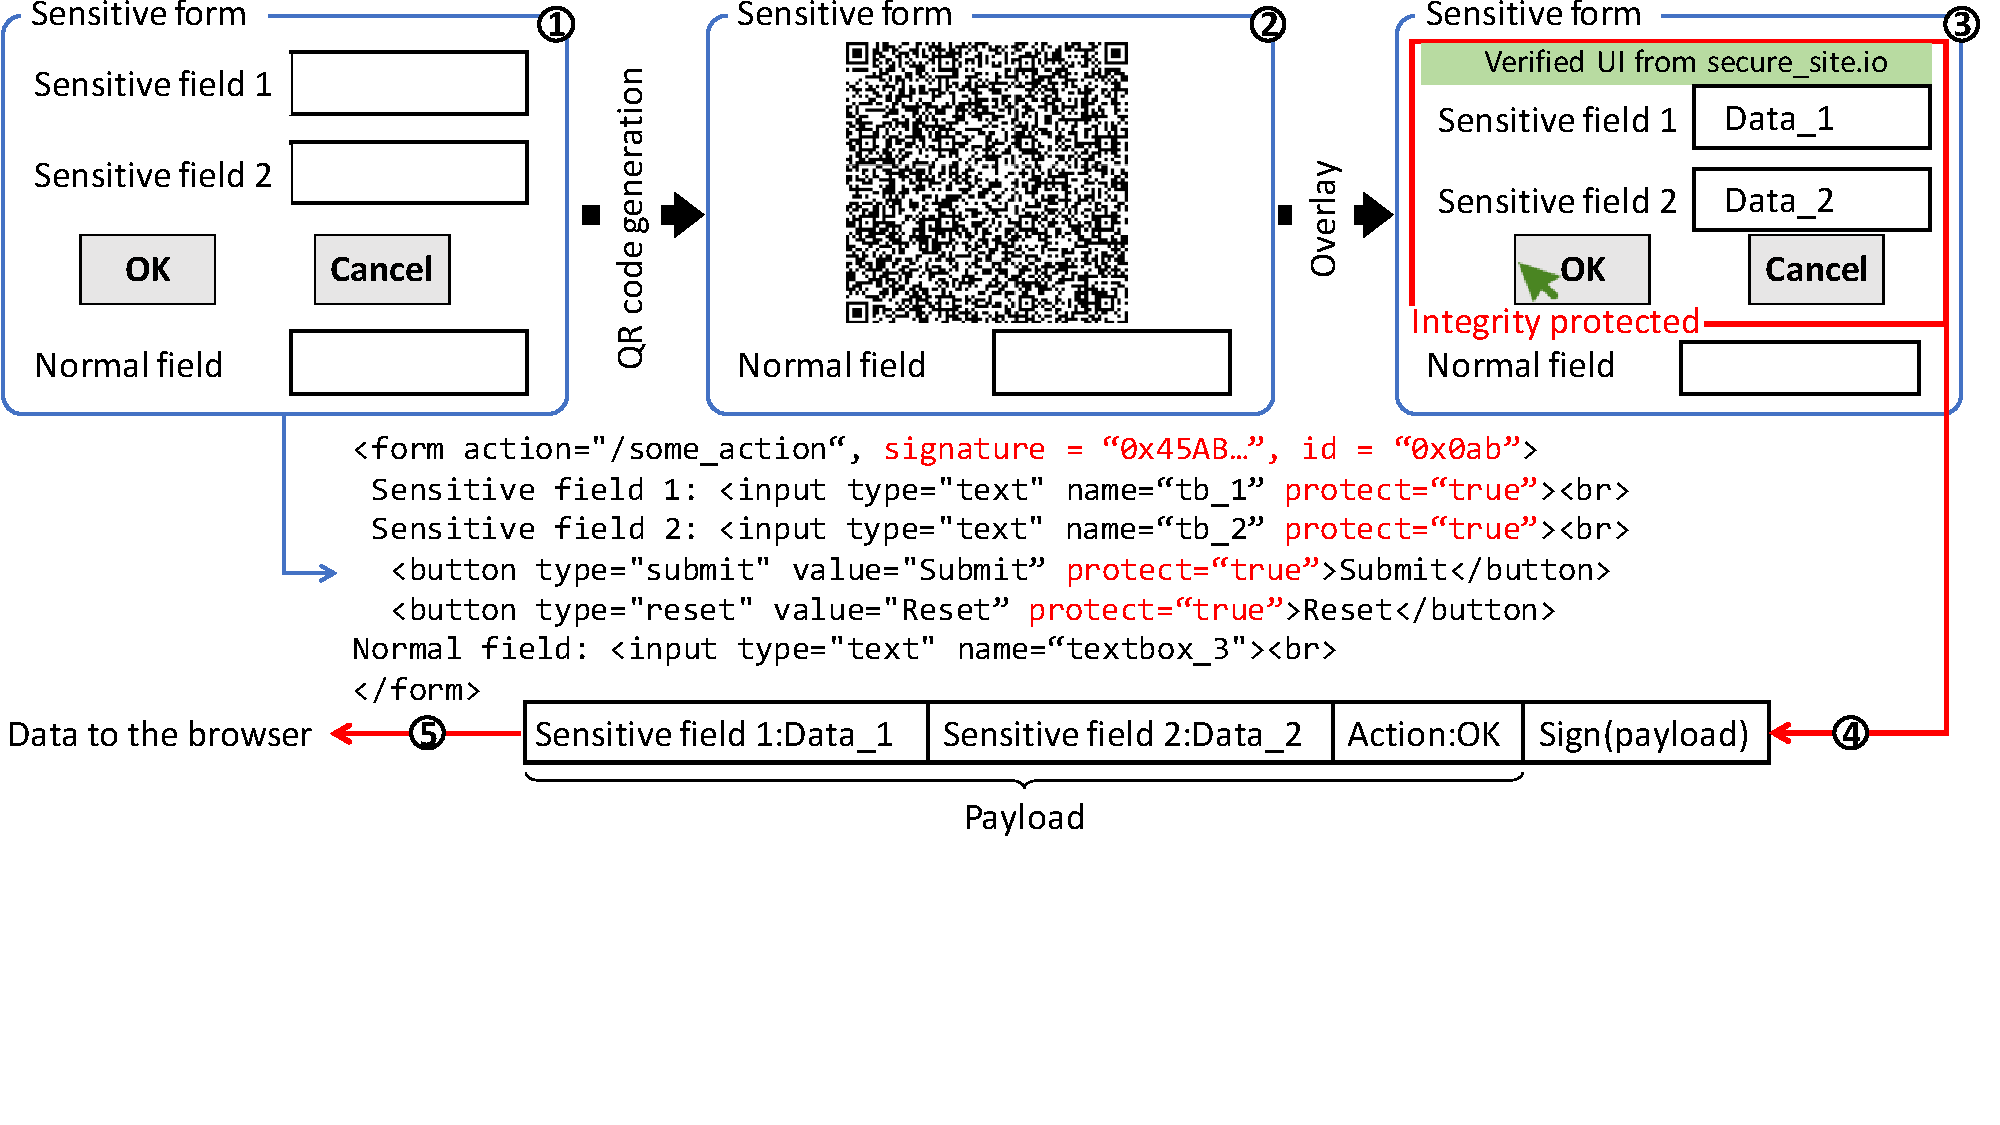
\includegraphics[trim={0 4.8cm 0 0}, clip, width=0.8\linewidth]{formTransform.pdf}
\caption{\textbf{Transformation of UI elements: HTML $\rightarrow$ encoded specification $\rightarrow$ \device generated UI overlay.} \one The actual webpage and the corresponding \html source shows the UI elements that requires integrity protection. \two These UI elements are transformed into an encoded UI specification (our \name prototype uses QR code that encodes a UI specification, e.g., Specification~\ref{snippet:UISpecification}) by the \name JS. The QR code. \three AThe QR code decoded and overlaid on the HDMI stream by the \device. \four Upon the user's action on the overlaid UI elements, the device signs all the input data. \five The \device sends these signed input data them to the remote server. Note that the intermediate QR code transformation (\two) is not visible by the user as it is decoded instantaneously by the device.}
\spacesave
\label{fig:transformation}
\end{figure*}

\section{\name for IO Integrity}
\label{sec:systemDesign}



\lstset{language=JSON, frame=tb, caption=\small{\textbf{Protected UI specification language.} The UI specification shows the JSON formatted UI specification that is generated from the \html source provided in the UI illustrated in Figure~\ref{fig:transformation}.}, label=snippet:UISpecification, firstnumber =1}

\begin{figure}[t]
\scriptsize
\begin{lstlisting}[mathescape=true]
{ "formId": "form1", "formName": "form1",
  "domain": "secure_site.io",
  "size": "400*400", "SAS": "5:LB",
  "ui": [{"id":"textbox_1", "type":"textbox", 
      "label":"Sensitive field 1",
    "text":"secret data 1",
    "RE":(A-Z)*.(A-Z)*},
    {"id":"textbox_2", "type":"textbox",
    "label":"Sensitive field2 ",
    "text":"secret data 2"},
    {"id":"b1", "type":"button",
    "label":"OK", "trigger":"true"},    
    {"id":"b2", "type":"button",
    "label":"Cancel", "trigger":"false"}],
  "signature": "0x45AB...", "id": "0x0ab.."}
\end{lstlisting}
\spacesave
\end{figure}

%In this section, we provide the technical details of \name for the integrity protection of IO devices. 
In this section, we provide the technical details of \name that guarantees the integrity of IO operations.


\subsection{\device Overlay of UI Elements}
\label{sec:systemDesign:transformation}

As we explained in the previous sections, both output and input integrity are necessary to be protected to achieve any of them. \name ensures output integrity by isolating a part of the display that cannot be observed or modified by the untrusted host. \device intercepts the HDMI frame from the host and injects a render of the sensitive UI on the screen. The overlay provides output integrity because it restrains the attacker from drawing on top of it to trick the user into providing incorrect inputs. 

To minimize the TCB, the \device does not run a browser, i.e., it can not interpret or render HTML, \js, etc. Instead, the \device comes with a small interpreter routine that is similar to render engines of browsers in functionality, but drastically smaller in size because it only renders a limited number of HTML5 UI elements according to their position, dimension, and label. The interpreter routine reads a given specification and renders the respective UI. The specification is a simple \emph{JSON} file that defines how the content of the overlay should be rendered, e.g., number of elements, order, types, and labels. \red{One strawman solution could be sending UI bitmap from the server to the \device and the \device could send back the mouse click and the corresponding location. \device could download these pre-generated form bitmaps from the server, and such solution would handle static forms, but not for dynamic forms. Downloading all possible form bitmaps would be prohibitively expensive.}

The process of rendering the overlay on the screen has two phases: (i) convert the existing sensitive form to specification, and (ii) specification to overlay.

\myparagraph{(i) Secure form $\rightarrow$ Specification} The W3C UI security policy~\cite{w3c_spec} recommends developers to annotate the security-critical UI elements of a page to protect them against malicious JS running on the browser. We use a similar technique by asking developers to manually annotate the sensitive elements in the HTML code (as \texttt{protect=``true''} attribute). Then For every request, the \name server-side component parses the HTML source, adds a random identifier (\texttt{id}) to the \texttt{form} element, signs it, add the \texttt{signature} to the \texttt{form} and then delivers it to the user's browser. The \texttt{id} serves as session identification to prevent the attacker from re-submitting an old input data from the user. On the client side, \name JS parses the tagged HTML source and produces a specification that can be interpreted by the \device.  An example of a specification is presented in~Specification~\ref{snippet:UISpecification}. In our implementation, the \name JS encodes the specification in a QR code. \red{We choose QR codes as it is one of the many robust was to encode data on a visual channel such as HDMI stream.} Figure~\ref{fig:transformation} shows the transformation between the step \one and \two. The step \two is processed by \device in the next phase and is not visible to the user.


%We further optimize this process that does not require to add the UI specifications into the HTML sources. The developers include small JavaScript code: \name JS to their sources. \name JS has the same functionally as the server side code that parses the HTML code and outputs the specification. Note the specification generation process is deterministic, hence, given identical HTML sources, both server and the \name \js generate identical UI specifications. Note that \name JS runs on the browser and is not trusted in our system model. We illustrate the method of UI transformation in Figure~\ref{fig:transformation}. 


\myparagraph{(ii) Specification $\rightarrow$ Overlay} \device performs the next phase, which starts with the detection of the encoded specification (QR-code) in the HDMI frames. Then the \device validates the signature, renders the overlay according to the specifications and presents it to the user.  The \device overlay is depicted in \three in Figure~\ref{fig:transformation}, which is the final UI shown to the user. Note that the user does not see the QR code as it gets decoded and overlaid by the \device on the fly.

\device uses the specification to determine the particular UI element that the user interacts with. When the user clicks on a text field, \device allows the user to type input to it. UI elements in the overlay take inputs only from input devices (mouse and keyboard). Therefore a malicious host cannot inject or modify any input of the user.

\subsection{Focusing User Attention}
\label{sec:systemDesign:userAttention}

In the previous section, we explain how \name provides output integrity for the overlay generated by the \device. However, the attacker can show fake information to the user on the untrusted part of the display space that may potentially influence her inputs. An advanced adversary could craft malicious directions and present to the user as part of the overlay.

To mitigate these attacks, we employ techniques that are proposed against similar threats in the context of browser-based security. The goal of these techniques is to focus user attention to the sensitive UI elements she is interacting with. Huang et al.~\cite{huang2012clickjacking} proposes two main techniques that are shown to be effective and can easily be adopted by the \device.  The first technique is called Lightbox, and it dims out non-overlaid part of the screen, which is generated by the untrusted host. The second technique consists of freezing display frames from the host when the user enters into the overlaid UI. This way, a malicious host cannot grab the user's attention by showing an animation or exploiting other tricks.
Lightbox offers more security guarantees because it blocks the untrusted screen completely, but is more intrusive to the user. While freezing is less intrusive but does not remove potential malicious information from the screen.
Lightbox mitigates the attacks presented above. The paper shows that the lightbox and freezing are effective in $98\%$ and $97\%$ of the time (baseline: $69\%$ effectiveness when no protection is provided) respectively, making them suitable candidates for \name. For more details of the user study, refer to Table 2 in~\cite{huang2012clickjacking}. We assume that similar result should be expected in \name due to the similarity of the application space (web applications). \device uses Lightbox as the default technique, but depending on the specific form, the developers can select the appropriate technique.

\red{Note that during the time the focusing mechanism (such as the LightBox) is active, the user can still interact with the UI elements outside the secure UI elements as the \device does not control those. Browser back button is also accessible by the user but it does not influence the state of the overlaid UI as long as the back button does not remove/change the QR code on the web page.}

\myparagraph{\bfseries Automated activation} The technique to focus user attention (dimming out or freezing the non-overlaid part of the screen) is triggered automatically in specific situations: The user moves the mouse pointer over the overlaid UI, or the user starts typing into a sensitive UI element. 
%e.g., when the user moves her mouse pointer over the overlaid UI, or start moving the mouse after a brief pause (like 5 seconds). 
The advantage of the automated trigger is that the user does not need to remember to activate the mechanism. Hence the system is resilient from user habituation and does not require the user to actively monitor security indicators or perform specific actions. Note that the automated activation provides security to user IO data \emph{only} when integrity of the data is considered.

\subsection{Continuous Tracking of Mouse Pointer in the HDMI Frame}
\label{sec:systemDesign:analysis}


\begin{figure}[t]
\centering
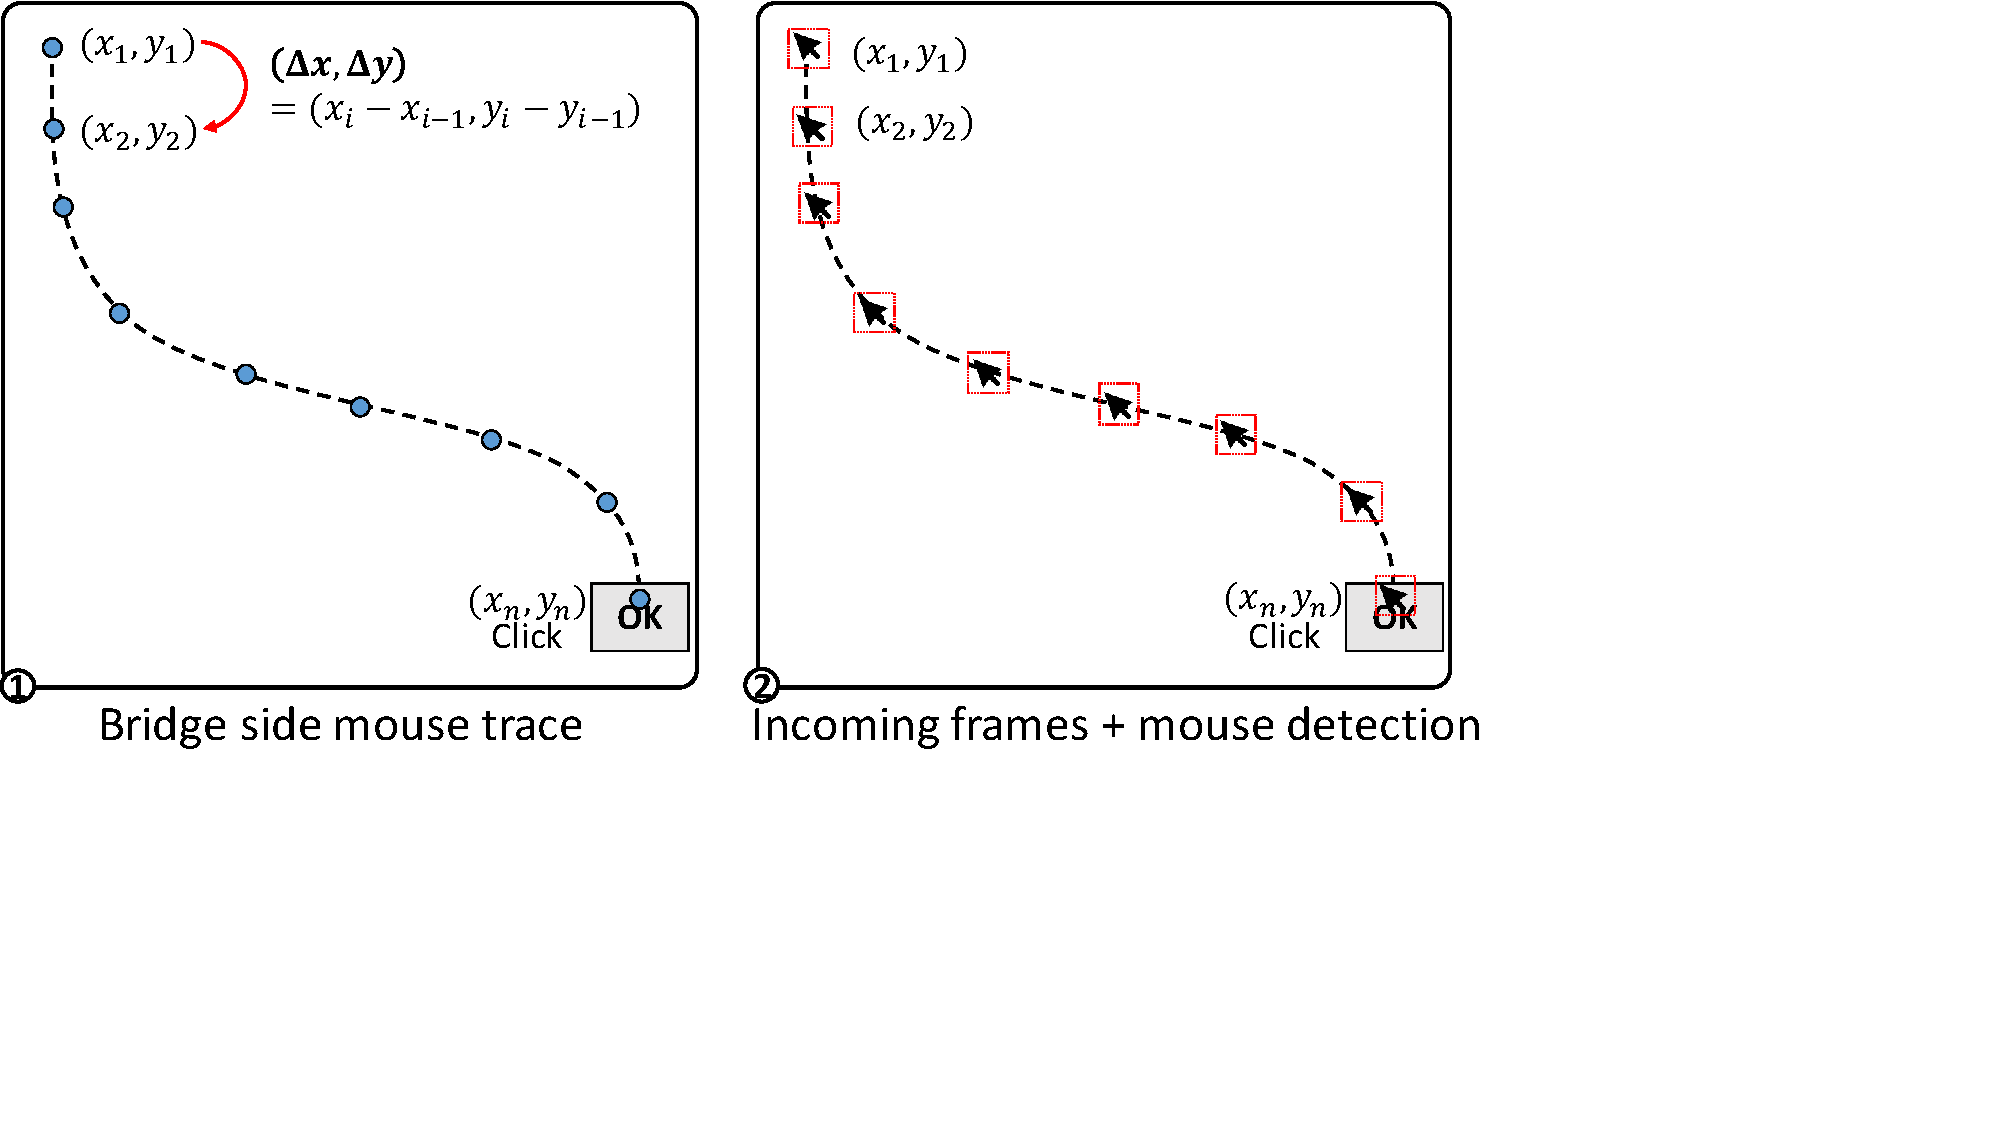
\includegraphics[trim={0 5.8cm 8cm 0}, clip, width=\linewidth]{mouseAnalysis.pdf}
\caption{\textbf{Pointer tracking.} \one The \device captures the raw mouse events ($\Delta x, \Delta y$) from the mouse that is attached to the \device. \two The \device captures the frames from the HDMI channel and checks into the designated pixel position $(x_i + \Delta x, y_i + \Delta y)$ if there exists a pointer. $t_1, t_2,\ldots t_n$ are the time instances when the \device receives the mouse data. $f_1, f_2,\ldots f_n$ are the corresponding HDMI frames that the \device intercepts.}
\spacesave
\label{fig:mouseAnalysis}
\centering
\end{figure}


The triggering of the focusing mechanism poses a challenging task to \name because the \device does not know the exact position of the mouse pointer. We cannot rely on the compromised host to communicate the pointer position reliably to \device. Furthermore, the host's pointer is not visible when the user interacts with the overlay rendered by the \device as the \device always draws on top of the HDMI frames of the host. 
%To address this issue, \name continuously tracks the host's mouse pointer from the HDMI frame (using shape detection) as it has access to both the HDMI channel and the raw mouse data.

\device could employ image analysis over the frame received from the host to learn the pointer position. However, we avoid this method because image analysis is time-consuming and vulnerable to adversarial images. In our approach, the \device intercepts mouse events and HDMI frames, so it can track the pointer based on mouse data and correlate it with the actual position in the HDMI frame (using shape detection in a small area). Then, the \device overlays a mouse pointer that is prominent and easy to follow by the user. 

A malicious host can still show a fake pointer to trick the user into following it, but when the focusing mechanism is active (the user interacting with sensitive elements), only the pointer overlaid by \device is visible. This way, the pointer tracking and the pointer overlay address three major challenges: i) both the \device and the user have the same sense of the pointer position, ii) \device knows precisely when to trigger the focusing mechanism, and iii) the user can interact with the overlaid UI seamlessly. 


\subsubsection{\bfseries Calibration}\label{sec:systemDesign:analysis:calibration} When the user connects the \device for the first time after booting up, the \device performs an automated calibration to find the pointer. The \device simulates the mouse and pushes the pointer to the top-right corner of the screen. Then the \device searches the pointer at this position in the HDMI frames
%If the \device is successful into finding the mouse pointer, 
and starts tracking the pointer afterward. Note, that at any point, if the \device loses track of the mouse pointer, the \emph{calibration} process is repeated the first moment the user visits a website that employs \name.
%user can recalibrate it by reinitializing the \device.

\subsubsection{\bfseries Pointer detection} The \device ensures pointer integrity by tracking the mouse movements using the raw data from the mouse and the HDMI frame.  Figure~\ref{fig:mouseAnalysis} illustrates the high-level idea: 

\begin{mylist}
\item[]\one Shows raw mouse data that notify the displacement events $(\Delta x, \Delta y)$ over $x$ and $y$ axis which are fired over time series $t_1,\ldots, t_n$. Note that the initial pointer position is known to the \device from calibration phase where $(x_0, y_0) = (0, 0)$.  
\item[]\two Shows the HDMI frames $f_1,\ldots f_n$ where the \device expects the mouse pointer to be found. For efficiency, the \device only scans a small portion of the HDMI frames ($200 \times 200$ square pixels) that is enough to cover a mouse pointer. Since the operating system can treat mouse movements slightly different according to their algorithm, this step serves to adjust the position difference.
%\device checks if there exists a mouse inside this square or not. \red{In case there exists a mouse cursor, the \device allows further user interactions; otherwise, it stops all the communications and shows an error on display.}
\end{mylist}


\subsubsection{\bfseries Overlay of the mouse pointer} The \device draws a mouse pointer overlay on top of the actual mouse pointer. The host mouse pointer is neither visible on top of the overlay nor it can interact with the \device's overlay. The overlaid mouse pointer is visible on top of the overlay, and it offers the same user experience as the host-rendered mouse pointer.


\subsubsection{\bfseries Coping with the disappearing pointer} Many OS offer a feature where the mouse pointer disappears from the screen when the user types in a text editor/browser. When the user moves her mouse, the cursor appears again at the same position where it disappeared in the first place. From the \device's perspective, it is hard to distinguish between this case and the attacker deliberately removing the mouse pointer from the screen. To handle this case, the \device listens to all the keyboard inputs -- the keyboard is also connected to the \device. Therefore, when the \device gets a keystroke event, it expects the cursor to disappear from the screen. Then, \device continues tracking the pointer from the moment that the mouse sends events  - this way, the \device ensures the consistency of the pointer position.  


\subsubsection{\bfseries Handling different mouse cursors} The \device is preloaded with template images of the mouse pointer for detection. For our \name prototype implementation, we use the default cursors provided by the Ubuntu OS. This allows the \device to identify the cursor when it changes on the screen, e.g., from pointer to a hand when the user hovers the pointer over a link on the browser. 

 
\subsubsection{\bfseries Handling mouse acceleration} The \device uses the default mouse acceleration parameters of \texttt{libinput} to cope with the pointer acceleration. As the \device emulates itself as a keyboard, at the time of initialization, the \device sends a command to the host to set the default acceleration. In case, the host changes the mouse acceleration; the \device will fail to detect the mouse in the HDMI stream. We consider this case as a denial of service.

\subsubsection{\bfseries Entering/exiting secure mode with keyboard} \red{In our implementation of \name, entering and exiting the secure mode could only be done by the mouse pointer. But similar could be done by the keyboard also. User could use the \texttt{TAB} button that selects the QR code on the browser. In the \name JS, we can define properties that triggers some changes (by changing the selection parameter) into the QR specification that signals the \device to enter/exit the secure UI.}

\begin{figure}[t]
\centering
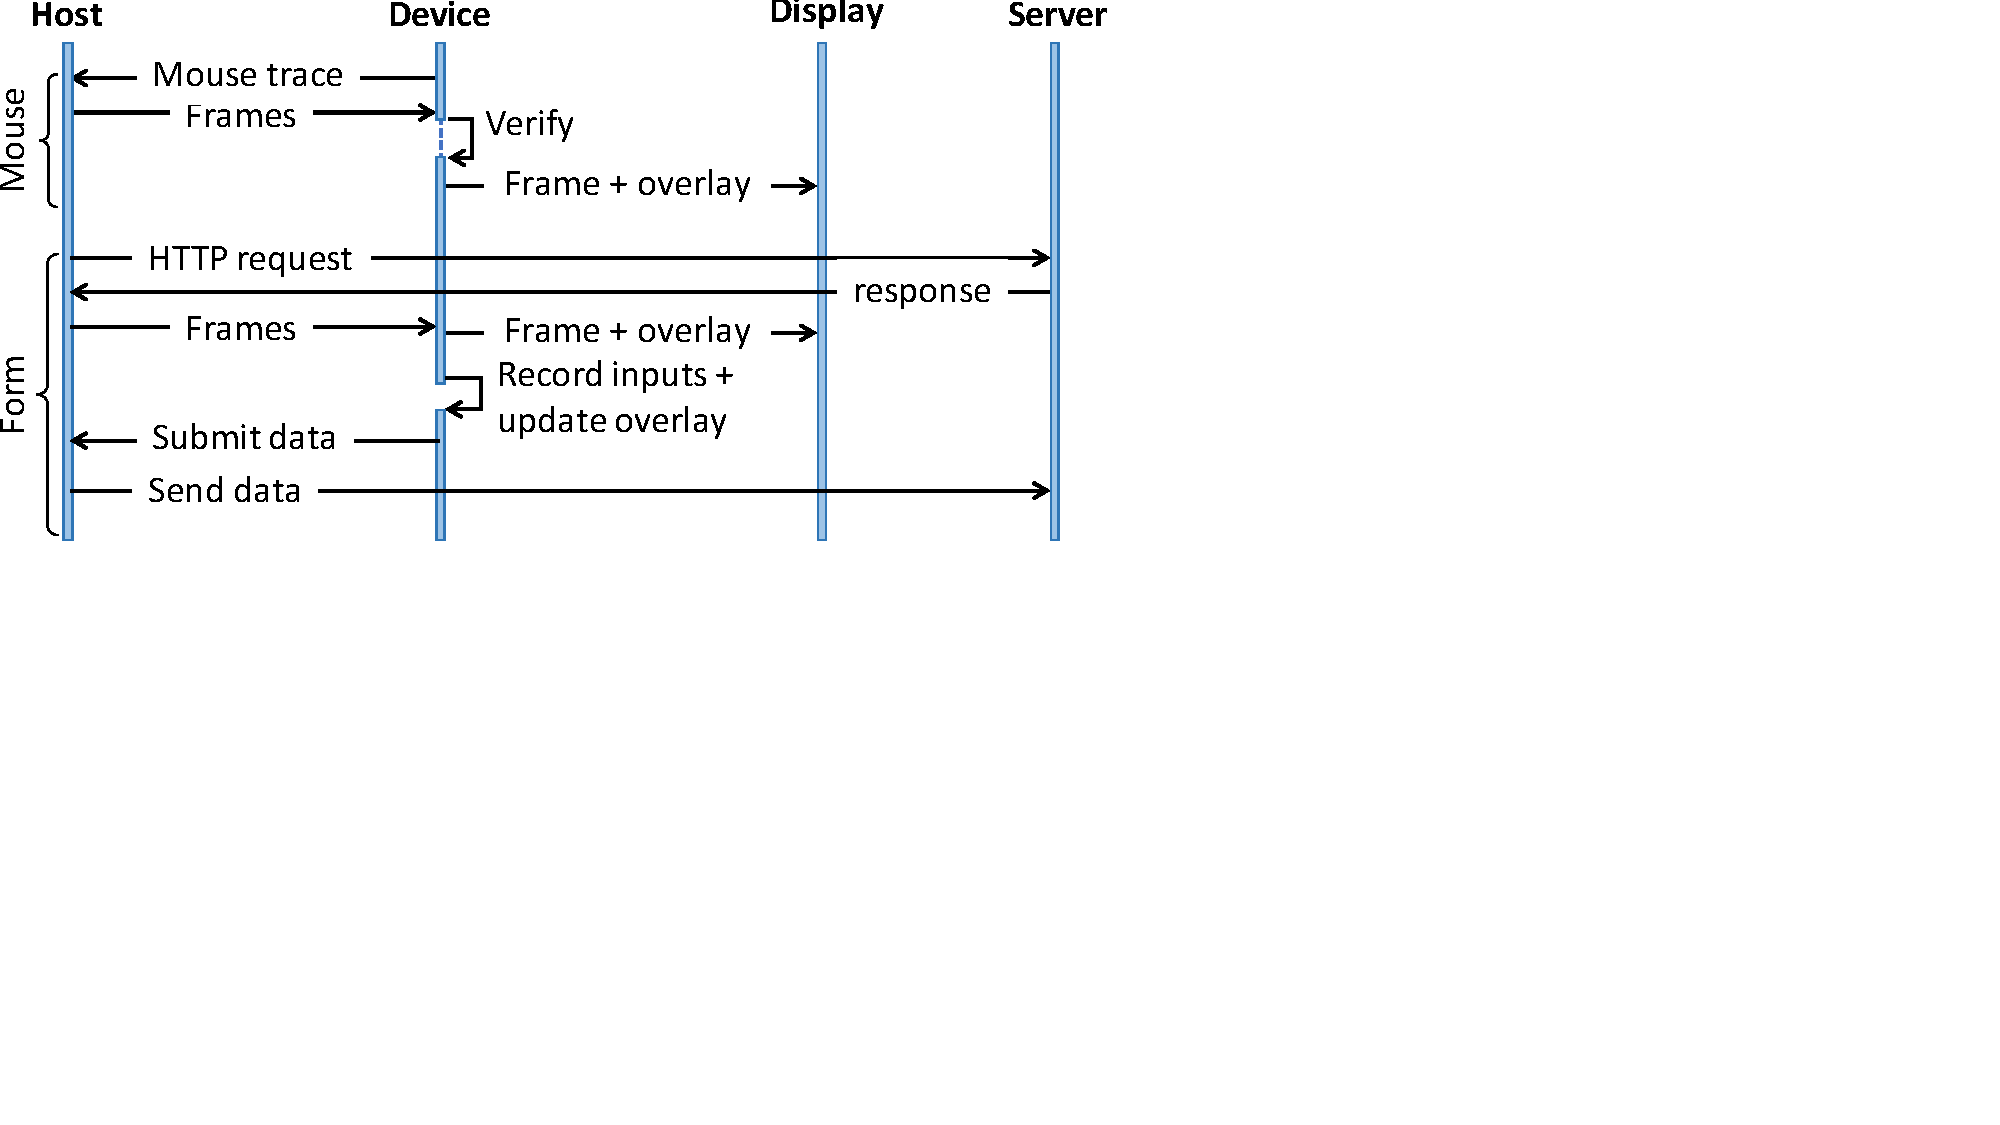
\includegraphics[trim={0 9.5cm 15cm 0}, clip, width=0.85\linewidth]{SequencDiagram.pdf}
\caption{\textbf{Flow of the \name main protocol.} The figure shows the sequence of events for two example scenarios: mouse movement and filling up a web-form.}
\spacesave
\label{fig:sequence}
\centering
\end{figure}


\subsection{Protected User Interaction}
\label{sec:systemDesign:commit}

When the user finishes providing her input via input devices (mouse and keyboard), the \device sends these values (with signature to ensure integrity) to the remote server. Sending these signed input values to the server requires an upstream channel from the \device to the server. 

\myparagraph{Upstream channel}\label{sec:systemDesign:commit:upload} 
The data from the \device to the remote server is transmitted using the \name JavaScript snippet as a helper. 
%The \name JavaScript snippet uses a hidden text field to accept data coming from the \device. 
The \device emulates itself as a composite human interface device (HID) when it is connected to the host. The \device emulates keystrokes that transmit encoded data to the \name JavaScript snippet, which then forwards them to the remote server.

\myparagraph{Sending input data} Figure~\ref{fig:sequence} depicts the user interactions in a sequence diagram. The user input transmission procedure is illustrated in Figure~\ref{fig:transformation}. This has two phases: \emph{record} and \emph{transmit} as described in the following:

\begin{mylist}
\item \textbf{Record.} After the UI elements are correctly overlaid on the screen, the users can interact with these UI elements. The user interaction with the overlaid UI element is no different than a standard UI. The UI specification encodes the behavior of all generated UI elements, making the \device aware of the semantics of the UI objects. E.g., when a user selects a text box and types on with her keyboard, the \device intercepts all keystrokes and renders the characters on the overlay.
When user enters input data in the rendered overlay UI elements (such as textbox, button, slider, radio button, etc.), the \device records that in a (key, value) pair where the key is the identifier of the UI element (\texttt{id} in Specification~\ref{snippet:UISpecification}) and the value is the user provided value. The \texttt{type} of the UI elements determines what information to record. For example, the \device records all keystrokes when a textbox is selected, the value corresponding to the position of the slider is recorded when the user interacts with a slider, etc. One example of the recording of the input data corresponding to the UI illustrated in Figure~\ref{fig:transformation} and Specification~\ref{snippet:UISpecification} is: 
\begin{align*}
Record = & (tb\_1, Data\_1);(tb\_2,Data\_2)
\end{align*}

\item \textbf{Transmit.} In the transmit phase, the \device waits for the user to select a UI element which has a \texttt{trigger} capability, e.g., a submit button on a web-form. A trigger element can change the state of the overlaid form, e.g., submit the data of the form to the remote server or reset it. More details are provided in the implementation of \name in Section~\ref{sec:prototype:impl:qr}. When the user clicks the \texttt{OK} button, the device signs $Record$ with its embedded private key. One such signed packet is also illustrated in Figure~\ref{fig:transformation}. The \device sends the signed packet to the remote server using the upstream channel.
\end{mylist} 

%\subsubsection{\bfseries Server-side verification} \label{sec:systemDesign:commit:verification}
Upon receiving the signed input data from the \device, the remote accepts the input if the signature verification is successful. Note, if an input field is annotated as \texttt{protect=``true''}, the server does not accept any input without the \device signature. This prevents the attacker-controlled host to submit data. 

\myparagraph{Changing browser tabs or browsers}
The \device supports multiple browsing tabs across multiple browsers. The UI specification contains \texttt{formId} and \texttt{domain} that works as the unique identifier for a specific form served from a specific web server. The \device can maintain multiple parallel TLS connection to web servers. Depending on the observed \texttt{formId} and \texttt{domain} (refer to Specification~\ref{snippet:UISpecification}), the device retrieves the data that is entered by the user. This way even if the user switches tabs, the \device can still allow editing the forms across tabs.

\myparagraph{Input validation} Input validation, i.e., checking the input against a recommended input policy (e.g., regular expression) is one of the most widely used JavaScript functionalities and it is a critical part of input integrity. The remote server sends the regular expression in the UI specification (\texttt{RE} in Specification~\ref{snippet:UISpecification}) that the \device uses to validate the user input.

%\myparagraph{Sequence of Events} In the previous Sections, we explain the basic components of \name. Here we summarize the overall flow of the system. The sequence diagram of \name is illustrated in Figure~\ref{fig:sequence} that shows snapshots of two example sequences: mouse movement and filling up a web-form.

\myparagraph{Fallback for legacy clients} \name is backward-compatible with the clients who do not use the \device. This is achieved by the remote server by showing a QR code briefly on the screen when the user visits the \name-enabled webpage. The \device intercepted the QR code and sends a signal to the server about its presence. In the absence of the \device, the remote server does not send the \name JS to the host that acts as a communication channel between the \device and the remote server. Note, that the fallback mechanism is application-specific and the service provider could decide if the fallback is detrimental to security.
\iffalse
\begin{figure}[h]
\centering
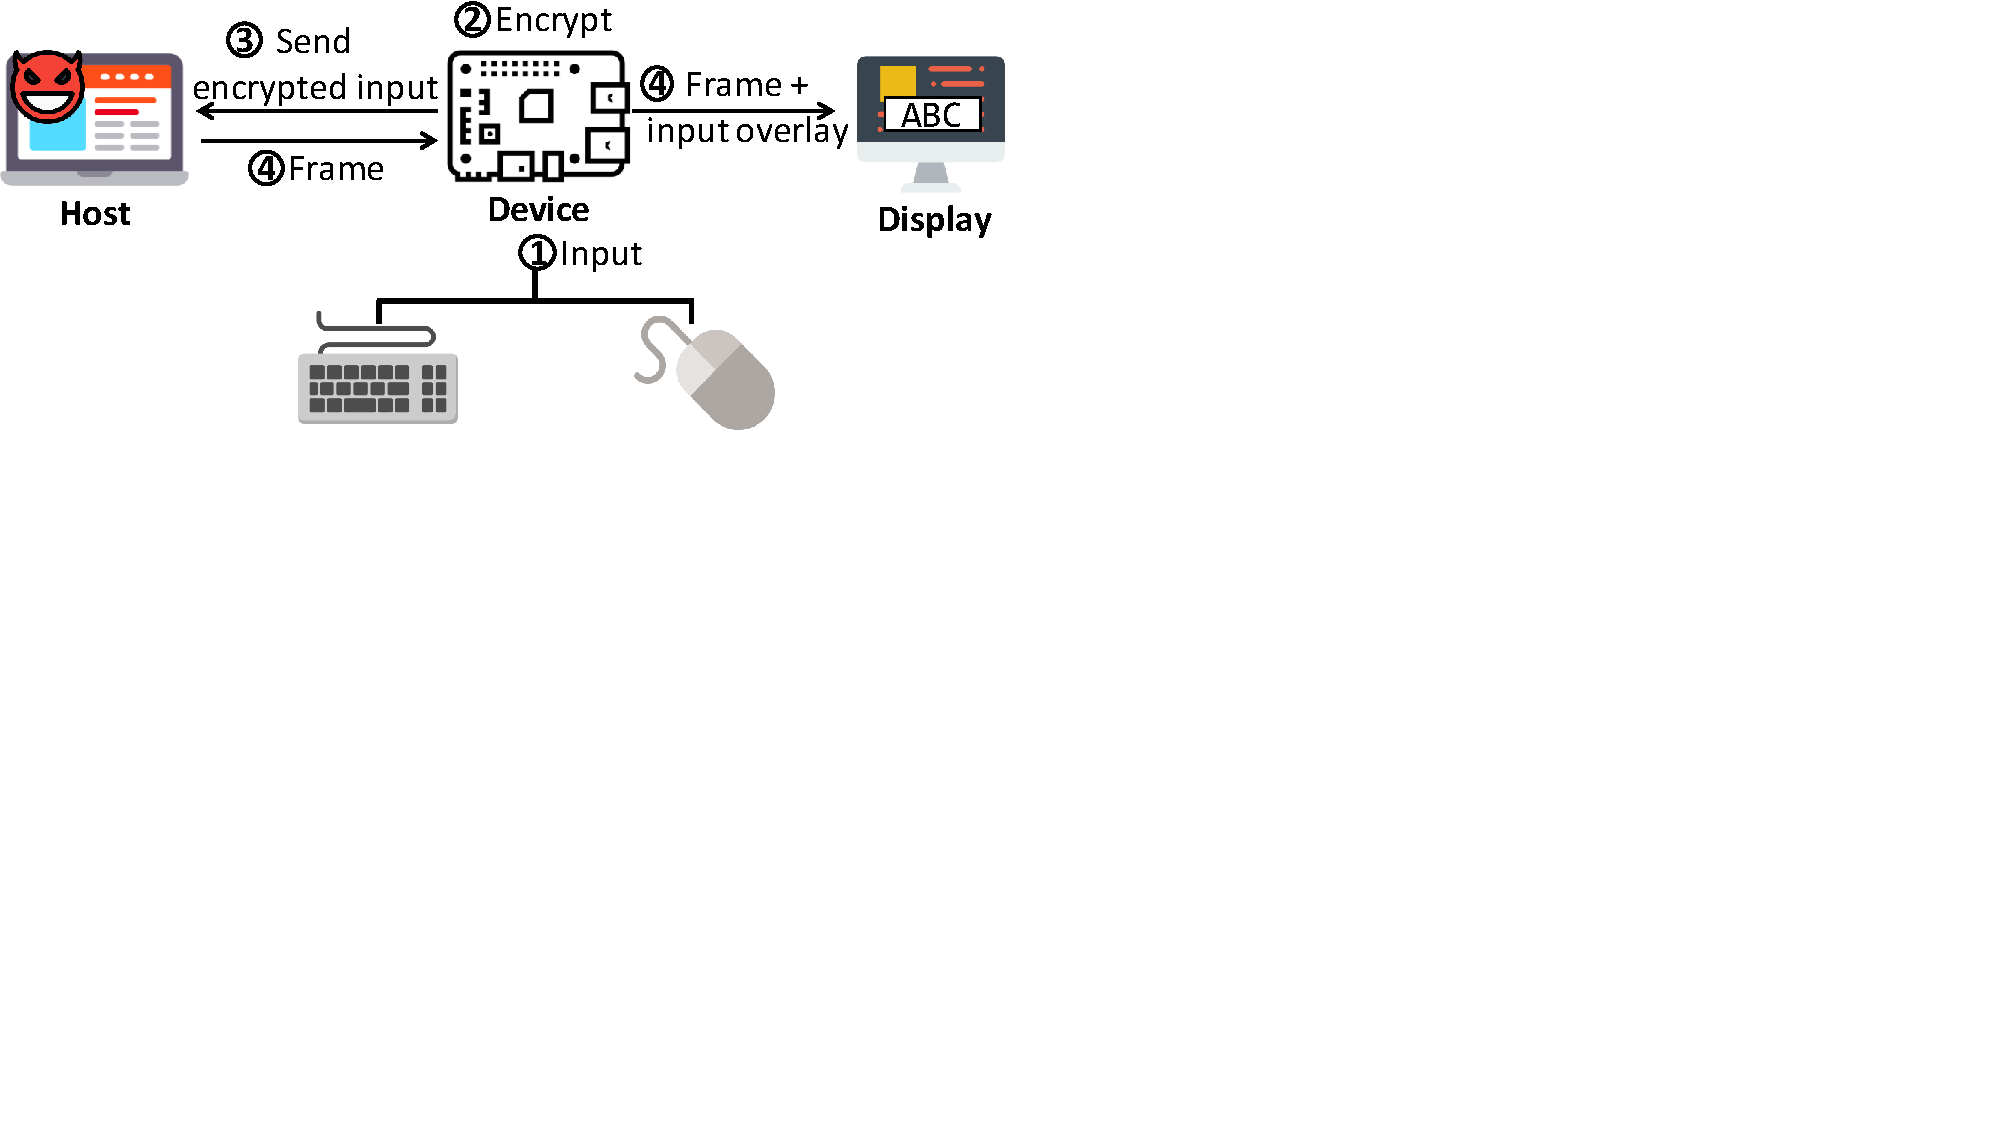
\includegraphics[trim={0 11cm 16.5cm 0}, clip, width=\linewidth]{inputPrivacy.pdf}
\caption{Input Confidentiality}
\label{fig:inputPrivacy}
\centering
\end{figure}
\fi



\section{\name IO Confidentiality}
\label{sec:confidentiality}


In the previous sections, we describe how the \name \js and the \device together ensure the integrity of the IO. We now augment the design of \name achieve IO confidentiality alongside of the IO integrity. One of the major components for achieving IO confidentiality is to establish a secure channel (i.e., a \tls channel) between the remote server and the \device. \tls ensures that all the IO data from/to the user is hidden from the untrusted host.  

\subsection{Establishing \tls}
\label{sec:confidentiality:tls}

\begin{figure}[t]
\centering
%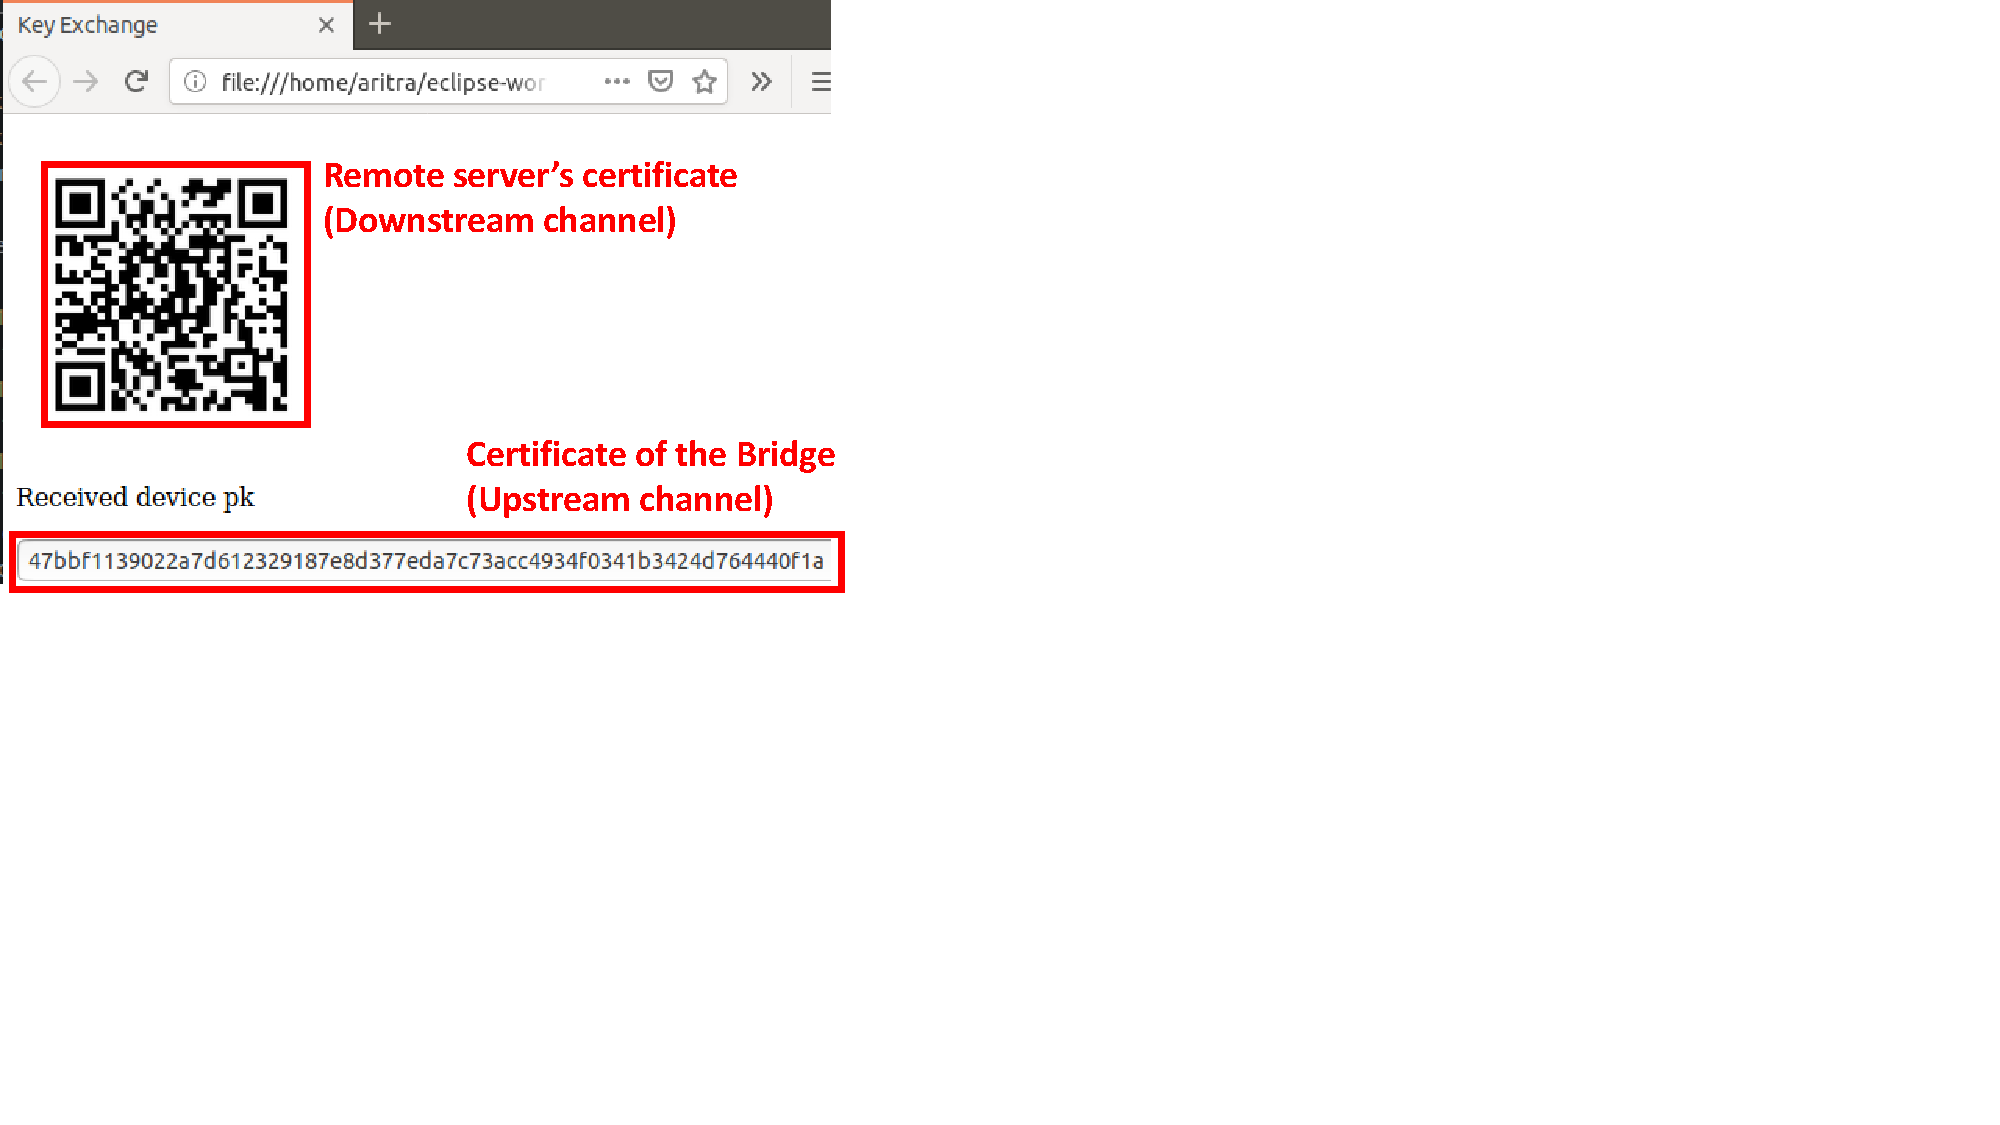
\includegraphics[trim={0 8cm 18cm 0}, clip, width=0.85\linewidth]{keyExchange.pdf}
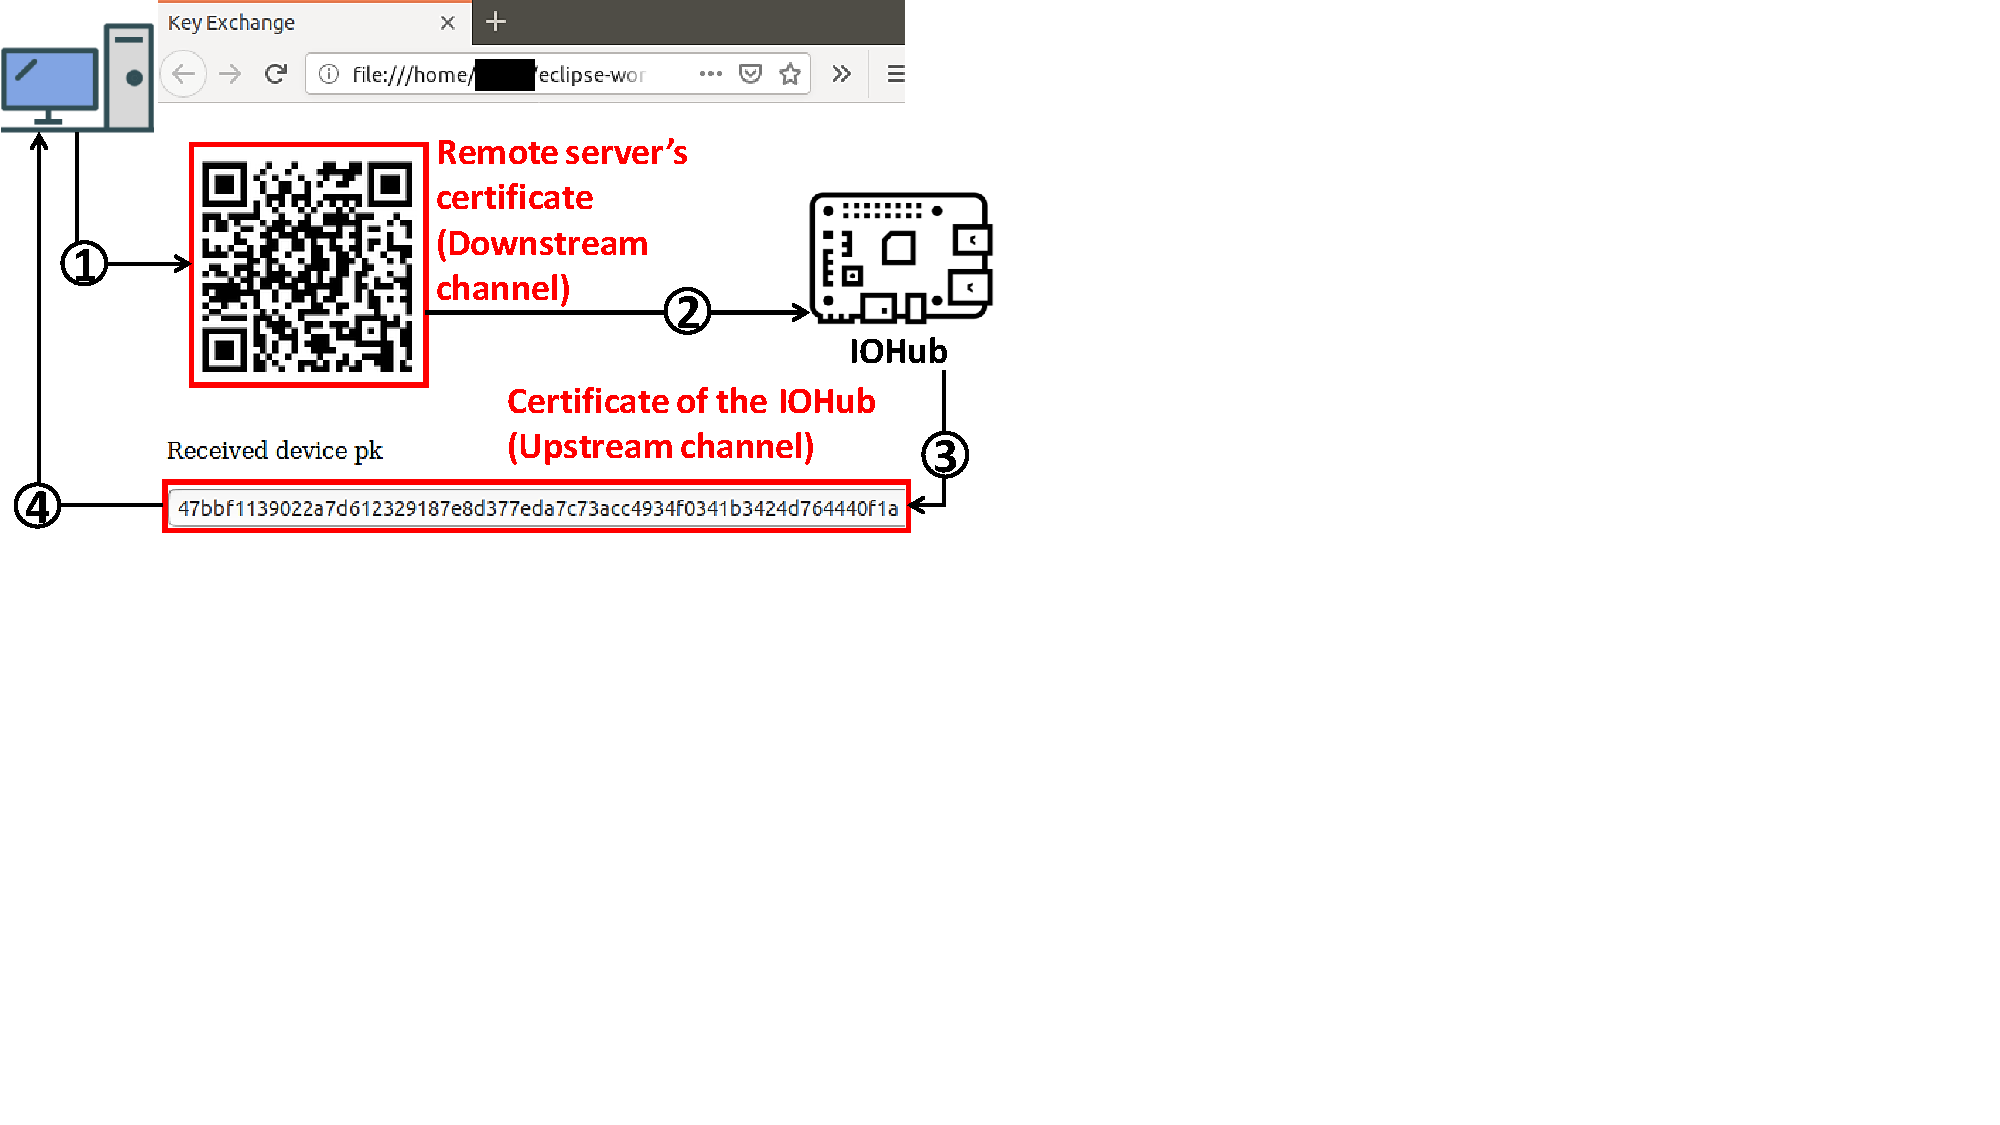
\includegraphics[trim={0 10cm 17cm 0}, clip, width=0.85\linewidth]{keyExchange_1.pdf}
\caption{\textbf{Establishing \tls.} A snapshot of the key exchange web page that is used to communicate the public certificates of the device and the remote server. This page only lasts for a few milliseconds. Hence the page is practically invisible to the user. The QR-code displayed on the web page serves as the downstream channel from the remote server to the \device, whereas the text field is the upstream channel.}
\spacesave
\label{fig:keyExchange}
\centering
\end{figure} 

Note that as described in the system model (see Section~\ref{sec:approach:systemAttackerModel}), the \device lacks any network capability. Hence the \device relies on the untrusted host as the communication channel. Remember that the \device and the remote server already has a bidirectional channel. The downstream channel is the encoded UI specification (see Section~\ref{sec:systemDesign:transformation}) sent by the server and the \name \js provides the upstream channel (see Section~\ref{sec:systemDesign:commit:upload}). 
When the user opens up a webpage that supports \name mechanism, key exchange is the first step that is executed by the \device. Also, the key exchange phase is crucial as the remote server also decide if the user has a \device. We assume that the remote server already has the \device's certificate, or some offline registration takes place. An instance of the key exchange mechanism of \name is illustrated in Figure~\ref{fig:keyExchange}. The flow of the key exchange mechanism is as the following:

\begin{mylist}
  \item[\one] The remote web server serves the web page that shows a QR code that encodes the signed public key of the remote server (server hello in TLS). This page has a $5$ seconds timeout.
  \item[\two] The device captures the frames and looks for a QR code. As soon as the device finds one, the device decodes the QR code and verifies it. If the verification is successful, the device emulates itself as a keyboard device to the host system. The device then encodes its signed public certificate to hexadecimal and send it as a keystroke to the host (client hello in the TLS). For signature, the \device uses the root key of the device manufacturer.
  \item[\three] \name  JavaScript snippet looks for the keystrokes, and as soon as it gets a string of a specific length, it sends the key strokes to the remote server.
  \item[\four] The remote server gets the signed certificate from the \device,. If the verification is successful, the server derives the shared secret.
 
\end{mylist}

After this, both the device and the remote server have each other's public certificates. Using these certificates, both the \device and remote server calculates the shared secret using the authenticated Diffie-Hellman protocol~\footnote{Assume that $(g^x, x)$ and $(g^y, y)$ is the public-private key pair of the remote server and the \device respectively, where $g$ being a generator of a group $G$. The remote server sends a QR code that encodes a CA-signed $g^x$. The \device transmits signed $g^y$ to the remote server. Both the remote server and the \device computes $g^{xy}=(g^x)^y=(g^y)^x$ as the shared secret. Detailed description can be found  in~\cite{blake1998authenticated}.}. In the case the user does not have a \device, the step mentioned above does not take place within the $5$ seconds timeout period. In that case, \name JavaScript snippet concludes that the user does not have a \device. This allows the webpage to fallback to conventional web UIs that do not involve \device for their operation.


\subsection{IO Operations}
\label{sec:confidentiality:io}

\lstset{language=HTML, frame=tb, caption=\small{\textbf{HTML page from the remote server that contains the encrypted UI specification for IO confidentiality.}} , label = snippet:encryptedHTML, firstnumber =1}
\begin{figure}[t]
\small
\begin{lstlisting}[mathescape=true]
<form action="/some_action">
  Text box 1:<br>
  <input type="text" name="text_box_1">
  <br> text box 2:<br>
  <input type="text" name="text_box_2">
  <encrypted_qr><!-encrypted UI specification->
  0x4a5c4... </encrypted_qr>
  <script> [JS outputs QR code that encodes 
  encrypted specification] </script>
</form> 
\end{lstlisting} 
\end{figure}



\begin{figure}[t]
\centering
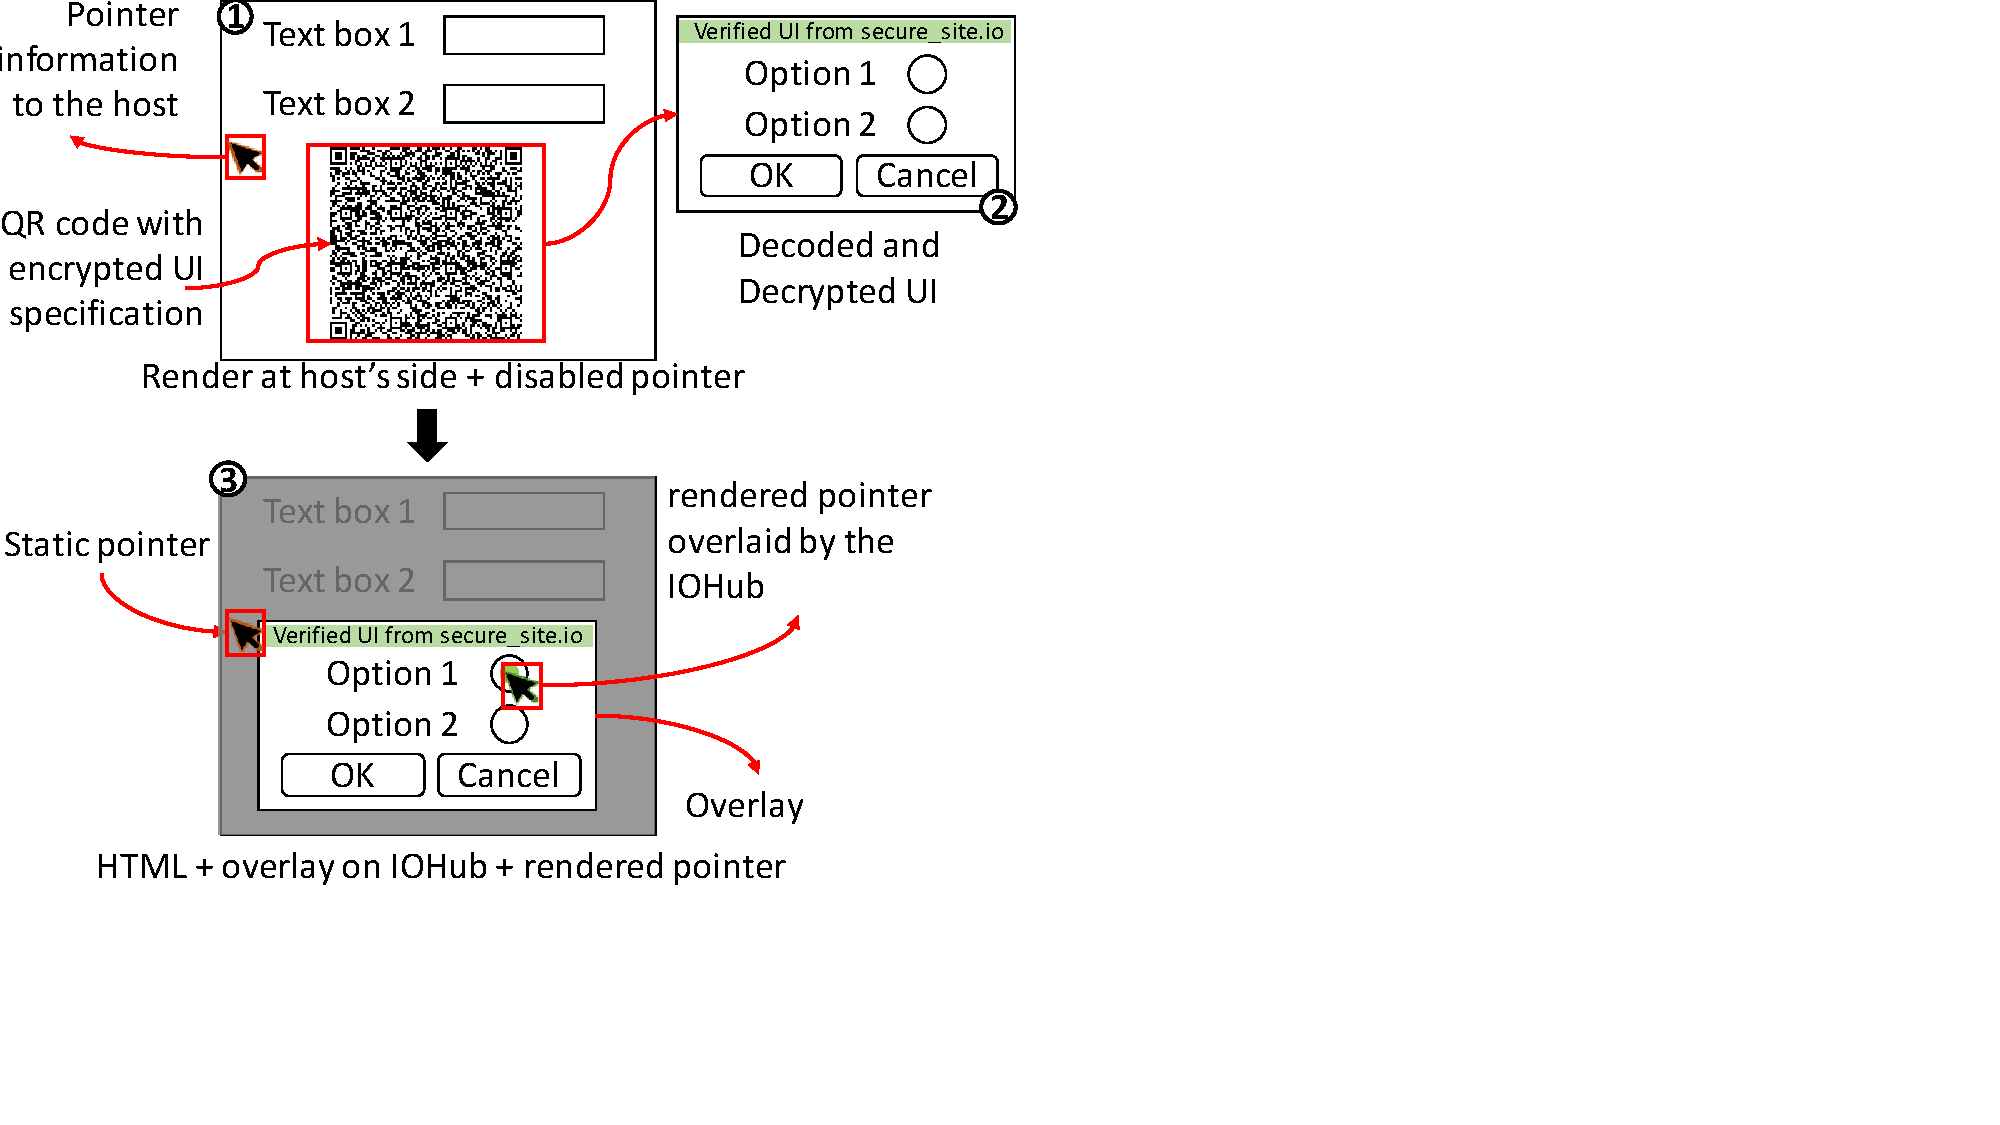
\includegraphics[trim={0 3cm 16.5cm 0}, clip, width=0.88\linewidth]{activityPrivacyRender.pdf}
\caption{\textbf{IO confidentiality.} The figure shows how \name achieves the confidentiality of the UI elements and the mouse pointer in the presence of a compromised host. The upper screenshot shows the host's view of the display while the lower one shows the user's view. The host can only see a QR code where the specification is encrypted by the \tls session key between the \device and the remote server. The user saw the decoded and overlaid UI objects that are retrieved from the QR code sent by the remote server (as described in Section~\ref{sec:systemDesign:transformation}).}
\spacesave
\label{fig:activityPrivacy}
\centering
\end{figure}

After the server and the \device establish the \tls channel, \name is ready to provide IO confidentiality.

\myparagraph{Output confidentiality} Output confidentiality ensures that no information sent from the remote server is visible to the host. To enable output confidentiality, the UI overlay mechanism that is described in Section~\ref{sec:systemDesign:transformation} is modified slightly. Here we \name does not require \name JS to transform all the UI elements to QR code specification. A small server-side module that is very similar to \name JS transforms the UI elements to the UI specification (one such specification is provided in Specification~\ref{snippet:UISpecification}) and encrypt the specification with the \tls session key (Section~\ref{sec:confidentiality:tls}). The \device decodes the QR code from the intercepted HDMI frames, decrypts the specification and overlays the UI on the HDMI frames. One example is provided in the HTML Snippet~\ref{snippet:encryptedHTML} where the \texttt{<encrypted>} tag contains the encrypted UI specification from the server. The \name JS (inside \texttt{<script>} tag) encodes this encrypted UI specification to a QR code.

\myparagraph{Input Confidentiality} When the user enters her mouse pointer into the overlaid UI boundary, the \device stops transmitting any mouse data to the output system, making the host completely oblivious to any mouse movement done by the user. Likewise, when the user selects a UI element, for example, a radio button that is shown in Figure~\ref{fig:activityPrivacy}, the \device encrypts and signs the packets and sends the packet to the remote server making the input commands/values hidden from the attacker-controlled host.  


\section{Security Analysis}
\label{sec:securityAnalysis}

%In this section, we analyze the security of \name by modeling the interaction between the user, host, and the remote server.


\myparagraph{Modelling the user behavior} Correctly understanding the user behavior is critical as \name focuses on securing user interaction with the remote server. In Section~\ref{sec:systemDesign:userAttention}, we explain how to focus user attention using techniques such as lightbox or freezing. Note that these mechanisms are activated automatically for IO integrity by the \device when the user enters the sensitive UI. However, for IO confidentiality, as we discussed in Section~\ref{sec:confidentiality:SAS}, \name requires secure attention sequence (SAS) to be activated by the user. SAS enables the user to i) recognize which part of the screen is overlaid by the \device, and ii) follow the legitimate mouse pointer. We assume that the user behaves reasonably, hence the SAS mechanism is sufficient to isolate the trusted part of the screen (\device overlay) from the untrusted part of the screen. We also agree that system like \name may not achieve absolute security as the user may choose to ignore all visual cues made by the \device and choose to follow the untrusted notifications from the host. Therefore, as long as the user does not get influenced by the information provided in the untrusted part of the screen and modifies her input, the \name remains secure.\red{Assumption is vague, could be interpreted at extremes.}

Next, what follows are the informal security analysis of the integrity and confidential properties of \name. Due to space constraints, we provide formal proofs in Appendix~\ref{appendix:security}.


\subsection{Integrity}
\label{sec:securityAnalysis:integrity}

\myparagraph{Interdependency of input and output integrity}  We model the interactions between the user, the remote server and the attacker-controlled host as a finite state machine (FSM) that is depicted in Figure~\ref{fig:fsm} in Appendix~\ref{appendix:security:protocol}. The nodes in the FSM, namely \user, \server, and \host denote the user, server, and the host, respectively. The state transition happens when a node delivers a packet to another node. $m$ defined the message that is sent by \server to \host. $m$ contains the HTTP response (HTML, \js etc.) from the server. $[m']$ denotes the transformation of $m$, that is the webpage rendered by the host. Note that for an honest host, $[m]$ denotes the ideal transformation of $m$. We provide more details about this interaction in Appendix~\ref{appendix:security:protocol}.
Definition~\ref{def:inputIntegrity} and~\ref{def:outputIntegrity} provides the formal definition of input and output integrity respectively. In Theorem~\ref{theorem:th1}, ~\ref{theorem:th2}. and ~\ref{theorem:th3} we prove that as long as user reports everything that she sees on display to the remote server alongside her input over an authenticated channel, input integrity could be achieved. \name ensures output integrity the \device overlays the sensitive UI on the screen. By doing so, \name also ensures input and integrity simultaneously. 

\myparagraph{Changing IO signals} As only the \device can interact with the overlaid UI, the attacker can not manipulate the IO signals inside the overlaid UI. Moreover, the attacker can not generate and submit input data to the remote server as the server requires all the input data to be signed by the \device.

\myparagraph{Attack on the mouse pointer tracking and overlay} 
The attacker may try to defeat the \name pointer tracking and overlay mechanism described in Section~\ref{sec:systemDesign:analysis} by introducing a malicious pointer that is visually more appealing to the user. Note that the \device overlaid mouse pointer is prominent and hard to miss. One can visualize it as an arms race between the attacker and the \device to grab the attention of the user. But, we can argue that this is a suboptimal strategy for the attacker as both of the pointers will be visible on the screen that can cause suspicion to the user. Also, when the real mouse pointer enters the overlaid area, the untrusted part, including the malicious mouse pointer, will be hidden by the focusing mechanism. Hence, we can conclude that executing clickjacking-like attacks is not possible in \name.

\myparagraph{Early form submission} This attack is not possible as all the input (both mouse and keyboard) are connected to the \device and only the \device can interact with the overlaid UI. This makes it impossible for the attacker to emulate a click on the overlaid part of the screen.  

\myparagraph{Replay attack} All the sensitive UI elements from the remote server contain freshness value (nonce) alongside the signature. Hence, the replay attack is not possible.

\myparagraph{Not rendering QR code} The host may deny sending the QR code over the HDMI channel. This is considered as a denial of service, which is acceptable in our threat model as long as the user interacts with a compromised host. 
In any case, the host is not able to alter any user input or access encrypted data when \name with the confidential feature is required.
%However, the \device cannot observe and decode the encoded UI. As the remote server only accepts signed inputs from the \device corresponding to the sensitive UI, the host can not submit arbitrary input values to the remote server.

\myparagraph{Malicious instruction on the screen} The attacker may put malicious instruction/labels on the untrusted part of the screen to influence user inputs. However, when the user enters inside the overlaid UI to send inputs, the focusing mechanism highlights only the secure UI and hides the rest of the screen. 
%The user attention focusing mechanisms enable the user to distinguish the trusted part of the screen from the untrusted part.

\subsection{Confidentiality}

\myparagraph{Redirection} The attacker could redirect the user to a phishing website that renders visually identical UI to that of the legitimate website. Redirection attack cannot break the integrity of the input because a legitimate remote server always requires the signed input from the user. Without a valid signed QR code, the \device never signs the input value. 

The remote server also delivers confidential information only after creating a \tls channel with the user's device. Therefore, if the attacker redirects the user to a malicious page, the legit server does not deliver any information. On the other hand, redirection may compromise only the confidentiality of user inputs if the user does not trigger the SAS mechanism. 
%as the confidentiality of inputs requires the user to manually trigger the SAS to detect any sensitive UI elements that are overlaid by the \device.

\myparagraph{Side-channel leakages} Even though, the \device ensures that no mouse, keyboard events arrive at the untrusted host when the user executes some operation over the overlaid UI, one can not rule out all side-channel leakages. Depending on the application, the amount of time that the user spends or the entry/exit position of the mouse pointer may reveal some information to the attacker. 
\device could allow the remote server to specify additional policies in the specification to prevent side-channel attacks, e.g., a minimum amount of time that the device should not forward any event to the host after the user enters the overlay. We leave as future work defining such policies and implementing them on \name.
%However, for fixed length inputs such as the pin codes or credit card details, do not leak any information about the input.


\myparagraph{Attacks toward \device} In \name trust model, we assume that the \device is trusted. However, in real-world, embedded systems are often vulnerable to attacks as the attacker can use the connection interfaces to reprogram the \device. In our case, the \device has only two interfaces with the host. The HDMI controller on the \device does not support any bidirectional data channel. Hence, the attacker cannot exploit the HDMI interface. The \usb interface on the \device is only unidirectional (\device $\rightarrow$ host) as the \device emulates itself as an HID. Hence the attacker also cannot exploit the \usb interface.  

\section{\name Prototype Implementation}
\label{sec:prototype}


\begin{figure}[t]
\centering
%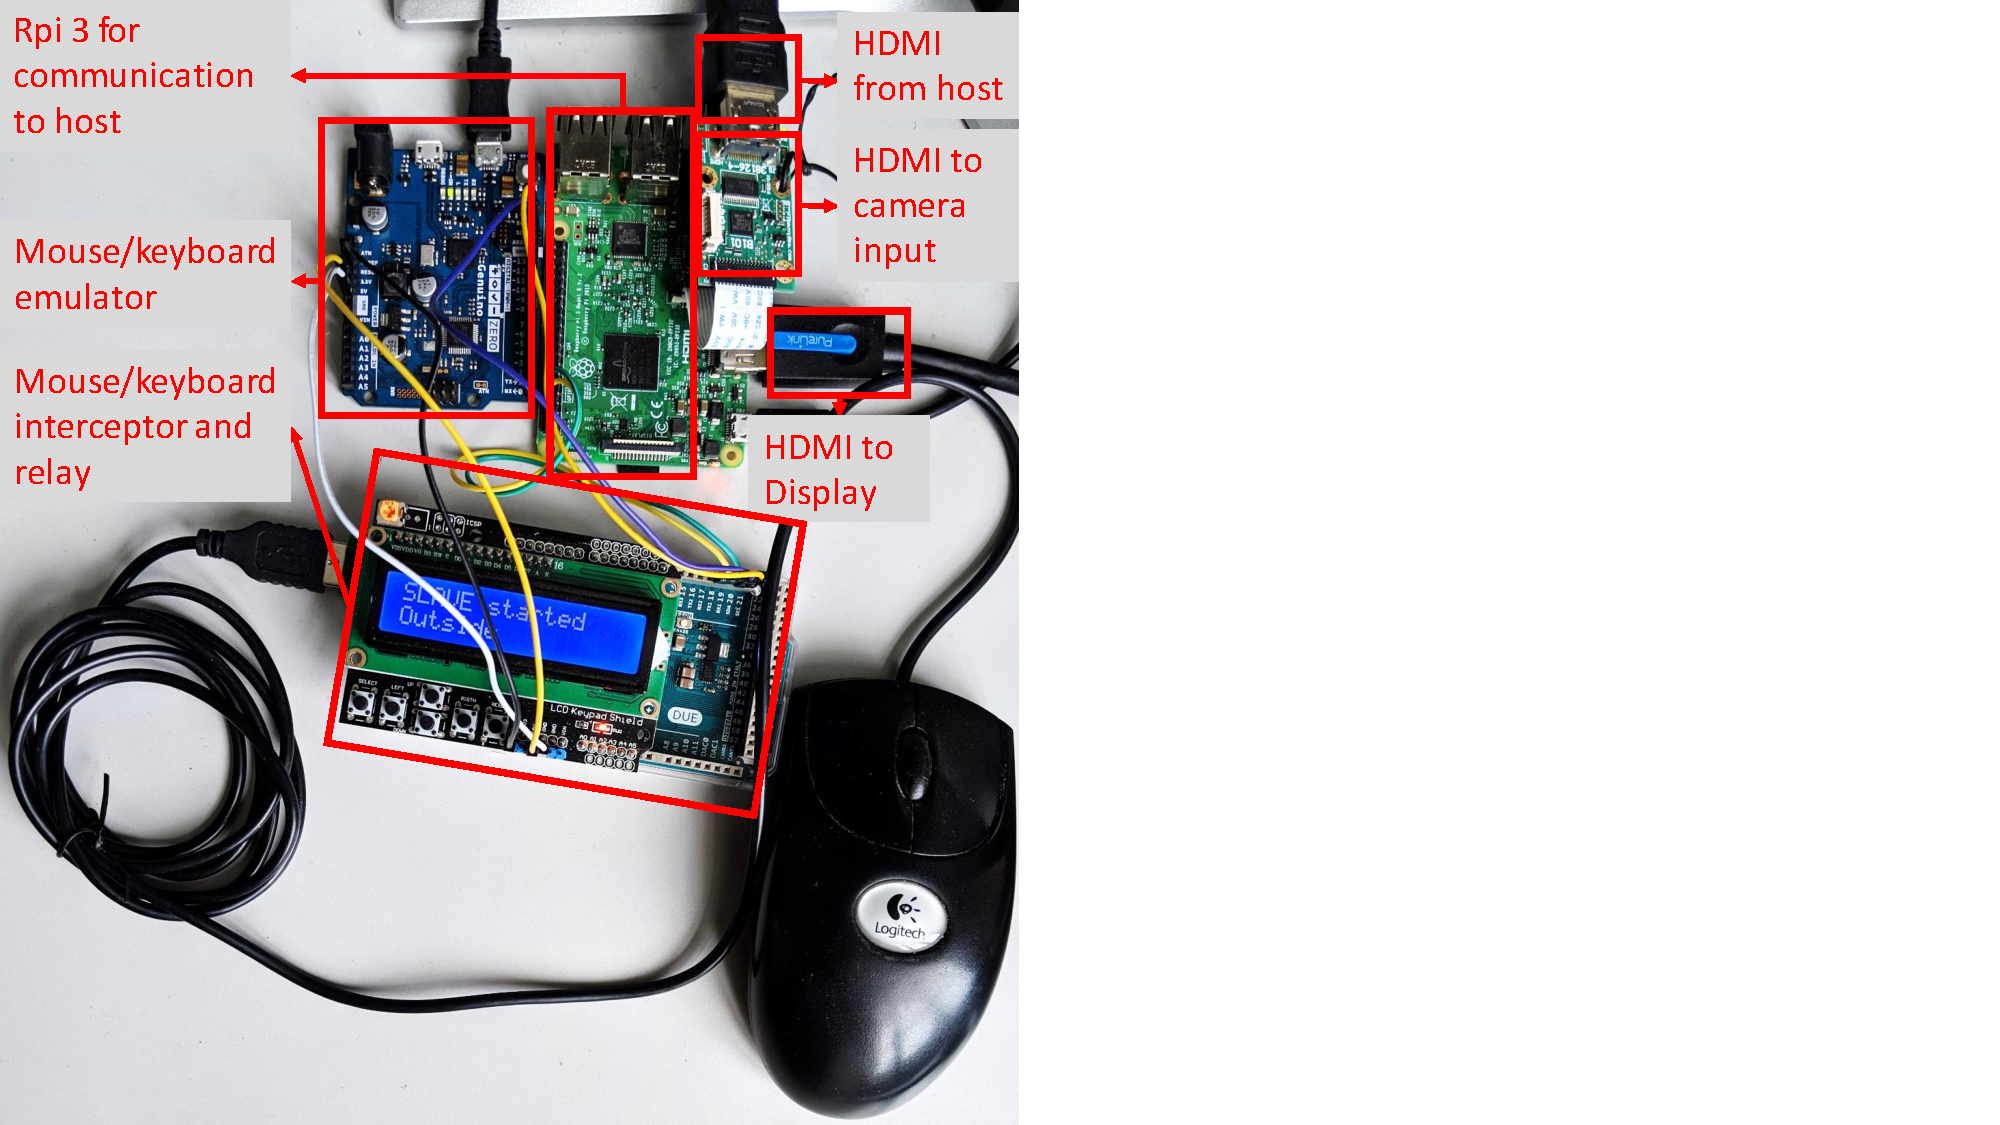
\includegraphics[trim={0 0 15cm 0}, clip, width=\linewidth]{setUp.pdf}
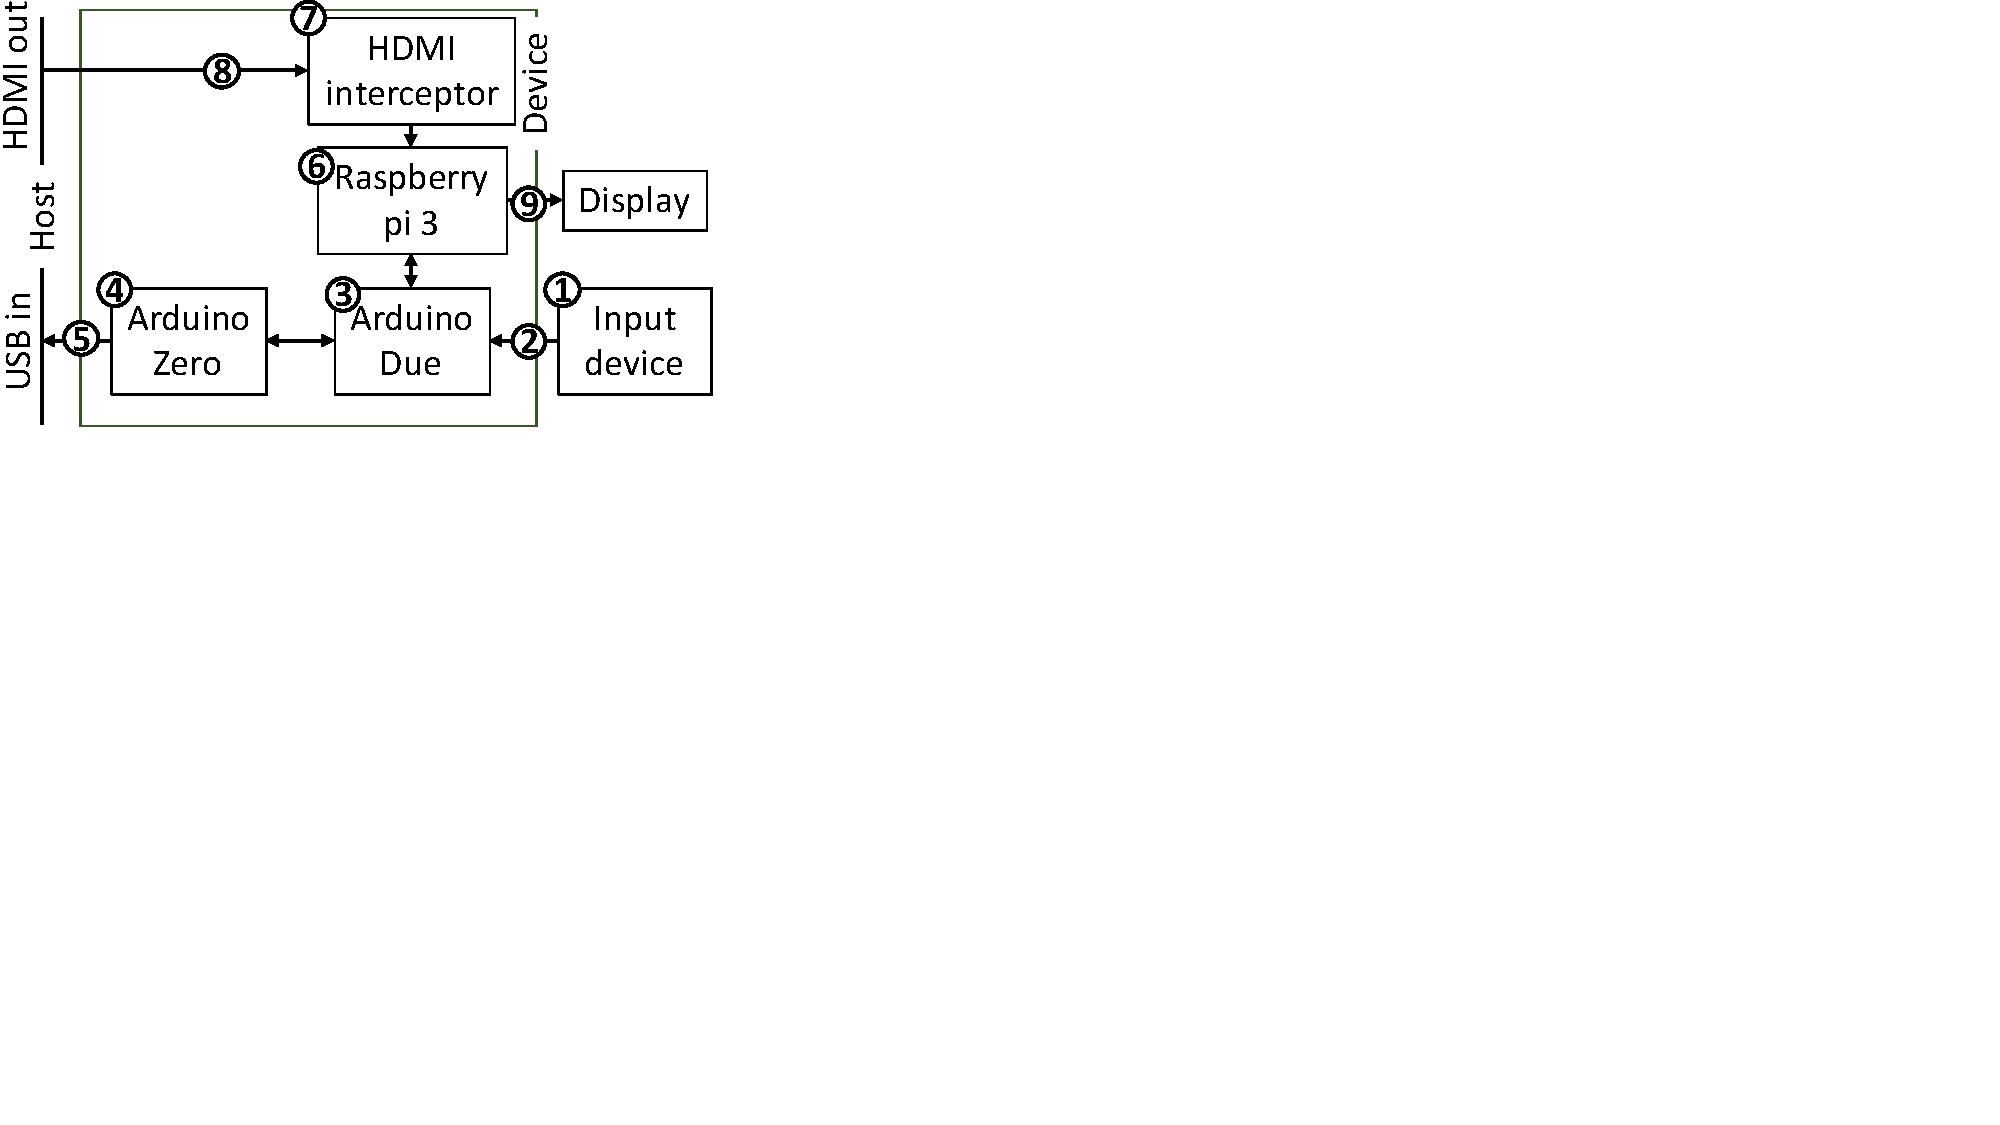
\includegraphics[trim={0 12cm 21.7cm 0}, clip, width=0.7\linewidth]{setUpBlock.pdf}
\caption{\textbf{\name prototype architecture}. }
\label{fig:prototypeArch}
\centering
\end{figure}


\begin{figure}[t]
\centering
%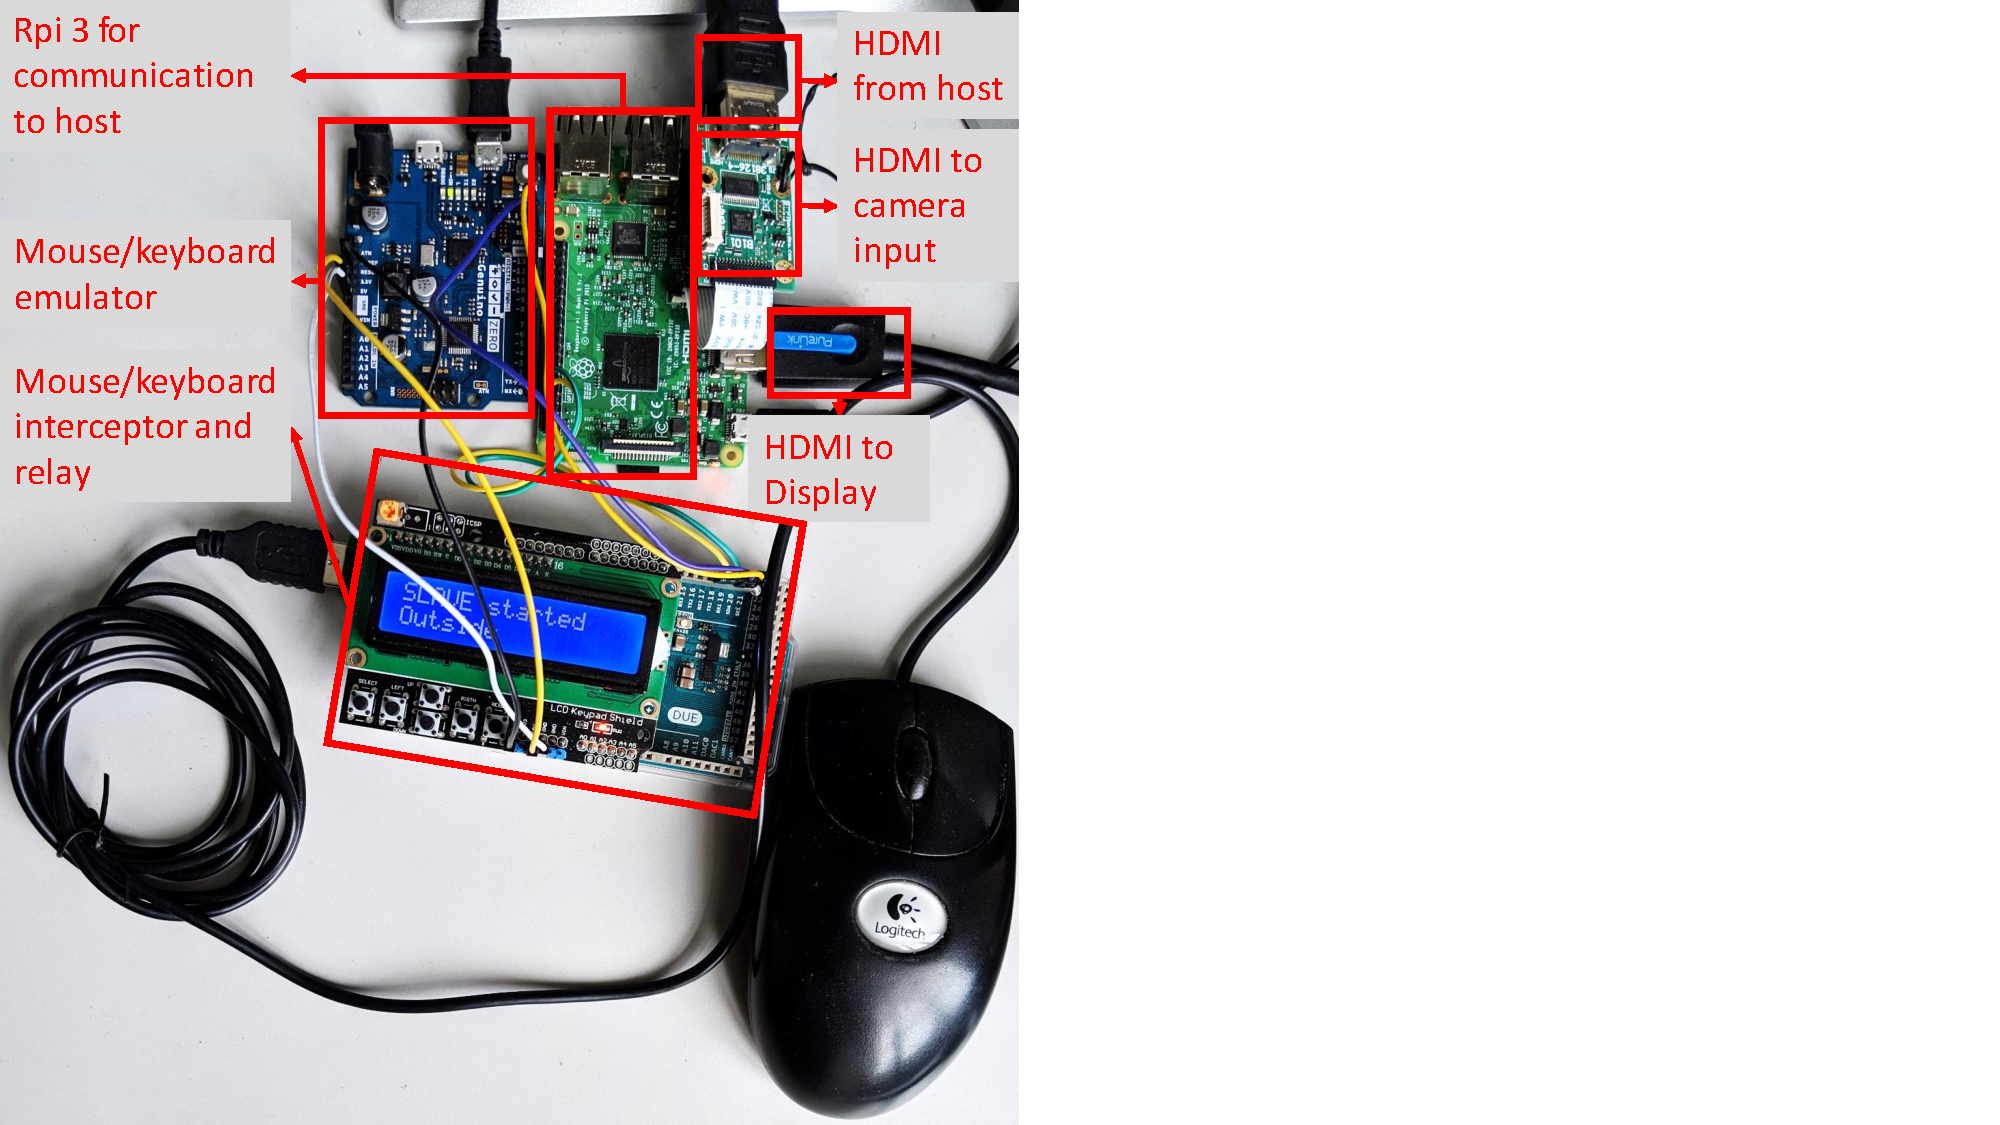
\includegraphics[trim={0 0 15cm 0}, clip, width=\linewidth]{setUp.pdf}
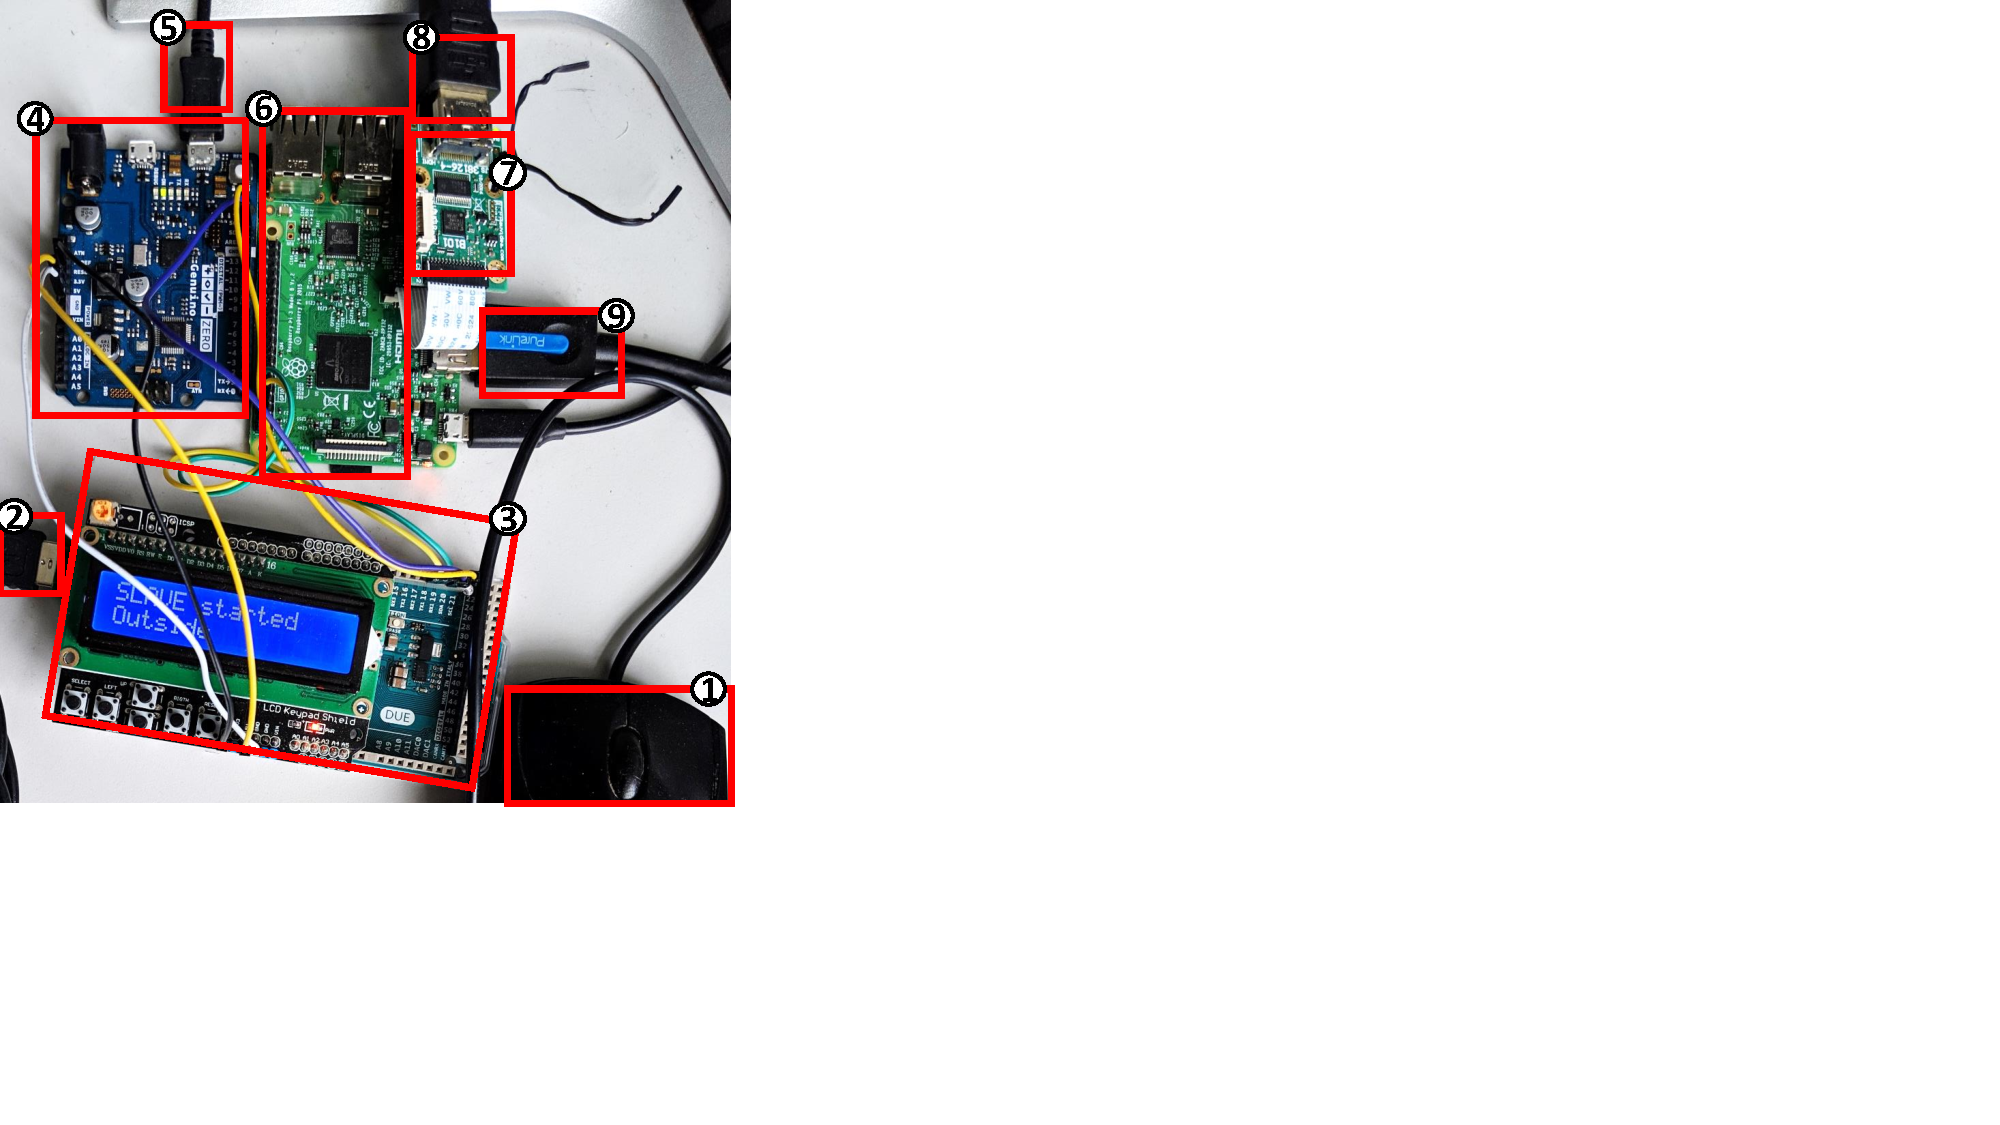
\includegraphics[trim={0 5cm 21.5cm 0}, clip, width=0.75\linewidth]{setUp_1.pdf}
\caption{\textbf{\name prototype}. The figure shows \name prototype that employs Arduino Due and Zero microcontroller board and a Raspberry Pi 3 SBC. The highlighted numbers correspond to the labels in Figure~\ref{fig:prototypeArch}.}
\label{fig:prototype}
\centering
\end{figure}

In this section, we describe our prototype implementation of \name as an auxiliary device. Figure~\ref{fig:prototype} depicts the \name prototype that has the following components

\begin{enumerate}
  \item \textbf{IO interceptor.} The IO interceptor is composed of a  
  \item \textbf{HDMI interceptor.} 
\end{enumerate}
\section{Evaluation}
\label{sec:eval}

\iffalse
\begin{figure}[t]
\centering
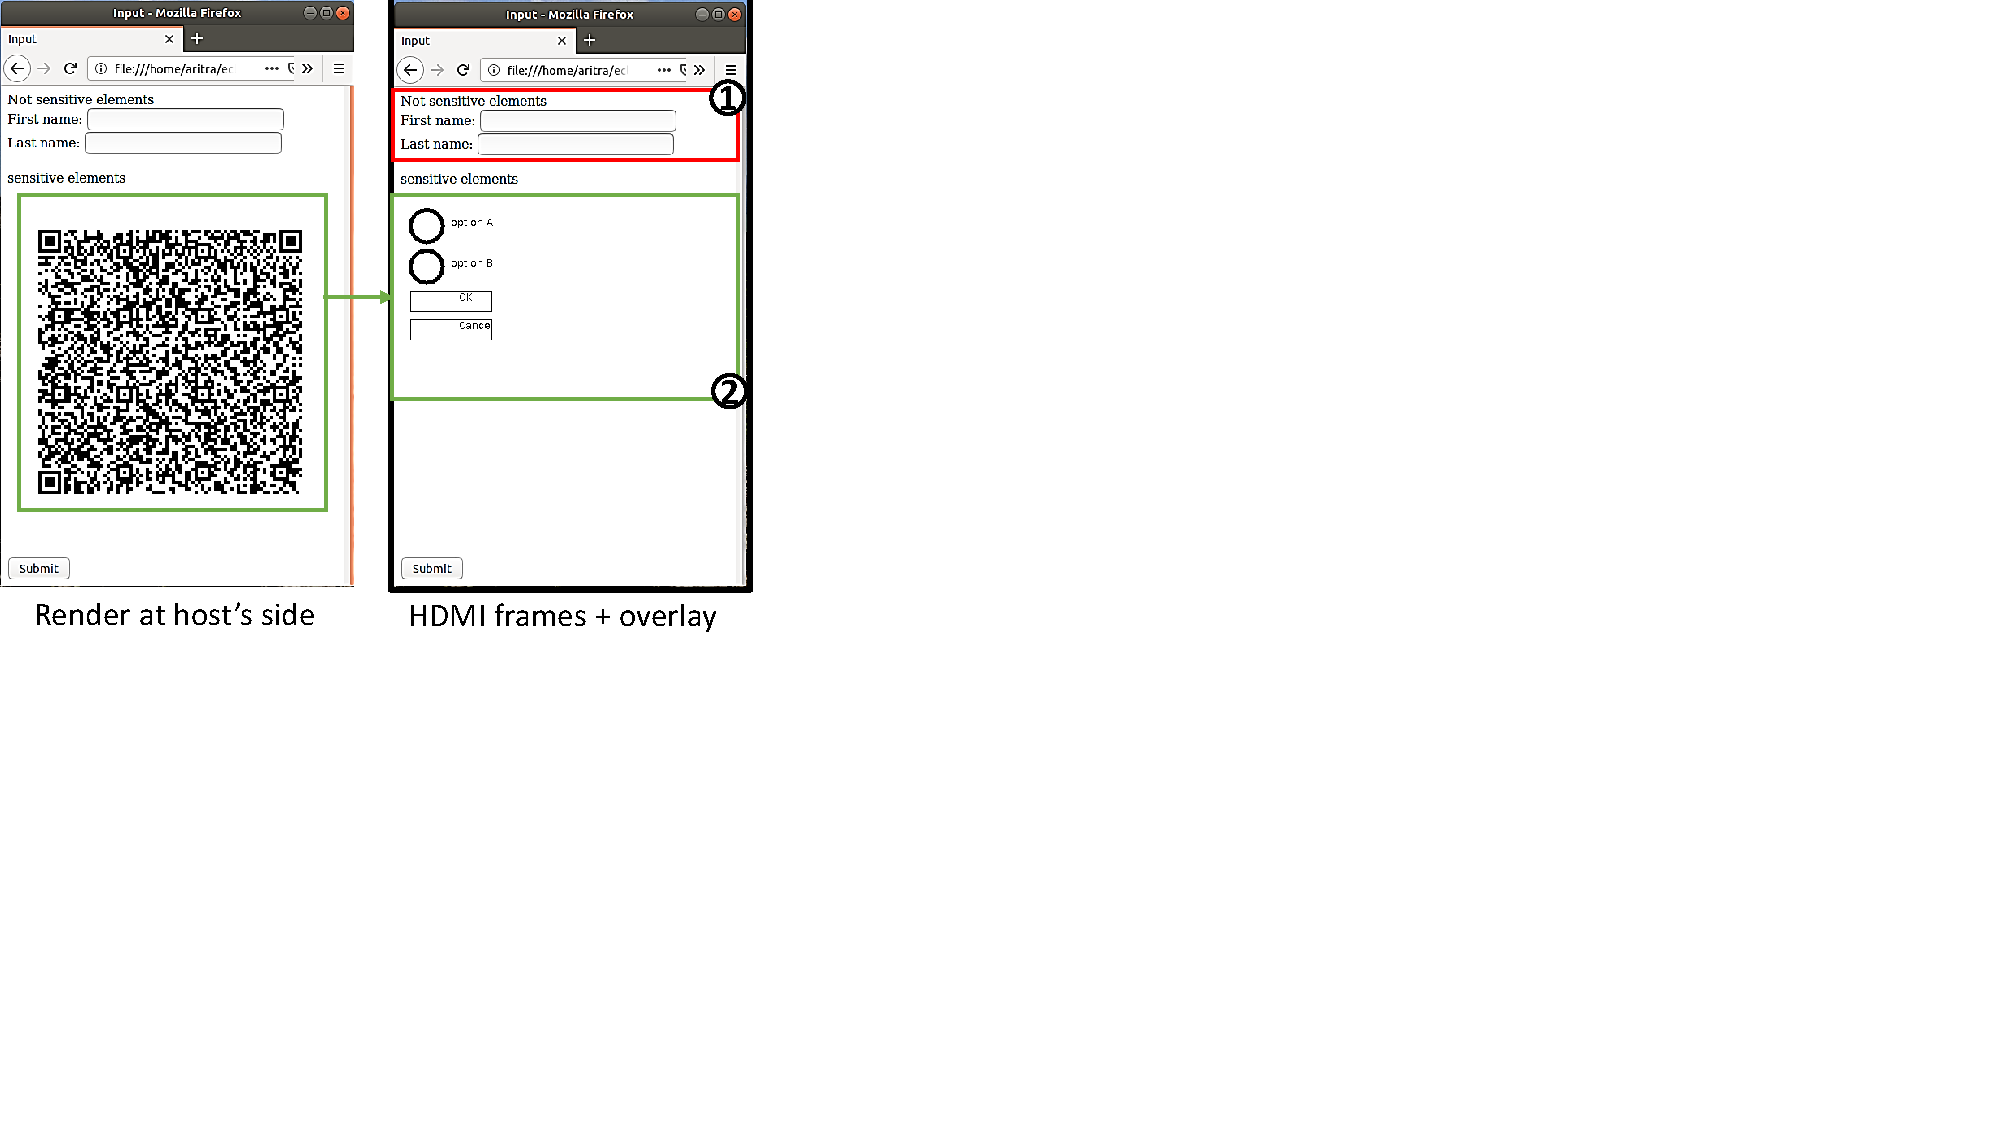
\includegraphics[trim={0 11cm 19cm 0}, clip, width=\linewidth]{overlayScreenShot.pdf}
\caption{\textbf{\name overlay}. }
\label{fig:screenshot_1}
\centering
\end{figure}
\fi


\begin{figure}[t]
\centering
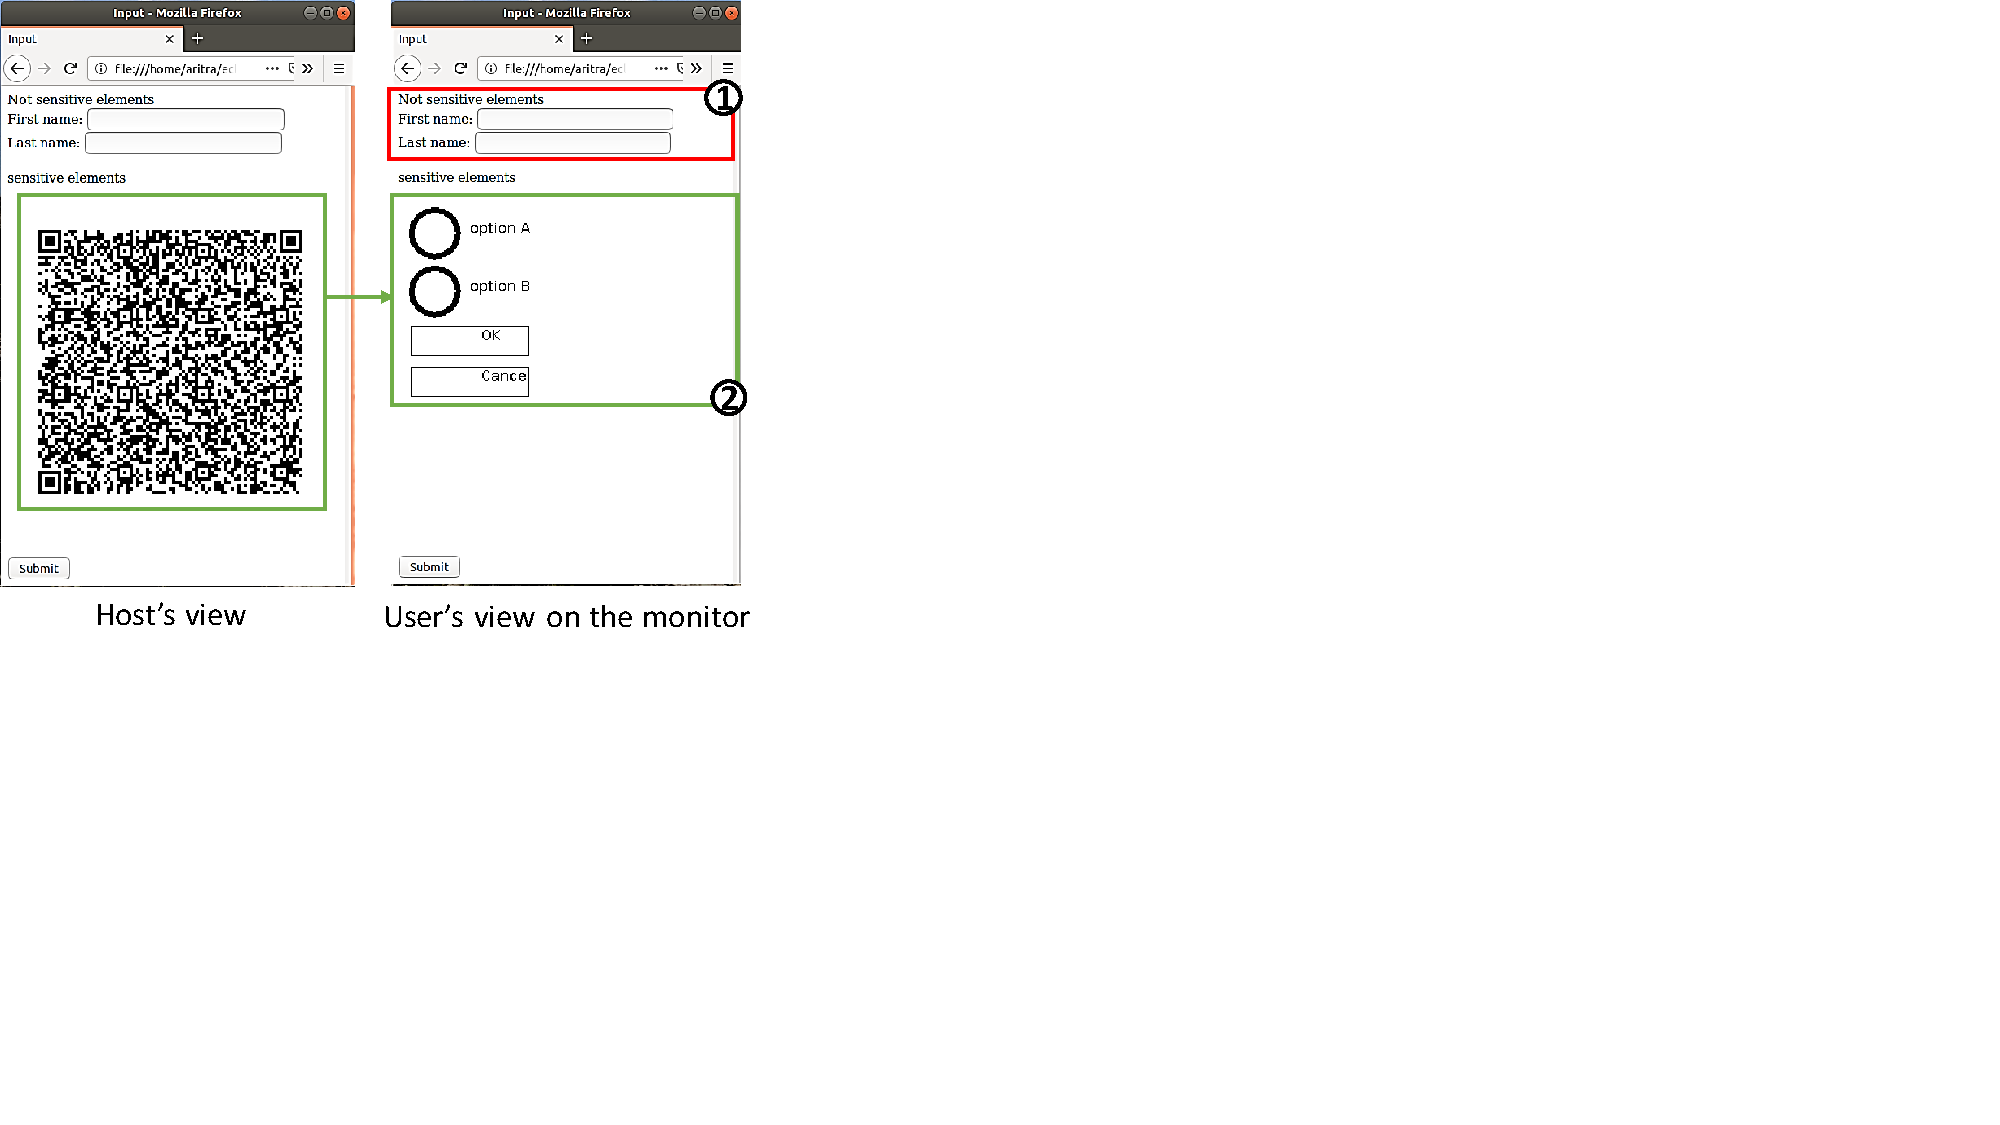
\includegraphics[trim={0 8cm 20cm 0}, clip, width=\linewidth]{overlayScreenShot_1.pdf}
\caption{\textbf{\device generated UI overlay} The figure shows the \name high-level approach. \one shows the non-protected part of the screen where the UI is rendered by the untrusted host. \two shows the \device generated protected UI overlay that is hidden from the host. The protected part of the screen provides integrity and confidentiality of all user IO.}
\spacesave
\label{fig:exampleImpelmentation}
\end{figure}


\begin{table}[t]
%\scriptsize
\centering
\begin{tabular}{l | c}
\textbf{Operation} & \textbf{Average time} \\\hline
Detection QR code & 23 ms\\
Decoding QR code + Overlay & 6 ms\\
Mouse latency & 250 $\mu$s\\
Keyboard latency & 170 $\mu$s\\\hline
\end{tabular} 
\caption{Performance numbers}\spacesave
\end{table}

\subsection{Performance}

We evaluate the performance of our prototype by measuring the overheads introduced by \name to the system and whether they influence the user's interaction. Initially, we measure the default latency introduced by \device when the user interacts with applications that do not require protection. The delay to forward keystrokes is: \red{x ms} and frames is \red{x ms}. (This could be summarized in the end if numbers are very low.)

Our prototype of \name does not require the user to install any additional software in her machine in order to facilitate the communication between the remote server and the \device. Instead, the \device communicates with the remote server by using the host as an untrusted transporter. Therefore, we start by measuring the delay of sending data from the device to the host and vice versa:

\myparagraph{\device $\rightarrow$ host} The \device transmits data (encrypted) to the host by simulating keystrokes. In our system \device sends typical \red{x bytes} of data to the host. This takes \red{x ms}.

\myparagraph{Host $\rightarrow$ \device} The host sends data to the device by encoding them into the HDMI frame. The QR-code is generated locally in the browser and displayed on the screen. For a specification of a form with two/four elements QR-code generation takes \red{x ms}. The \device detects the QR-code, decodes it and creates the overlay. This process takes \red{x ms} for the same form considered previously.
 
For the applications that need protection \name introduces the following delays:

\myparagraph{Initial Page Load} First time the user visits a web page that employs \name, the remote server and the \device should exchange a cryptographic key to protect the communication. This step requires only \red{one additional ajax requst to the server} therefore the delay is relatively low. Initially, the browser encodes server's public key into a QR-code that is decoded by the \device, which sends the response to the server by simulating the keystrokes.

\myparagraph{Frame processing} \device processes every frame of the host. This takes \red{x ms} which hopefully is less than the frame rate.

\myparagraph{Keystroke latency} The \device intercepts all user's keystrokes and forwards them to the host or renders in the screen. When rendering on the screen, the latency is \red{x ms}.

\myparagraph{Cursor latency} Similarly to keystrokes, the \device intercepts mouse events also. However, the latency of event forwarding is \red{x ms}.


Key exchange takes around $200$ ms. Frame rate $20-24$ fps. Mouse/keyboard latency \textless$10ms$.
%\section{Use case Scenario}
\label{sec:usecase}

\subsection{Safety-critical Systems}
PLCs, medical devices\ldots

\subsection{Messenger}

\subsection{Online voting}

\subsection{Integration with GPUs}

\begin{figure}[h]
\centering
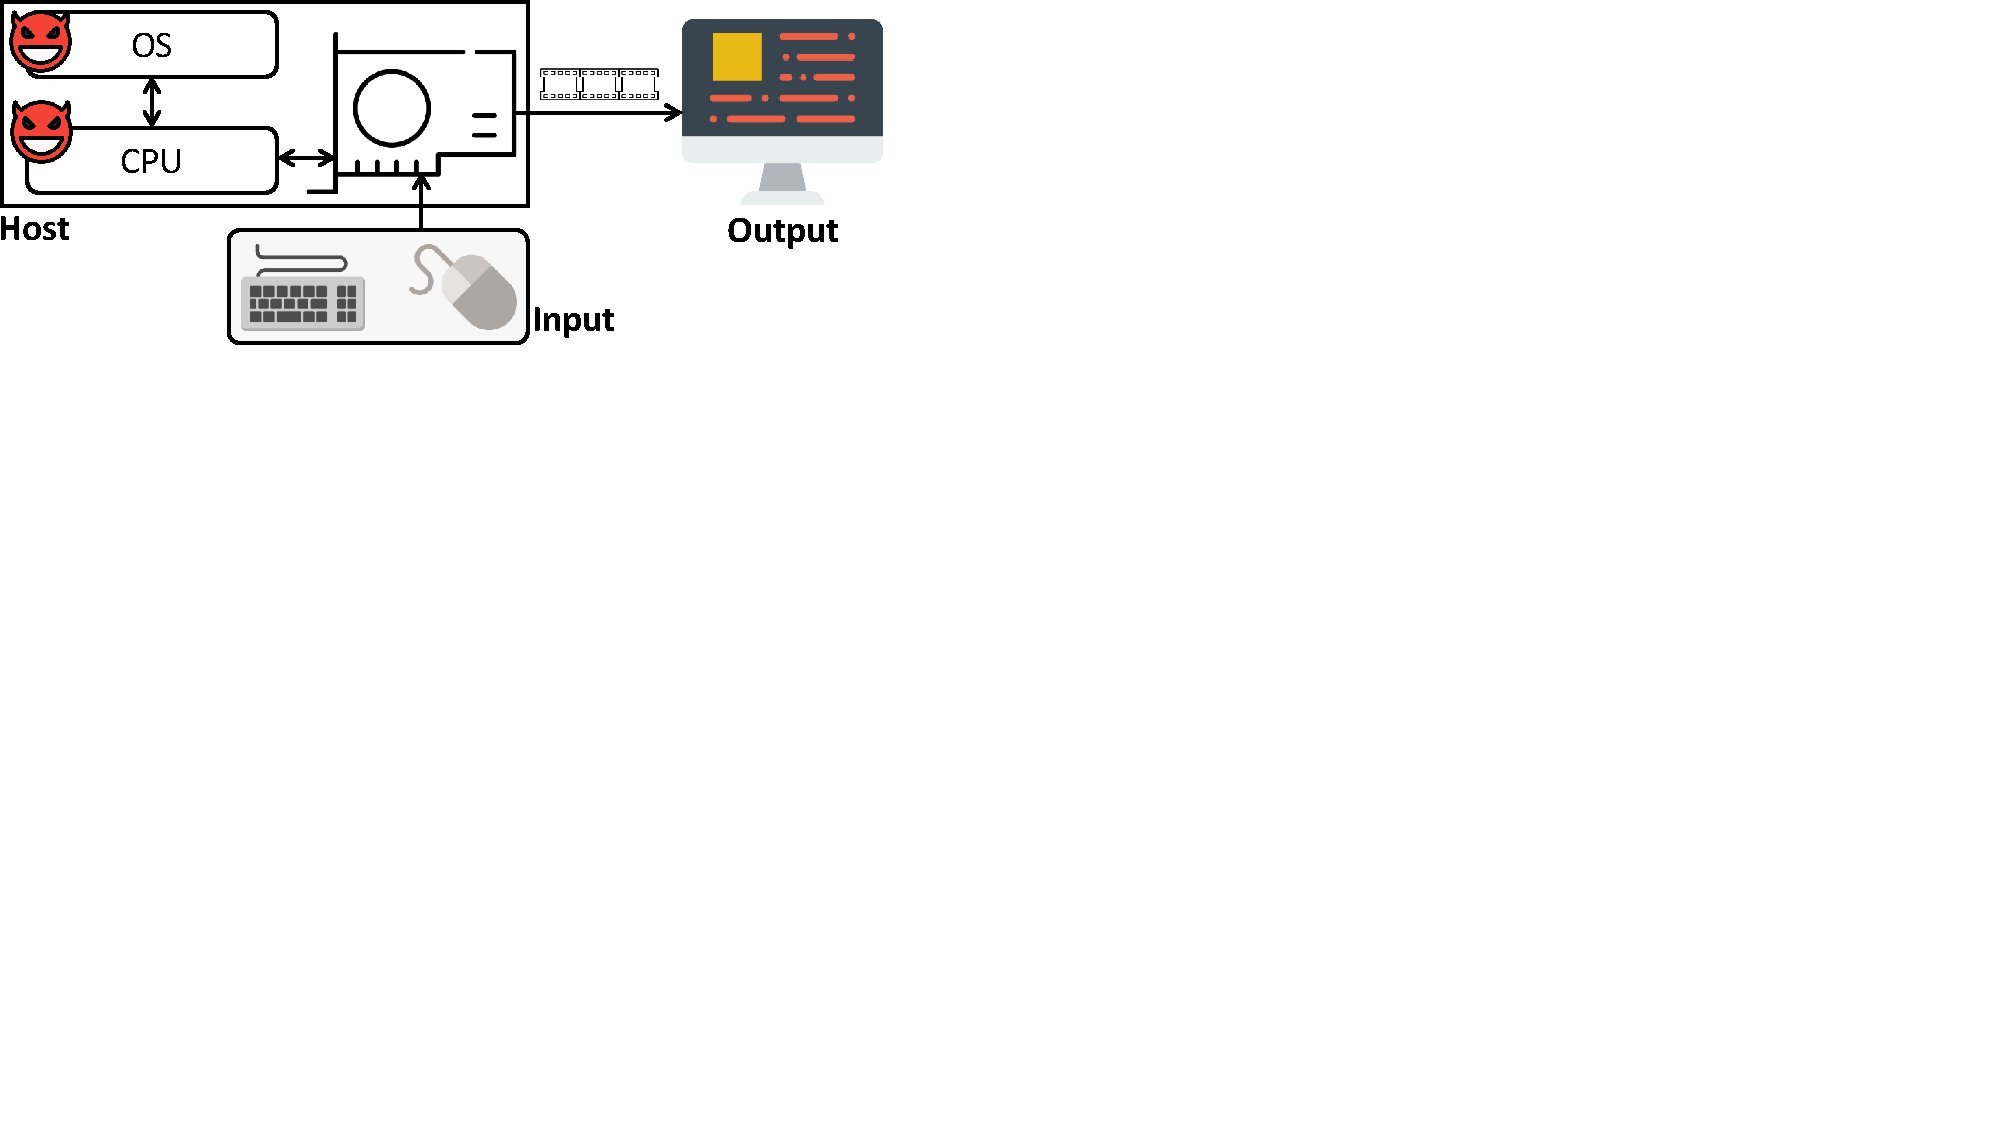
\includegraphics[trim={0 13cm 19cm 0}, clip, width=0.85\linewidth]{graphicsCard.pdf}
\caption{Integrating \name with GPUs}
\label{fig:gpuIntegration}
\centering
\end{figure}
\section{Related Works}
\label{sec:relatedWorks}

Given the attacker's model, there exists several solutions that solve the problem of a trusted path to and from the IO devices in the presence of a compromised host. But all of these solutions targeted for different problem settings and models. Table~\ref{tab:relatedWorks} presents a summarization of such works. We categorize the existing research works into two aspects i) trust assumption, where a lesser number of trust assumption is desirable, and ii) security features that provide integrity and privacy protection for IO. The security features are fine-grained into four sub-features: i) direct input from a keyboard or ii) mouse, ii) mouse pointer movement by the user on top a specific UI element, and iv) output to a display.

Figure~\ref{fig:relatedWorksTree} provides a board classification of the related works and shows where our proposed work stands with respect to them. Detailed description of the relation research is also described in Table~\ref{tab:relatedWorks}.

%\subsubsection{Strawman solution: trusted OS} Trusted OS could be seen as a straightforward solution as traditionally OS handles all the IO drives, computation, and network communications. Assuming a trusted OS significantly reduces the complexity of the solution but the security assumption suffers. Trusted OS introduces a large trusted code base and a multitude of vulnerabilities. 

\subsubsection{Trusted hypervisor/OS-based solutions} Trusted hypervisors and secure micro-kernels are also choices for contrasting Trusted path. Sel4~\cite{klein2009sel4} is a functional hypervisor that is formally verified and has a kernel size of only $8400$ lines of code. In work done by Zhou et al.~\cite{zhou2012building}, the authors proposed a generic trusted path on $x86$ systems in pure hypervisor-based design. Examples of other hypervisor-based works can be found in systems such as Overshadow~\cite{Overshadow}, Virtual ghost~\cite{criswell2014virtual}, Inktag~\cite{hofmann2013inktag}, TrustVisor~\cite{mccune2010trustvisor}, Splitting interfaces~\cite{ta2006splitting}, $SP^3$~\cite{yang2008using}, etc.

In their paper InContext, author Huang et al.~\cite{huang2012clickjacking} presents different clickjacking attacks variants and their solution by using ensuring context (both temporal and visual) and pointer integrity. The pointer integrity is maintained by capturing the screenshot of the UI elements around the pointer and verify with a baseline render of the legitimate UI. The trust model is significantly different from our work as it assumes that the browser and the OS are trusted. Such an attacker model makes the continuous tracking of the pointer unnecessary. Moreover, the clickjacking attack focuses on the cases where the JS served from an untrusted web server tricks the user into clicking on a browser rendered UI (such as the microphone/web camera permission widget that is out of control of the JS). In our case, as we assume the OS/browser to be untrusted, the host can execute arbitrary modification on display. This makes the InConext not directly compatible with the attacker model that \name targets. In summary, InContext looks into some of the properties that \name ensures, namely the context of the user and the pointer integrity but in a completely different problem statement (clickjacking vs. trusted path) and trust assumption.

\subsubsection{Trusted Execution Environments} TEEs are other ways to implement a trusted path between the IO devices and the users. Several TEEs such as Intel SGX, ARM TrustZone, TPM, Intel TXT, etc. can be used to achieve such functionality. Previous research works such as Intel SGX and trusted hypervisor-based SGXIO~\cite{weiser2017sgxio}, Intel SGX based ProximiTEE~\cite{dhar2018proximitee}, TPM and TXT based trusted path~\cite{filyanov2011uni}, and ARM TrustZone based trusted path~\cite{filyanov2011uni,sun2015trustotp} are the example of trusted path construction based on TEEs. All of these solutions require specialized platforms with processors that support such infrastructure. In our proposed solution, we concentrate on the non-specialized hardware platform where compatible TEE technologies may not be available. VButton~\cite{li2018vbutton} uses ARM TrustZone to overlay buttons on the mobile devices that conforms if the user taps on certain buttons. Our solution is fundamentally different from VButtion as i) VButtion is specifically tuned for mobile devices, employing ARM TrustZone where as our solution is much generic and targets specifically PCs, and ii) mouse input is significantly different than touch based input as mouse input involves continuous movement where the touch, or taps are discrete events.

TEE primarily provides execution privacy and code integrity. In most of the cases, IO is still mediated by the OS. To mitigate this, may existing research (SGXIO~\cite{weiser2017sgxio}) requires the IO drives to be implemented inside the TEE or using trusted hypervisor that extends the size of the TCB significantly. Moreover, TEE requires trust assumption on the processors and additional code bases. One such example is Intel SGX where the trust model includes the physical processor package, SGX SDK, quoting enclave, launch enclave and Intel attestation service. Our proposed solution avoids such extensive trust assumptions and assumes that the entire platform is in control of the attacker.

\subsubsection{Browser-based solutions} In their paper InContext, author Huang et al.~\cite{huang2012clickjacking} presents different clickjacking attacks variants and their solution by ensuring context (both temporal and visual) and pointer integrity. The pointer integrity is maintained by capturing the screenshot of the UI elements around the pointer and verify with a baseline render of the legitimate UI. The trust model is significantly different from our work as it assumes that the browser and the OS are trusted. Such an attacker model makes the continuous tracking of the pointer unnecessary. Moreover, the clickjacking attack focuses on the cases where the JS served from an untrusted web server tricks the user into clicking on a browser rendered UI (such as the microphone/web camera permission widget that is out of control of the JS). In our case, as we assume the OS/browser to be untrusted, the host can execute arbitrary modification on display. This makes the InConext not directly compatible with the attacker model that \name targets. In summary, InContext looks into some of the properties that \name ensures, namely the context of the user and the pointer integrity but in a completely different problem statement (clickjacking vs. trusted path) and trust assumption.

\subsubsection{Dedicated hardware-based solution} Previous research works such as IntegriKey~\cite{IntegriKey} uses a low-TCB embedded device to introduce a second factor for input integrity. Similar solutions exits such as transaction confirmation devices~\cite{filyanov2011uni} that uses a small display device to show the input parameters to the users.
Such systems are oblivious to the context of the users and the display device hence attacks where attacker selectively drop characters from the text-field are hard to mitigate.  
Fidelius~\cite{Fidelius} uses raspberry pi's and Intel SGX to create a secure channel between the keyboard and the display device. By doing so, Fidelius provides secure input and display for the character-based device - keyboard. Additionally, Fidelius uses overlay to hide the keyboard input from the compromised host so that the input is only visible from the user. In their work, Brandon et al. ~\cite{brandon2017trusted} demonstrate screen overlay on Android devices using FPGAs.

Note that majority of the previous works achieve some form of trusted path specifically for keyboard-based input. However supporting mouse and touch-based input, complex and generic user interfaces and protected users' action (such as the movement of the mouse pointer, gestures, etc.) in a privacy-sensitive application is not a trivial task. Without proper analysis of every frame that the host system produces, it is not possible to track user intention. In our knowledge, our proposed solution is the first to provide such security properties including the mouse movement privacy. Moreover, we want to achieve this in the absence of any TEE as the trust model of our scenario is significantly different. 

%\section{Attacks}
\label{sec:attacks}

\subsection{Changing mouse position}
\subsection{Change user selected values}
\subsection{Manipulate the position of the UI elements on the screen}
\subsection{Add mouse cursor to confuse users}
\section{Conclusion}
\label{sec:conclusion}

\red{\name provides a remote trusted path in the presence of an attacker-controlled host. The guiding principles behind our solutions are that (i) user input and output integrity cannot be considered separately, (ii) all user input modalities must be protected simultaneously, and (iii) user input integrity protection should not rely on user tasks that are prone to habituation and easily forgotten. By following these principles, we design a novel system that provide strong user input integrity protection in the presence of powerful adversary that controls the entire host platform.}


\bibliographystyle{IEEEtran}


\bibliography{references}

\appendix
\subsection{Summary of Existing Trusted Path Research}
\label{appendix:summaryResearch}


% \begin{table*}[t]
% %\scriptsize
% \centering
% %\bgroup
% %\def\arraystretch{1.2}
% \resizebox{\textwidth}{!}{
%   \begin{tabular}{l | l | c  c  c  c | c  c  c  c | c c} 
%   	
%     \multicolumn{2}{c}{\multirow{4}{*}{Security Requirements} \ldelim\{{4}{-10mm}[]} & \multicolumn{4}{c}{} & \multicolumn{4}{c}{\cellcolor{Gray}\textbf{R1}} & \multicolumn{2}{c}{} \\
%     \multicolumn{2}{c}{} & \multicolumn{4}{c}{} & \multicolumn{3}{c}{\cellcolor{Gray}\textbf{R2}} & \multicolumn{3}{c}{} \\
%     \multicolumn{2}{c}{} & \multicolumn{8}{c}{} & \multicolumn{2}{c}{\cellcolor{Gray}\textbf{R3a/b}} \\
%     \multicolumn{2}{c}{} & \multicolumn{4}{c}{\cellcolor{Gray}\textbf{R4}} & \multicolumn{6}{c}{} \\ \hline
%    \multirow{4}{*}{Category}
%    & \multicolumn{1}{c|}{\multirow{4}{*}{Solutions}} &\multicolumn{4}{c|}{Trust Assumption} & \multicolumn{4}{c| }{IO Security Features} & \multicolumn{2}{c} {Usability}\\  \cline{3-12}
%    & &\multicolumn{2}{c|}{Hardware} & \multicolumn{2}{c|}{Software} & \multicolumn{3}{c|}{Input} & \multicolumn{1}{c|}{Output} & \\  \cline{3-10}
%    %\rowcolor{Gray}
%     & & Requires & \multicolumn{1}{c|}{External} & Isolated & Hypervisor/ & \multirow{2}{*}{Keyboard} & \multirow{2}{*}{Pointer} & \multicolumn{1}{c|}{\multirow{2}{*}{Touch}} & \multirow{2}{*}{Display} & No & \multirow{2}{*}{PnP}\\
%    \cellcolor{white} & & TEE & \multicolumn{1}{c|}{trusted HW} & API/Drivers & OS & & & \multicolumn{1}{c|}{} & & SI &\\
%    \hline
%     &Browser-based~\cite{ye2005trusted}			 &  		&   	& \yes 		& \yes 	&  	 		&   	&   		& \yesNope &   &\yes\\
%     \rowcolor{Gray}
%    	\cellcolor{white} & InContext~\cite{Overshadow} 				 &  		&  	&  	  	& \yes 	&   			& \yes 	&   		&   &    &\yes\\
%     & Overshadow~\cite{Overshadow} 				 &  		&  	&  	  	& \yes 	&   			&   	&   		&   &  &  \\
%     \rowcolor{Gray}
%     \cellcolor{white}&Virtual ghost~\cite{criswell2014virtual} 	 &  		&  	&  		& \yes 	&   			&   	&   		&   &  & \\
%     &TrustVisor~\cite{mccune2010trustvisor} 		 &  		&  	&  		& \yes 	&  	 		&   	&   		&   &  & \\
%     \rowcolor{Gray}
%     \cellcolor{white}&Inktag~\cite{hofmann2013inktag} 			 &  		&  	&  		& \yes 	&  			 &   	&   		&   &   & \\
%     &Splitting interfaces~\cite{ta2006splitting}  &  		&  	&  		& \yes 	& \yes 			&   	&   		& \yes &  & \\
%     \rowcolor{Gray}
%     \cellcolor{white}&$SP^3$~\cite{yang2008using} 				 &  		&  	&  		& \yes 	& \yes 			&   	&   		&   &  & \\
%     &SGX IO~\cite{weiser2017sgxio}  				 & \yes 	&  	& \yes 	& \yes	& \yes 			&   	&   		&   &  & \\
%     \rowcolor{Gray}
%     \cellcolor{white}\parbox[t]{1mm}{\multirow{-11}{*}{\rotatebox[origin=c]{90}{\textbf{Hypervisor/OS-based}}}}  \ldelim\{{-10}{0mm}[] & SchrodinText~\cite{sani2017schrodintext}	 & \yes 	&   &  	& \yes 	&   			&   	&   		& \yes &  &  \\
%     &BASTION-SGX~\cite{BASTION-SGX}			     & \yes 	&   	&  		&  	& \yes 			&   	&   		&   &  &\yes\\
%     \rowcolor{Gray}
%     \cellcolor{white}&Slice~\cite{azab2011sice}				     & \yesNope &   	&  		&  	&   			&   	&   		&   &  & \\
%     &TrustOTP~\cite{sun2015trustotp}			     & \yes 	&   	&  		&  	& \yes		 	&   	&   		& \yesNope &  &\yes\\
%     \rowcolor{Gray}
%     \cellcolor{white}&VeriUI~\cite{liu2014veriui}				     & \yes 	&   & \yes 		&  	& \yesNope 		&   	&   		& \yesNope &  & \\
% 	&AdAttester~\cite{li2015adattester}			 & \yes 	&   & \yes 		&  	&   			&   & \yesNope 	& \yesNope &  & \\
% 	\rowcolor{Gray}
% 	\cellcolor{white}&TruZ-Droid~\cite{ying2018truz}			     & \yes 	&   & \yes 		&  	& \yes 			&   	&   		& \yesNope &  &\yes\\
% 	&TrustUI~\cite{li2014building}			     & \yes 	&   & \yesNope 	&  	&   			&   	& \yesNope 		& \yesNope &  &\yes\\
% 	\rowcolor{Gray}
% 	\cellcolor{white}&VButton~\cite{li2018vbutton}			     & \yes 	&   & \yes 	&  	& \yesNope 			&   	& \yes 		& \yes &  & \\
%     &CARMA~\cite{vasudevan2012carma}			     & \yes 	& \yes 	&  		&  	&   			&   	&   		&   & \yes & \\
%     \rowcolor{Gray}
%     \cellcolor{white}&\textsc{ProximiTee}~\cite{dhar2018proximitee}&\yes 		& \yes  & \yesNope 	&  	& \yes 			&   	&   		&   &\yes &\yes\\
%      \cellcolor{white}\parbox[t]{3mm}{\multirow{-13}{*}{\rotatebox[origin=c]{90}{\textbf{TEE-based}}}}  \ldelim\{{-13}{0mm}[] & Fidelius~\cite{Fidelius}			   	     & \yes 	& \yes  & \yes 		&  	& \yes 			&   	&   		& \yesNope &   &  \\
%     \rowcolor{Gray}
%     \cellcolor{white}&FPGA-based~\cite{brandon2017trusted}		 &  		& \yes  &  		&  	& \yes 			&   	&   		& \yes &   & \\
%     &IntegriKey~\cite{IntegriKey}				 &  		& \yes  & \yesNope 	&  	& \yesNope 		&  	&  		&  & \yes &\yes\\ 
%     \rowcolor{Gray}
%     \cellcolor{white} \cellcolor{white}\parbox[t]{5mm}{\multirow{-6}{*}{\rotatebox[origin=c]{90}{\textbf{External HW}}}}  \ldelim\{{-6}{0mm}[] &Terra~\cite{garfinkel2003terra}			     &  		& \yes  & \yesNope 	&  	&  			&   	&   		&   &  & \\   
%     
% 	\rowcolor{white}
% 	\cellcolor{white}&\textbf{\name}	    			&  		& \yes  &  		&  	& \yes 			& \yes 	& \yes 		& \yes & \yes & \yes\\
%     \hline
%     \multicolumn{12}{c}{\multirow{2}{*}{\yes~requires/supports \hspace{1cm} \yesNope ~partially requires/supports}} \\
%   \end{tabular}
%   }
%   \caption{\textbf{Summary of existing trusted path solutions} by their trust assumptions, security features, and usability. Note that a lower trust assumption, a high number of security features and high usability are desired from a generic trusted path solution. SI stands for security indicator, while PnP stands for plug and play capability. The table also categorizes the trust assumptions, IO security features and usability in-terms of the security goals that we have (refer to section~\ref{sec:problemStatement:goals}).}
%   \label{tab:relatedWorks}
% \end{table*}


In Table~\ref{tab:relatedWorks}, we summarize the existing research work based on their trust assumptions, IO security features, and usability. Note that it is desirable to have a lower trust assumption, higher security features, and higher usability. The trust assumption is further refined into hardware trust assumption that includes TEE and external trusted hardware, and software trust assumption, which includes isolated device drivers/APIs and trusted hypervisor/OS. The IO security features involve input that includes keyboard, pointer and touch input, and output that only includes the display. Lastly, the usability aspect is divided into two, the requirement of security indicator (SI), and if the solution supports plug-and-play (PnP). PnP implies that the solution can be integrated into the existing system without introducing any major changes into them and supports different architectures and OS out of the box.  


\section*{\name Sequence of Events}
\label{appendix:protocol}

\iffalse
\begin{figure}[t]
\centering
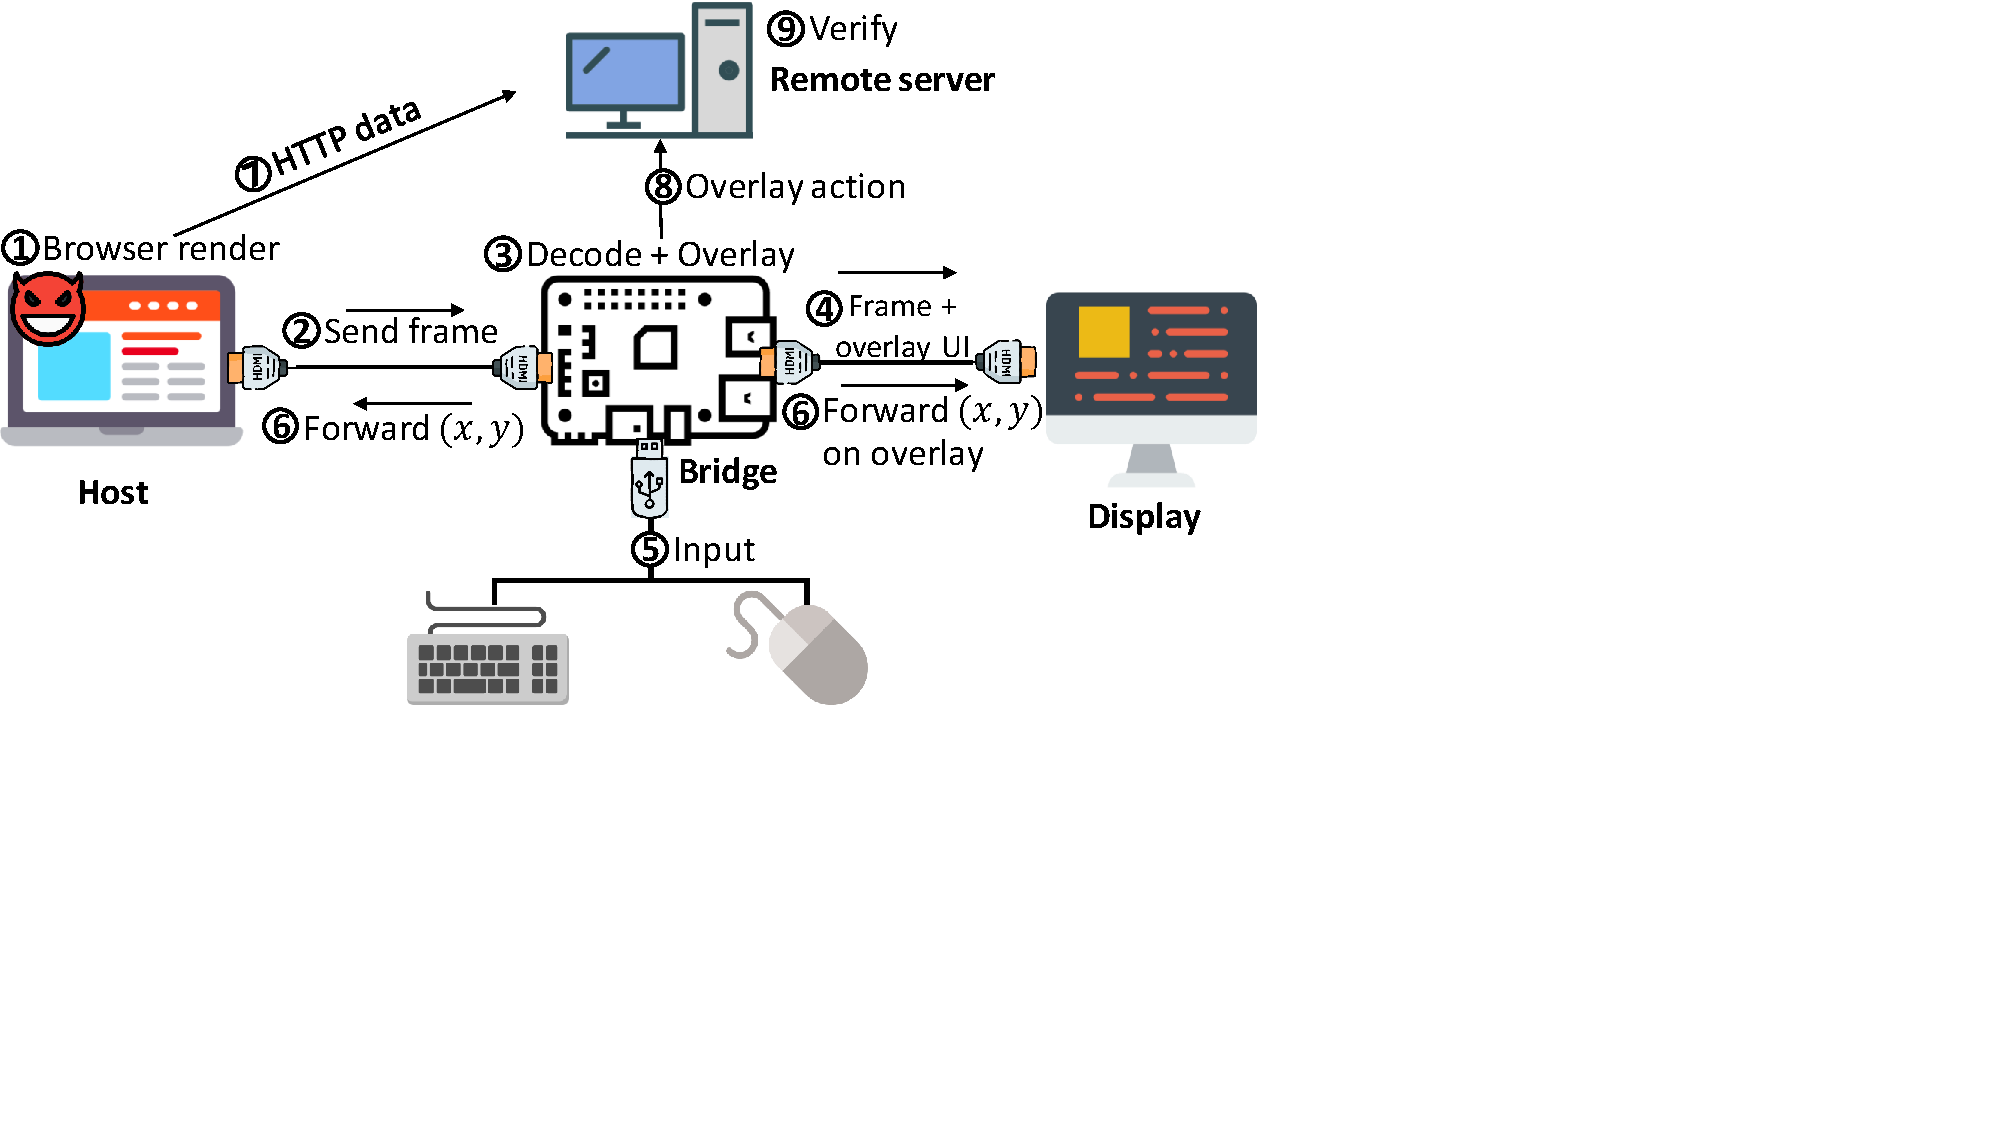
\includegraphics[trim={0 6.5cm 12cm 0}, clip, width=\linewidth]{systemDesign.pdf}
\caption{\textbf{Flow of the \name main protocol.} The figure shows the high-level protocol flow and the main messages that are exchanged between the remote server, host, \device, and the Io devices.}
\spacesave
\label{fig:systemDesign}
\centering
\end{figure}
\fi

Now in this Section, we describe the flow of \name protocol by putting these components together. The outline of \name is illustrated in Figure~\ref{fig:systemDesign}. In the flow, we assume that the user already clicked on a web link or typed the URL in the address bar of the browser. This also allows the \device and the remote server to establish a \tls channel using the method described in Section~\ref{sec:confidentiality:tls}. The rest of the steps are the as the following:


\begin{mylist}
  \item[\one] The browser renders the webpage that comes with \name JS. As described in Section~\ref{sec:systemDesign:transformation}, \name JS transforms the UI elements to a QR code that contains the equivalent UI specification.
  \item[\two] The graphics driver sends the rendered frame to the \device over the HDMI channel.
  \item[\three] The \device intercepts the HDMI signal and decode the QR code to retrieve the UI specification. After the decoding of the QR code, the \device renders the bitmap corresponding to the specification as described in Section~\ref{sec:systemDesign:transformation}.
  \item[\four] The \device send the HDMI frame with the UI overlay to the display device.
  \item[\five] After observing the HDMI frame and the overlaid UI, the user passes her input to the \device via the keyboard/mouse that is connected to the \device over the \usb interface.
  \item[\six] The \device uses raw mouse data and the HDMI frames to interpolate the mouse pointer using the method described in Section~\ref{sec:systemDesign:analysis}. This ensures pointer integrity. \device also overlays a mouse pointer on the HDMI frames.
  \item[\seven] When the user input her data to the host, the \device records her input data (Record phase in Section~\ref{sec:systemDesign:commit:send}).
  \item[\eight] The \name JavaScript snippet also acts as a upstream channel from the \device to the remote server (refer to Section~\ref{sec:systemDesign:commit:upload}). Via this channel, the \device sends the signed user action to the remote server. This signed user action can be seen as the second factor for the integrity of the user input data. (Commit phase in Section~\ref{sec:systemDesign:commit:send})
  \item [\nine] The server verifies the data from the two channels that are submitted by the host and the \device. (Section~\ref{sec:systemDesign:commit:verification})
\end{mylist}


\section*{Formal Proof for IO Integrity}
\label{appendix:security}

In this section we provide a formal proof for the security properties of \name. Namely,  without protecting both input and output integrity, none of them can be achieved. To simplify the proof, we model the interaction between the user, the host and the remote server as a finite state automate (FSA).

\begin{figure}[h]
\begin{center}
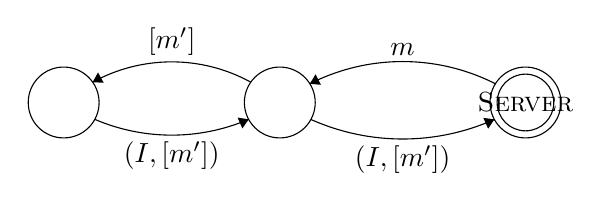
\begin{tikzpicture}[scale=0.15]
\tikzstyle{every node}+=[inner sep=0pt]
\draw [black] (66,-23.1) circle (3);
\draw (66,-23.1) node {\server};
\draw [black] (66,-23.1) circle (2.4);
\draw [black] (45.2,-23.1) circle (3);
\draw (45.2,-23.1) node {\host};
\draw [black] (26.9,-23.1) circle (3);
\draw (26.9,-23.1) node {\user};
\draw [black] (47.743,-21.516) arc (116.95563:63.04437:17.332);
\fill [black] (47.74,-21.52) -- (48.68,-21.6) -- (48.23,-20.71);
\draw (55.6,-19.13) node [above] {$m$};
\draw [black] (29.352,-21.382) arc (118.8302:61.1698:13.89);
\fill [black] (29.35,-21.38) -- (30.29,-21.43) -- (29.81,-20.56);
\draw (36.05,-19.16) node [above] {$[m']$};
\draw [black] (42.565,-24.526) arc (-66.78269:-113.21731:16.527);
\fill [black] (42.57,-24.53) -- (41.63,-24.38) -- (42.03,-25.3);
\draw (36.05,-26.36) node [below] {$(I,[m'])$};
\draw [black] (63.369,-24.535) arc (-65.91058:-114.08942:19.034);
\fill [black] (63.37,-24.53) -- (62.43,-24.4) -- (62.84,-25.32);
\draw (55.6,-26.69) node [below] {$(I,[m'])$};
\end{tikzpicture}
\end{center}
\caption{Finite state machine that depicts the interaction between the user (\user), host (\host) and the server (\server).}
\label{fig:fsm}
\end{figure}

\begin{figure}[h]
\begin{center}
\tikzset{
  every picture/.append style={
    transform shape,
    scale=0.8
  }
 }
\begin{sequencediagram}
\newinst{u}{\user}
\newinst[3]{h}{\host}
\newinst[3]{s}{\server}
\mess{s}{$m$}{h}
\mess{h}{$[m']_1$}{u}
\mess{u}{$I_1,[m']_1$}{h}
%\mess{h}{$[m']_2$}{u}
%\mess{u}{$I_2,[m']_2$}{h}
\mess{h}{...}{u}
\mess{u}{...}{h}
\mess{h}{$[m']_n$}{u}
\mess{u}{$I_n,[m']_n$}{h}
\mess{h}{$I_1,I_2,...,I_n$}{s}
\mess{h}{$[m']_1,[m']_2,...,[m']_n$}{s}
\end{sequencediagram}
\end{center}
\caption{Protocol transcript between the \server, \user and \host that shows one trace from the FSM depicted in Figure~\ref{fig:fsm}.}
\label{fig:protocol}
\end{figure}

\subsection{Interaction Protocol} 
\label{appendix:security:protocol}


The interaction between the server (\server), user (\user) and host (\host) is depicted in the finite state machine in Figure~\ref{fig:fsm}. \server sends a message $m$ to \host. One can assume $m$ to be the HTML, JS send from \server. We denote $[m]$ to be the render of $m$ by the \host. As \host is malicious, it can transform $m$ to $m'$. Note that the transformation is public knowledge and is deterministic. If $m\neq m'$ then given $[m]$ and $[m']$, \server can determine that $[m]\neq [m']$. We denote the user input to be $I$ which corresponds to a specific $[m]$. 
%Note that the communication channel between \server to \user is neither authenticated, neither confidential. But the communication channel from \user and \server is authenticated. 
In this model, we simplify the user input by assuming that the \user only provides an input $I$ only after observing a message transformation $[m]$. The user provides both her input $I$ and transformation $[m']$ observed by her to \host. The interaction loop between \host and \user can continue until \user finishes her input. After every input \host hands over new message transformation to \user (either result of the input or new message from \server or both). Once the user provides all her inputs, \host send the pairs $(I, [m'])$ to \server.

We also define two functions:
\begin{align*}
\texttt{Input()}&:[m]\rightarrow I \\
\texttt{Transform()}&:m,I\rightarrow [m'],\ \exists i\in I:i=\phi
\end{align*}
Both of them are \emph{bijective}.

One trace of the protocol transcript is depicted in Figure~\ref{fig:protocol}. As described in the FSM, \server receives traces of message transformation ($[m']_1,[m']_2,\ldots,[m']_n$) and corresponding inputs ($I_1,I_2,\ldots,I_n$). From these traces \server could determine of all the $[m']_i$ are in proper form by verifying if $[m]_i=[m']_i$.

\begin{definition}{\textbf{Input integrity}}
\label{def:inputIntegrity}
Assume that \server handed a message $m$ to \host where the proper message transformation is $[m]$. The host changes the message transformation to $[m']$ where $[m']\neq [m]$. We also define correct \user input to be $I$ when \host sends a correct message transformation $[m]$ to \user. We define input integrity as the property where the \server does not accept input $I'$ where $I'\neq I$from \user if the \host changes the message transformation.
\end{definition}

\begin{definition}{\textbf{Output integrity}}
\label{def:outputIntegrity}
Assume that \server handed a message $m$ to \host where the proper message transformation is $[m]$. Output integrity defines that in all circumstances, \user receives the correct message transformation $[m]$ from \host.
\end{definition}

\myparagraph{Verification process} \server checks $\forall i=1\ldots n$ $$[m']_i = \texttt{Transform}(m_{i-1}, I_{i-1})$$ where $I_0=\phi$.

\begin{theorem}
\label{theorem:th1}
If \user does not send all the transformations till $[m']_i$ corresponding to the input $I_i$, input integrity can not be achieved. 
\end{theorem}

\begin{IEEEproof}
If \user does not attach all the transformation till $[m']_i$, i.e., $[m']_1, [m']_2, \ldots, [m']_{i-1}, [m']_i$  corresponding to inputs $I_1, I_2,\ldots, I_{i-1}, I_i$, then the server can not verify all the transformations corresponding to the input. \host could modify a specific $[m]_x$ to influence \user input.
\end{IEEEproof}

\begin{theorem}
\label{theorem:th2}
If the channel from \user and \server is not authenticated, input integrity is not achievable. But the channel from \server to \user does not require to be secure as long a \user provides the message transformation $[m']_i$ corresponding to every input $I_i$.
\end{theorem}

\begin{IEEEproof}
The proof is trivial. If the channel from \user to \server is not authenticated, any input provided by \user can be manipulated by \host without a trace. Hence input integrity is not achievable. As long as \user sends message transformation along with the input, a manipulated message transformation bt \host would be detectable by \server (see Theorem~\ref{theorem:th1}).
\end{IEEEproof}

\begin{theorem}
\label{theorem:th3}
Ensuring output integrity also ensures input integrity provided there is an authenticated channel from \user to \server.
\end{theorem}

\begin{IEEEproof}
This proof is also trivial. As we describe in the Definition~\ref{def:inputIntegrity} and~\ref{def:outputIntegrity}, if all the message transform from \host $[m']=[m]$, and \host always executes \texttt{transform()} properly, the input integrity is preserved. As \name ensures output integrity and all the input from the user is signed by the \device, \name preserves input integrity. 
\end{IEEEproof}




\end{document}


%%Abstract submission

% Security and safety-critical remote applications such as e-voting, online banking, industrial control systems and medical devices rely upon user interaction that is typically performed through web applications. Trusted path to such remote systems is critical in the presence of an attacker that controls the computer that the user operates. Such an attacker can observe and modify any IO data without being detected by the user or the server. We investigate the security of previous research proposals and observe several drawbacks that make them vulnerable to attacks. Based on these observations we identify novel requirements for secure IO operation in the presence of a compromised host.
%   
% As a solution, we propose ProtectIOn, a system that ensures IO integrity using a trusted low-TCB device that sits between the attacker-controlled host and the IO devices. ProtectIOn intercepts the display signal and user inputs from the keyboard and mouse, and overlays secure UI on top of the HDMI frames generated by the untrusted host. The guiding design principles of ProtectIOn are that (i) integrity of user input and output cannot be considered separately, (ii) all user input modalities need to be protected simultaneously, and (iii) integrity protection should not rely on error prone user tasks like checking the presence of security indicators. By following these guidelines, ProtectIOn achieves strong protection for IO integrity. We also propose an extension of ProtectIOn for IO confidentiality and implement a plug-and-play prototype and evaluate its performance. 